%-----------preamble-------{{{
\documentclass[a4paper,12pt]{book}
\usepackage{tocloft}
\renewcommand{\cftsecafterpnum}{\quad\rule{1cm}{0.4pt}\quad\rule{2cm}{0.4pt}}
\usepackage{tabularx}
\usepackage[a4paper, left=1in,right=1in,top=2cm,bottom=1.5cm]{geometry}
\usepackage{fancyhdr}
\usepackage{csvsimple}
\pagestyle{plain}
\renewcommand{\chaptername}{Experiment}
\usepackage[utf8]{inputenc}
\usepackage{float}
\restylefloat{table}
\usepackage{pdfrender}
\usepackage{amsmath}
\usepackage{xcolor}
\usepackage{ae}
\usepackage{multirow}
\usepackage{aecompl}
\usepackage{helvet}
\usepackage{afterpage}
\usepackage{graphicx}
\usepackage{caption}
\usepackage{array}
\usepackage{subcaption}
\parindent=10pt
\parskip=5pt
\makeatletter
\newcommand\@addfig{\relax}
\newcommand\addfig[1]{\global\long\def\@addfig{#1}}
\newcommand\@putfig{\@addfig\addfig{\relax}}
\newcommand\blankpage{%
	\null
	\vfill
	\@putfig%
	\vfill
	\thispagestyle{empty}% BEWARE, if you want the header and footer, you should put the correct style here
	\clearpage%
	\addtocounter{page}{-1}% BEWARE, if you want the left pages to be numbered, don't put this line, this is intended to have picture page with the same number as the facing text page
	\afterpage{\blankpage}}
	\makeatother

    \makeatletter
    \renewcommand\part{%
       \if@openright
         \cleardoublepage
       \else
         \clearpage
       \fi
       \thispagestyle{empty}%
       \if@twocolumn
         \onecolumn
         \@tempswatrue
       \else
         \@tempswafalse
       \fi
       \null\vfil
       \secdef\@part\@spart}
    \makeatother

	\begin{document}
	\pagenumbering{roman}
	\tableofcontents
	%\pdfrender{StrokeColor=black,TextRenderingMode=2,LineWidth=0.1pt}
	\afterpage{\blankpage}
%-----------------------}}}
	%-------Hematology----{{{
	
	\part*{Hematology}
	%-------CompoundMicroscope---{{{
	\pagenumbering{arabic}
	\chapter*{\centering Compound Microscope}
\addcontentsline{toc}{chapter}{Compound Microscope}

	\begin{tabular}{p{5in} p{1in}}
		\textbf{Exp No:}  & \textbf{Date:}\\
	\end{tabular}
	\section*{Introduction}
	\par
	A microscope is an optical instrument which magnifies the image of an object.
	There are various types of microscope which use different types of lens and different principles of optics.
	Compound microscope is one of the most frequently used equipment in a medical laboratory.\newline

	\addfig{%
		\begin{figure}[h]
			\centering
			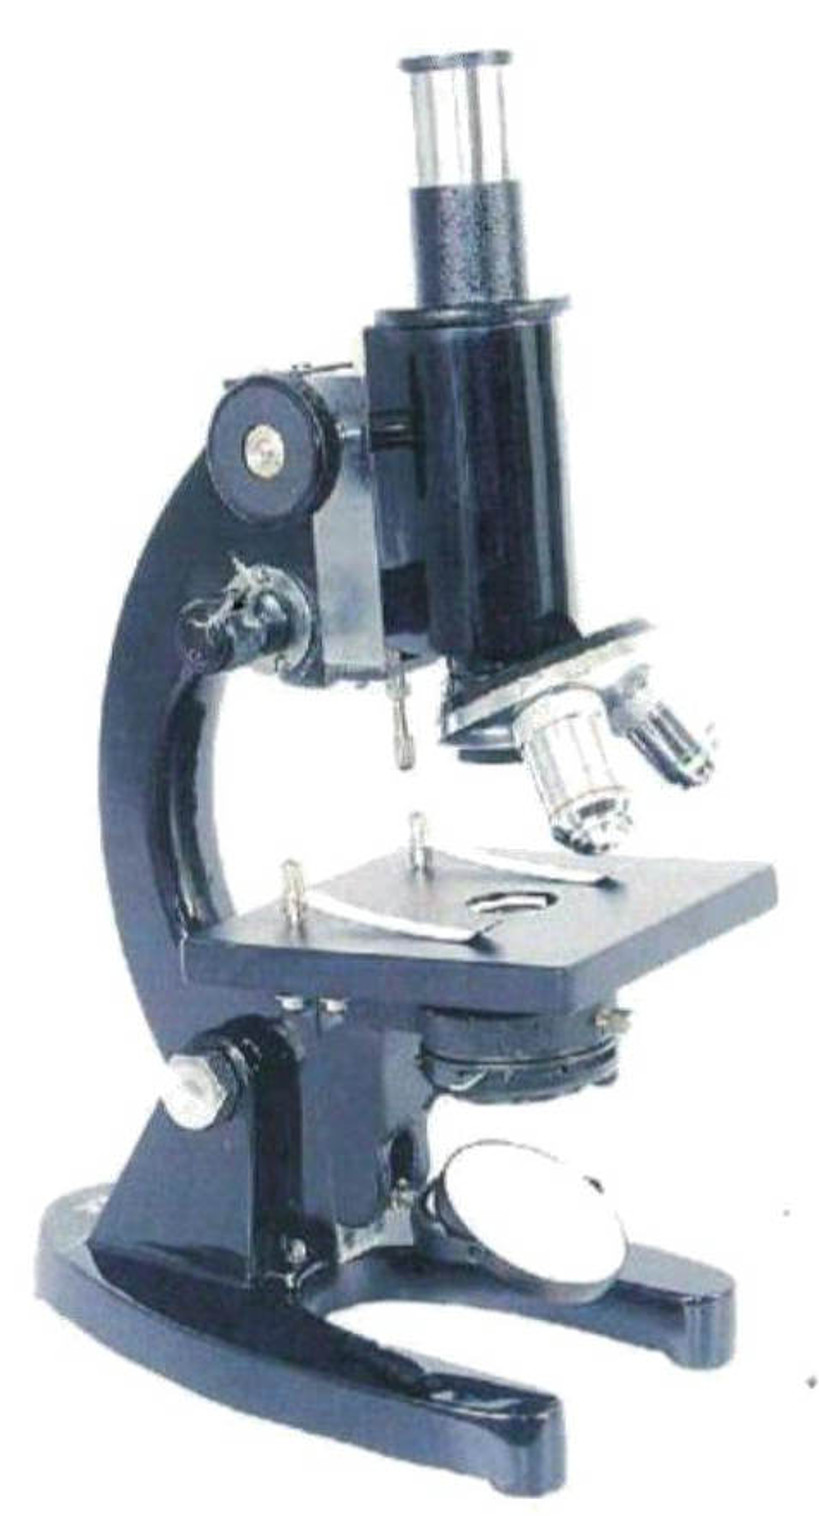
\includegraphics[scale=10]{./compoundMicroscope.jpg}
			\caption*{\textbf{Compound Microscope}}
			\label{compound microscope}
		\end{figure}
		}

		Physical terms:
		\begin{itemize}
			\item{Resolution \par It is the ability to reveal closely adjacent structural details as separate and distinct. The limit of magnification of a microscope is set by its resolving power.}
			\item{Numerical Aperture \par It is the ratio of the diameter of the lens to its focal length. Greater the numerical aperture greater the resolving power.}
			\item{Working Distance \par It is the distance between the objective lens and the slide.}
		\end{itemize}

		\section*{Parts Of The Microscope}

		\subsection*{Support System}
		\begin{enumerate}
			\item{Base \par It supports the microscope on the working table.}
			\item{Pillars \par Two upright pillars project upwards from the base.}
			\item{Handle \par Handle is hinged to the pillars. It supports the magnifying and adjusting systems. It is the handle by which the microscope must be carried. It is curved and the microscope can be tilted at the hinged joint.}
			\item{Body tube \par The eyepiece fits into the top of the body tube. The nose piece with the objective lenses fits into its lower end. It is the part through which the light passes to the eyepiece. It actually conducts the image.}
			\item{Stage \par Fixed stage is the horizontal platform on which the object is placed. It has a central opening through which the illuminating system focuses the light on the object. Mechanical stage has a spring mounted clip to hold the slide or counting chamber in position. It has two screws to move the mounted object from side to side and for ward and backwards.}
			\item {Nose piece \par Fixed nose piece is attached to lower end of body tube. Revolving nose piece carries objective lenses of different magnifying powers.}
		\end{enumerate}

		\subsection*{Adjusting System}
		It consists of the coarse and fine adjustment screws mounted in the handle by a double sided micrometer mechanism.
		\begin{enumerate}
			\item{Coarse adjustment screws \par It consists of rack and pinion which moves the tube rapidly through a large distance when the screw is rotated clockwise or anticlockwise. It is used to obtain an approximate focus of the object.}
			\item{Fine adjustment screws \par Similar to coarse adjustment screw, but several rotations will move the tube through a very small distance. It is used to obtain exact focus of the object.}
		\end{enumerate}

		\subsection*{Illumination System}
		\begin{enumerate}

			\item{Source of illumination \newline
				\par Light source may be internal or external.
				\par Internal source –In modern microscopes, there is an in-built light source with an electrical tungsten lamp, which is placed directly under the stage.
				\par External source – This can be from an electric lamp housed in a lamp box with a window or from the sun. The rays of light are reflected by a mirror towards the object. The mirror is located at the base of the microscope which is plain or concave.}
			\item{Condenser
				\par It focuses the rays of light reflected from the mirror onto the object under observation and helps in resolving the image. It is mounted below the stage of the microscope. Position of the condenser has to be adjusted according to the objective lens used.}
			\item{Iris diaphragm
				\par It is located at the bottom of the condenser. It has a central aperture. The size of the aperture can be altered to regulate the amount of light that passes through the condenser onto the object under observation.}
		\end{enumerate}

		\subsection*{Magnification System}
		\begin{enumerate}

			\item{Eye piece
				\par This is a magnifying lens inserted into the upper end of the body tube. Each eyepiece has two lenses, an eye lens mounted at the top and a field lens at the bottom. It has a magnification power of 5 and 10. It magnifies the primary image to give a virtual image which is observed through the eye piece.}
			\item{Objective lens

				\par Three objective lenses are fitted to the lower end of the body tube in the revolving nose piece. They are the low power, high power and oil immersion objective lenses. The desired objective lens is placed close to object on the stage and it produces a real magnified and inverted primary image. When the oil immersion objective is used, the space between the object and the lens is filled with cedar wood oil which has the same refractive index as that of glass and hence prevents refraction of light.\newline
				\begin{tabular}{c | c | c | c}
					\hline
					Objective & Working Distance & Numerical Aperture &Magnification\\
					\hline
					Low Power & 5 to 15 $mm$ & 0.3 & 10\\
					\hline
					High Power
					&0.5 to 4 $mm$
					&0.65
					&40/45 \\
					\hline

					%next row
					Oil immersion
					&0.15 to 1.5 $mm$
					&1.3
					&100 \\

					\hline





				\end{tabular}

				\par
				Adjustments for low power objective
				\begin{itemize}
					\item {Concave mirror is used.}
					\item {Condenser is lowered.}
					\item {Iris diaphragm is slightly opened to decrease the intensity of illumination.}
				\end{itemize}

				\par
				Adjustments for high power objective
				\begin{itemize}
					\item{Concave mirror is used.}

					\item{Condenser is slightly raised.}

					\item{Iris diaphragm is partially opened to increase the intensity of illumination.}
				\end{itemize}

				\par
				Adjustments for oil immersion objective (OPR)
				\begin{itemize}

					\item{Open the Iris diaphragm fully to get maximum intensity of illumination}

					\item{Plane mirror is used.}

					\item{Raise the Condenser.}
				\end{itemize}
				}




			\end{enumerate}

			\section*{Precautions}
			\begin{itemize}
				\item Objectives and eyepiece should be free from dust.
					item The mirror, the position of the condenser, and the aperture of the iris should be checked in order to get proper illumination.
				\item While changing the objective it should be noted that the objective clicks into its proper position.
				\item Do the necessary microscopic adjustments before using each objective.
				\item While focusing, lower the objective close to the slide and focus the object by slowly raising the objective.
				\item Never bring down the objective with the coarse adjustment screw while looking into the microscope.
				\item Examine the slide under low power and high power before examining it under oil immersion objective.
				\item After using oil immersion objective, clean the lens with filter paper and xylol.
			\end{itemize}

			\section*{Questions}
			\begin{enumerate}
				\item Name the oils used for oil immersion objective.
				\item How will you calculate the total magnification power of the microscope for each objective?
				\item Name the other types of microscope.
			\end{enumerate}
			%------}}}
			%-----------Hemocytometer----{{{

			\chapter*{\centering Hemocytometer}
\addcontentsline{toc}{chapter}{Hemocytometer}
			\begin{tabular}{p{5in} p{1in}}
				\textbf{Exp No:}  & \textbf{Date:}\\
			\end{tabular}

			\addfig{%
				\begin{figure}[h]
					\centering
					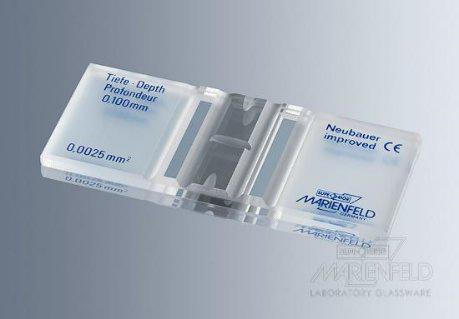
\includegraphics[scale=.5]{./neubar.jpg}
					\caption*{\textbf{Neubauer Chamber}}
					\vspace{1.5cm}
					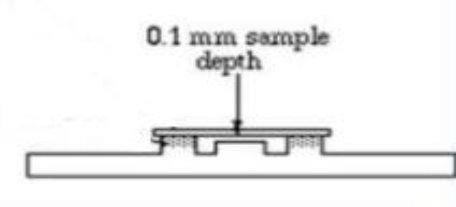
\includegraphics[scale=0.5]{./neubarSide.jpg}
					\caption*{\textbf{Neubauer Chamber - side view}}
					\vspace{2cm}
					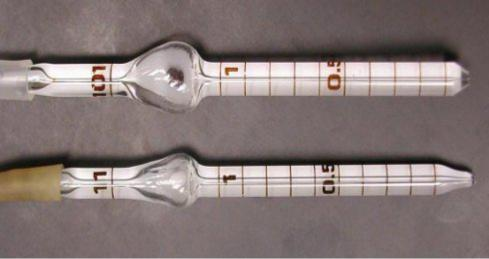
\includegraphics[scale=.5]{./pipette.jpg}
					\caption*{\textbf{RBC \& WBC pipettes}}
					\label{chamber}
				\end{figure}
				}
				\addfig{%
					\begin{figure}[h]
						\centering
						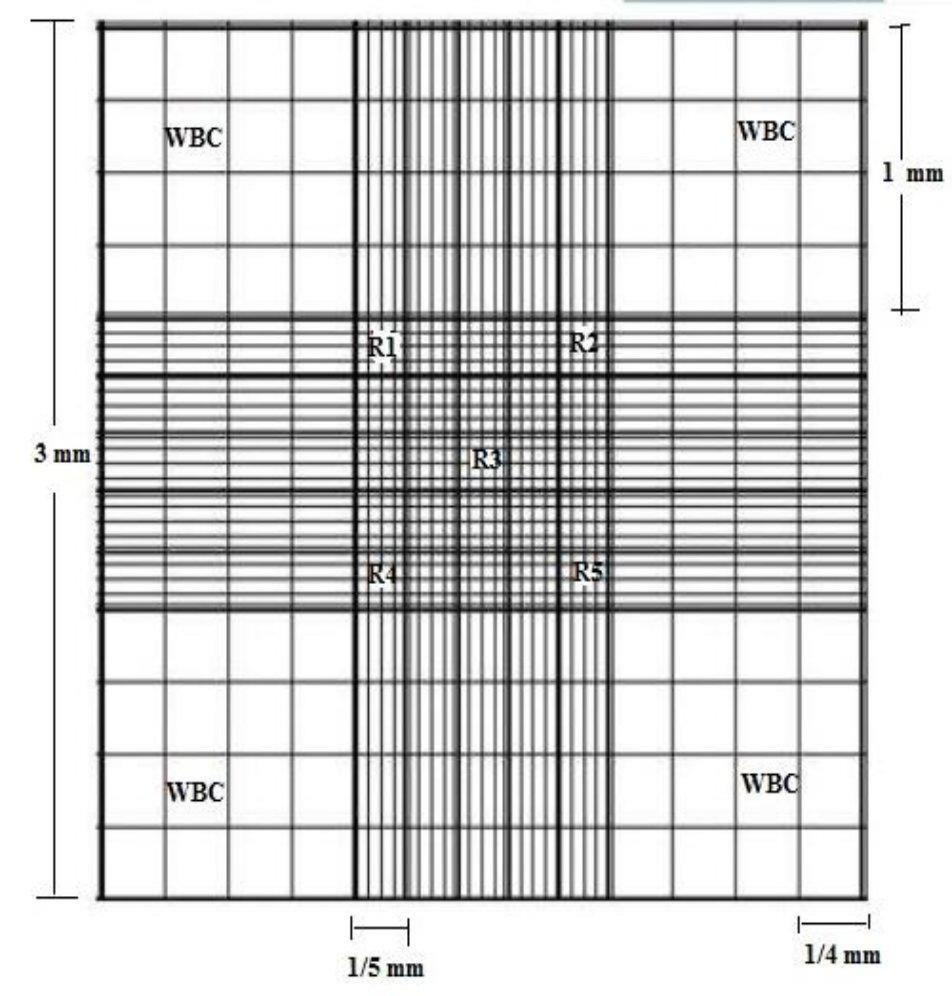
\includegraphics[scale=.5]{./grid.jpg}
						\caption*{\textbf{Neubauer Chamber's Counting Region}}
						\label{grid}
					\end{figure}
					}


					\section*{Introduction}
					The formed elements of blood are counted by Hemocytometry. The apparatus is called as hemocytometer. It consists of diluting pipettes and counting chamber.
					The counting chamber in common use is the improved Neubauer’s counting chamber. This is a thick glass slide divided into two central platforms by a ‘H’ shaped groove. The central platform is slightly lower than the sides. When a cover slip is placed over the central platforms, resting on the side platforms, a space of $\frac{1}{10}$  $mm$ depth will be present between the cover slip and the central platform. This area is used for charging the chamber with the diluted blood for cell counting.
					The central platforms have ruled squares which are used for cell counting. The ruled area is a square measuring 3 $mm$ $\times$ 3 $mm$. This area is divided into 9 large equal squares each having an area of 1 $mm$$^2$. The four large corner squares are used for WBC count. The central square is used for RBC count. All nine squares are used for Absolute eosinophil count.

					\section*{WBC counting squares}
					\begin{itemize}
						\item
							The four large corner squares are used for the WBC count and each has 16 medium squares (16$\times$4=64 medium squares).
						\item {
								Side of each large square is 1 $mm$.}
							\item{
									Area of each large square is 1 $\times$ 1 = 1 $mm$$^{2}$.}
								\item {
										Volume of each large square = area $\times$ depth = 1 $\times$ $\frac{1}{10}$ = $\frac{1}{10}$ $mm^3$.}
								\item{
										Volume of each medium square = $\frac{1}{4}$ $\times$ $\frac{1}{4}$ $\times$ $\frac{1}{10}$ = $\frac{1}{160}$ $mm^3$.}
					\end{itemize}

					\section*{RBC counting squares}
					\begin{itemize}

						\item{The 1$mm^2$ central RBC square is divided into 25 medium sized squares by triple lines. The four corner and central medium sized squares are used for RBC count.}
						\item{Each medium sized square is further divided into 16 small squares.}
						\item{(5 $\times$ 16 = 80 small squares).}
						\item{Side of each medium sized square is $\frac{1}{5}$ $mm$.}
						\item{Area of each medium sized square is $\frac{1}{5}$ $\times$ $\frac{1}{5}$ = $\frac{1}{25}$ $mm^2$.}
						\item{Volume of each medium sized square is $\frac{1}{250}$ $mm^3$.}
						\item{Volume of each smallest square = $\frac{1}{20}$ $\times$ $\frac{1}{20}$ $\times$ $\frac{1}{10}$ = $\frac{1}{4000}$ $mm^3$.}

					\end{itemize}

					\section*{Pipettes}
					The pipettes are used to dilute the blood to a known dilution.
					Two types of pipettes are used – RBC pipette, WBC pipette .
					\par


					Parts of a pipette are:-\newline
					\textbf{The Stem:}
					The long narrow stem has a capillary bore and a well-grounded conical tip. It is divided into 10 equal parts with two numbers etched on it – 0.5 in the middle and 1.0 at the junction of stem and the bulb.\newline
					\textbf{The bulb:}
					The bulb contains a free-rolling bead. The bead helps in identifying the pipette and mixing the diluents with blood in the bulb. Free rolling of the bead in the bulb indicates whether the pipette is dry or not.\newline
					\textbf{Rubber tube and mouthpiece:}
					The narrow rubber tube attached to the bulb, facilitates filling of the pipette by gentle suction. There is a marking just above the bulb. This marking is 11 in WBC C pipette and 101 in RBC pipette. The graduations do not indicate absolute or definite amounts in terms of cubic mm .They only indicate relative volumes in relation to each other. The markings indicate relative parts in the pipette\newline

					\subsection*{RBC pipette}
					\begin{itemize}

						\item{Markings are 0.5, 1.0 and 101}
						\item{The capillary bore is narrow}
						\item{Bulb is larger and has a red bead}
						\item{Volume of the bulb is 100 parts}
					\end{itemize}

					\subsection*{WBC pipette:}
					\begin{itemize}
						\item{Markings are 0.5, 1.0 and 11}
						\item{The capillary bore is wider}
						\item{Bulb is smaller and has a white bead}
						\item{Volume of the bulb is 10 parts}
					\end{itemize}


					\subsection*{Finger Prick}
					\begin{itemize}
						\item{Clean the tip of the finger with spirit and allow the area to dry.}
						\item{Prick the tip of finger with the lancet, deep enough to get a good drop of blood.}
						\item{Don’t squeeze the finger pulp after pricking as this leads to the seepage of tissue fluid resulting in dilution of the blood.}
						\item{The prick is usually made on middle or ring finger.}
					\end{itemize}

					\subsection*{Filling The Pipette}
					\begin{itemize}

						\item{Under aseptic precautions prick the finger and wipe away the first drop and allow the flowing blood to form a good sized drop.}
						\item{Hold the pipette horizontally and dip its end into the blood drop. Gently suck blood up-to 0.5 or 1.0 mark depending on the dilution required.}

						\item{If the blood overshoots 0.5 or 1.0 mark, remove the excess blood by gently tapping the tip of the pipette on to the palm. Do not use cotton or any absorbent material as it might absorb water content of blood and concentrates blood.}
						\item{Place the tip of the pipette into the diluting fluid and suck up-to the 11 mark in case of WBC pipette or 101 mark in case of RBC pipette without any air bubble.}
						\item{Place the pipette horizontally between the palms of both hands with the rubber tube folded parallel to it and roll the pipette for 1-2 minutes, for thorough mixing of blood with the fluid in the bulb.}

					\end{itemize}

					\subsection*{Precautions}
					\begin{itemize}

						\item{The pipette must be dry and free from clotted blood and the bead must roll freely in the bulb.}
						\item{The tip must not press against the finger or be lifted out of the blood drop or else air will enter it.}
						\item{The blood must be diluted immediately, or else it may clot.}
						\item{Always hold the pipette horizontally to avoid leakage of fluid from the pipette while mixing.}

					\end{itemize}


					\subsection*{Focusing The Counting Grid}
					\begin{itemize}

						\item{	Focus the counting grid with low power and then high power objective.}
						\item{	The lines of the squares must be seen clearly.}
					\end{itemize}

					\subsection*{Charging The Chamber}
					\begin{itemize}

						\item{	 Place the coverslip on the central platform of the chamber covering the ruled squares.}
						\item{	 Discard the stem fluid before charging the chamber as it contains only the diluting fluid.}
						\item{	 Form a good drop of diluted blood at the tip of the pipette, by squeezing the rubber tube, while closing its mouthpiece or by gently blowing through the rubber tube.}
						\item{	 Hold the pipette at 45 degree inclination and touch the chamber with the  tip of the pipette between the cover slip and the central platform.}
						\item{	 A thin layer of the fluid spreads under the coverslip on the central  platform by capillary action.}
						\item{	 Avoid overcharging the chamber which is recognized by fluid in the  trenches.}
						\item{	 Wait for 2 minutes for the cells to settle down.}
						\item{	 Focus  the  squares  under  the  desired  objective  and  start  counting.}
					\end{itemize}


					\subsection*{Precautions}
					\begin{itemize}

						\item{	 The chamber and the coverslip should be properly cleaned.}
						\item{	 The contents of the bulb must be thoroughly mixed before charging.}
						\item{	 2-3 drops of fluid must be discarded from the pipette before charging as the stem contains only diluents.}
						\item{	 Air bubbles should not enter the platform of the chamber while charging.}
						\item{	 The chamber should not be overcharged ( gives false low results) or undercharged ( the cells may not be found in peripheral squares).}
					\end{itemize}

					\subsection*{Cell Counting}
					\begin{itemize}

						\item{	 Count the cells in the respective squares.}
						\item{	 Care should be taken not to count the same cells again by following L rule. (Count the cells present inside the square and those on the left and lower lines. Ignore those on the right and upper lines).}
					\end{itemize}

					\subsection*{Questions}

					\begin{enumerate}

						\item{	 What are the other types of cell counting chambers ?}

						\item{	 What are the other cells that can be counted using Neubauer’s chamber?}
						\item{	 Mention the differences between RBC and WBC pipettes.}
					\end{enumerate}
					%-----------}}}
					%-------RBCcount---{{{
					\chapter*{\centering Estimation Of Total RBC Count}
\addcontentsline{toc}{chapter}{Estimation Of Total RBC Count}

					\begin{tabular}{p{5in} p{1in}}
						\textbf{Exp No:}  & \textbf{Date:}\\
					\end{tabular}

					\section*{Aim}

					To enumerate the number of  erythrocytes in 1 $mm^3$ of blood.
					\section*{Apparatus Required}
					Microscope, Hemocytometer (RBC diluting pipette and counting chamber), RBC diluting fluid (Hayem’s fluid), spirit, cotton and lancet.

					\section*{Hayem's Fluid - composition}
					\begin{itemize}

						\item{		Sodium chloride - 0.5 g	- Maintains isotonicity}
						\item{		Sodium bisulphate - 2.5 g - Prevents aggregation  of RBCs (Rouleaux formation)}
						\item{		Mercuric perchloride - 0.25 g - Acts  as preservative, antifungal and antibacterial}
						\item{		Distilled water - 100 ml - Acts as solvent}
					\end{itemize}


					\section*{Procedure}

					Make  a  sterile  finger  prick  and  discard  the  first drop  of blood. Draw blood up-to  0.5  mark  and  Hayem’s  fluid  up-to 101  mark  with  the  pipette. Mix  the contents thoroughly. Discard  the  first  few  drops and then charge  the  Neubauer chamber. Allow  the cells to  settle  for  3-4  minutes.Count the RBCs in the 4 medium sized corner squares and  in the central medium sized square of the RBC counting area (total of 16 x 5 = 80 smallest squares) under high power objective.


					\section*{Calculation}
					Number of RBCs in 5 medium sized RBC squares = n\newline\vspace{.4cm}
					Area of 1 medium  sized RBC square =$\frac{1}{5}$ $\times$ $\frac{1}{5}$ = $\frac{1}{25}$ $mm^2$\newline\vspace{.4cm}
					Volume of 1 medium sized RBC square = $\frac{1}{25}$ $\times$ $\frac{1}{10}$ = $\frac{1}{250}$ $mm^3$\newline\vspace{.4cm}
					Volume of 5 medium sized RBC squares = $\frac{1}{250}$ $\times$ 5= $\frac{1}{50}$ $mm^3$\newline\vspace{.4cm}
					Number of cells in  $\frac{1}{50}$ $mm^3$ of diluted blood  = n\newline\vspace{.4cm}
					Number of cells in  1 $mm^3$  of diluted blood = 50 n\newline\vspace{.4cm}
					Dilution factor = 1 : 200\newline\vspace{.4cm}
					Number of cells in 1 $mm^3$ of un diluted blood 	= n $\times$ 50 $\times$ 200  \newline\vspace{.4cm}

					\section*{Result}
					RBC  count in the given  blood sample is $\rule{5cm}{0.1cm}$ cells / $mm^3$
					\section*{Questions}
					\begin{enumerate}

						\item {Name the other diluting fluids used for red  cell count.}
						\item{How will you identify the RBC counting squares?}
						\item{What is the normal RBC count in males and females?}
						\item{Why is the RBC count high in males?}
						\item{Mention the physiological and pathological causes for anemia and polycythemia?}


					\end{enumerate}
					%-----------}}}
					%--------WBC count---{{{
					\chapter*{\centering Estimation Of Total WBC Count}
\addcontentsline{toc}{chapter}{Estimation Of Total WBC Count}

					\begin{tabular}{p{5in} p{1in}}
						\textbf{Exp No:}  & \textbf{Date:}\\
					\end{tabular}
					\section *{Aim}
					To enumerate the number of leucocytes (white blood cells) in 1 $mm^3$ of blood.
					\section*{Apparatus Required}
					Microscope, Hemocytometer, WBC pipette, Turk’s fluid, Spirit, Cotton, Lancet
					\section*{Turk's Fluid Composition}
					\begin{tabular}{l c l}

						1\% Glacial Acetic Acid	&	-&	1.5 ml - Lyses RBCs without affecting WBCs\\
						Gentian Violet&			-&	1.5 ml - Stains nuclei of WBCs\\
						Distilled Water&		-&	100 ml - Acts as solvent\\

					\end{tabular}
					\section*{Procedure}

					Make a sterile finger prick and discard the 1st drop of blood. Draw blood up-to 0.5 mark and Turk’s fluid up-to 11 mark in the WBC pipette. Mix the contents thoroughly. Discard the first few drops and charge the Neubauer chamber. Allow the cells to settle for 3 to 4 minutes. Count the WBCs in the 4 corner large squares (WBC counting area) under high power objective.

					\section*{Calculation}

					Number of cells in 4 WBC squares = n\newline\vspace{.2cm}
					Area of 1 WBC square = 	1$\times$ 1 	= 1 $mm^2$\newline\vspace{.2cm}
					Volume of 1 WBC square	= 1$\times$ $\frac{1}{10}$ = $\frac{1}{10}$ $mm^3$\newline\vspace{.2cm}
					Volume of 4 WBC squares =4$\times$ $\frac{1}{10}$ = $\frac{4}{10}$ $mm^3$\newline\vspace{.2cm}
					Number of cells in $\frac{4}{10}$ $mm^3$ of Diluted blood 	= n \newline\vspace{.2cm}
					Therefore, Number of cells in 1 $mm^3$ of Diluted blood = 	n $\times$ $\frac{10}{4}$\newline\vspace{.2cm}
					Dilution Factor = 1 : 20\newline\vspace{.2cm}
					Therefore, Number of cells in 1 $mm^3$ of Undiluted blood 	= n $\times$ $\frac{10}{4}$ $\times$ 20 =	n $\times$ 50\newline\vspace{.2cm}


					\section *{Result}

					WBC count in the given  blood sample is $\rule{5cm}{0.1cm}$ cells / $mm^3$

					\section*{Questions}


					\begin{enumerate}

						\item{What is the normal RBC : WBC ratio ?}
						\item{ In which condition is RBC pipette used for counting WBCs ?}
						\item{ Why is blood diluted only 20 times in WBC counting?}
						\item{ Mention the physiological and pathological causes of high and low WBC count.}
						\item{ What is Leucocytosis ?}
						\item{ What is Leukemia?}
					\end{enumerate}
					%----}}}
					%------AEC---{{{
					\chapter*{\centering Absolute Eosinophil Count}
\addcontentsline{toc}{chapter}{Absolute Eosinophil Count}

					\begin{tabular}{p{5in} p{1in}}
						\textbf{Exp No:}  & \textbf{Date:}\\
					\end{tabular}

					\section*{Aim}

					To determine the number of eosinophils per cu mm of blood
					\section*{Apparatus Required}
					Microscope, Hemocytometer, Dunger’s fluid, spirit, cotton and lancet.
					\section*{Dunger's Fluid Composition}
					1\% of solution of eosin in water (5$ml$)- Eosin stains the eosinophilic granules.\newline
					Acetone (5$ml$) - Acetone lyses the cell membrane of all other cells.\newline
					Distilled water (90$ml$) - Distilled water to make up to 100$ml$.Acts as solvent.\newline
					\section*{Procedure}
					Make a sterile finger prick and discard the first drop of blood. Draw blood up-to 1 and the Dunger’s fluid up-to mark 11 in a WBC pipette. Mix the contents thoroughly. Cover the pipette with a petri dish lined by moistened filter paper. Wait for 15 minutes. Discard the first few drops and charge the Neubauer chamber. The eosinophils are identified by the pinkish orange stained coarse granules in the cytoplasm. Count the Eosinophils in all the 9 large squares of the Neubauer chamber. Count within 30 minutes of charging .
					\section*{Calculation}
					Number of cells counted in 9 large squares				=	n\newline\vspace{.2cm}
					Area of 1 large square				=	1 $\times$ 1		=	1$mm^2$	\newline\vspace{.2cm}
					Volume of 1 large square				=	1 $\times$ $\frac{1}{10}$	=	$\frac{1}{10}$ $mm^3$\newline\vspace{.2cm}
					Volume of 9 large square				=	9 $\times$ $\frac{1}{10}$	=	$\frac{9}{10}$ $mm^3$\newline\vspace{.2cm}
					Number of cells in $\frac{9}{10}$ $mm^3$ of diluted blood				=	n\newline\vspace{.2cm}
					Number of cells in 1 $mm^3$ of diluted blood				=	n $\times$ $\frac{10}{9}$\newline\vspace{.2cm}
					Dilution factor								=	1:10\newline\vspace{.2cm}
					Therefore, number of cells in 1 $mm^3$ of undiluted blood		=	n$\times$$\frac{10}{9}$$\times$10
					=	n$\times$$\frac{100}{9}$
					\section*{Result}

					Absolute Eosinophil count in the given  blood sample is $\rule{5cm}{0.1cm}$ cells / $mm^3$

					\section*{Questions}
					\begin{enumerate}

						\item{What is the normal value of Absolute Eosinophil Count ?}
						\item{What is the difference between the Differential Count and the Absolute Eosinophil Count ?}
						\item{What are the other diluting fluids used for Absolute Eosinophil Count?}
						\item{What are the contents of eosinophilic granules ?}
						\item{What are the functions of eosinophils?}
						\item{What are eosinopenia and eosinophilia?}
					\end{enumerate}
					%-----}}}
					%-----DC{{{
					\chapter*{\centering Differential Count}
\addcontentsline{toc}{chapter}{Differential Count}
					\begin{tabular}{p{5in} p{1in}}
						\textbf{Exp No:}  & \textbf{Date:}\\
					\end{tabular}

					\section*{Aim}
					To determine the differential count of White Blood Cells.
					\section*{Apparatus Required}
					Grease free and dry glass slides, Leishman’s stain, distilled water, lancet, spirit, cotton.	
					\section*{Leishman's Stain Composition \& Functions}
					Methylene blue (basic) 	     -	Stains acidic granules in cytoplasm especially 						granules of basophils and Nuclei of leucocytes.\newline
					Eosin (acidic) 		     -	Stains cytoplasm, basic granules in 							cytoplasm, Hemoglobin of RBCs.\newline
					Acetone free methyl alcohol - 	Fixes the cells (Acetone free methyl alcohol 						is used as acetone is a lipid solvent that 		lyses cell membrane).\newline 

					\section*{Procedure}

					\addfig{%
						\begin{figure}[h]
							\centering
							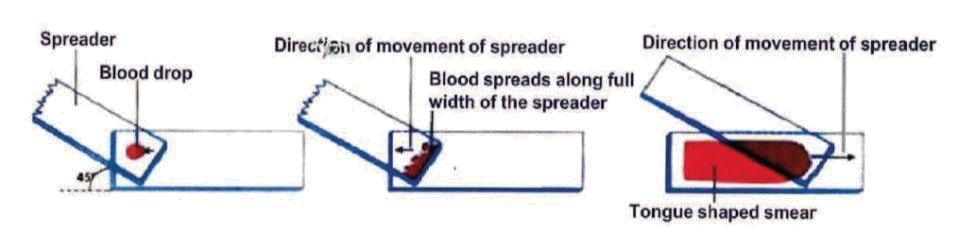
\includegraphics[scale=.50]{./smear1.jpg}
							\label{smear1}
							\vspace{3cm}
							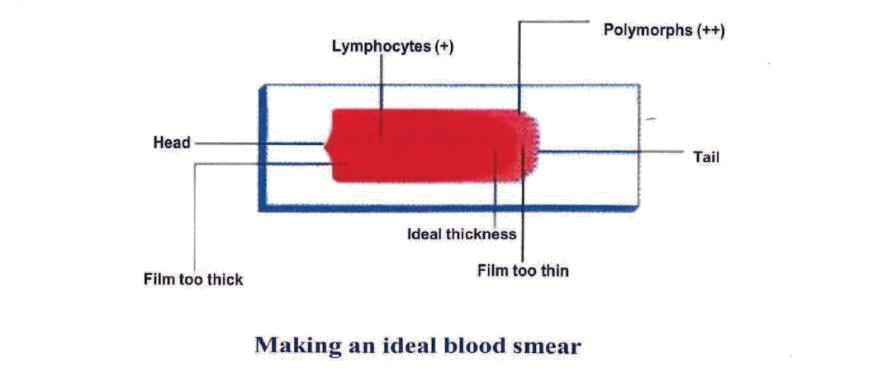
\includegraphics[scale=.50]{./smear2.jpg}
							\label{smear2}
							\vspace{1cm}
							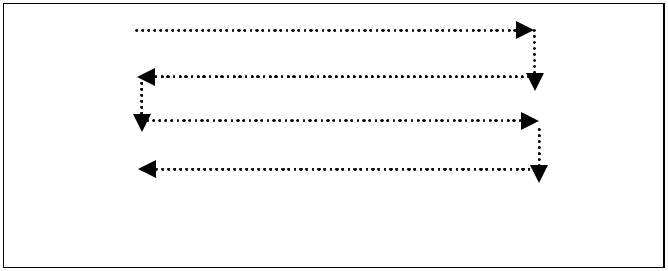
\includegraphics[scale=.50]{./smear3.jpg}
							\label{smear3}
						\end{figure}
						}
						Under aseptic precautions, prick the finger. Discard the first drop of blood. Place the slide on the table and support with left hand. Place the blood drop on the right end, one cm away from the edge. Place the spreader slide just in front of the blood drop. Draw the spreader slide backwards to touch the drop. The blood spreads across the edge of the spreader. Draw the spreader slide forward at an angle of 45$^{\circ}$ with a smooth, fast and firm movement to make a thin tongue shaped blood smear. Too thick, thin or a patchy smear is to be avoided. Air dry the smear quickly.

						Place the glass slide with the smear on a tray and add Leishman’s stain, drop by drop till the entire smear is covered with the stain. Count the number of drops added. Note the time and wait for 2 minutes (Fixation time). After 2 minutes, add double the quantity of distilled water over the film using a dropper. See to that the distilled water uniformly covers the entire surface of the slide and dilutes the stain homogeneously. Gently blow the stain and the distilled water from one end of the slide to the other for uniform mixing. Wait for about 8-10 minutes for the smear to take up the stain uniformly (Staining time).
						Flush the slide under a gentle stream of tap water to remove the excess stain. Dry the slide. Scan the film under low \& high power objective. Make necessary microscopic adjustments for oil immersion objective (100X). Add a drop of cedar wood oil over the smear at the junction between the body and the tail, as the smear will be of one cell thickness with uniform staining here. Cedar wood oil has the same refractive index as that of glass and minimizes refraction. Examine in a zig-zag manner as shown in the figure.

						Draw a table with 100 squares to count 100 WBCs and enter the type of cell as identified while examining the film.

						\addfig{%
							\begin{figure}[h]
								\centering
								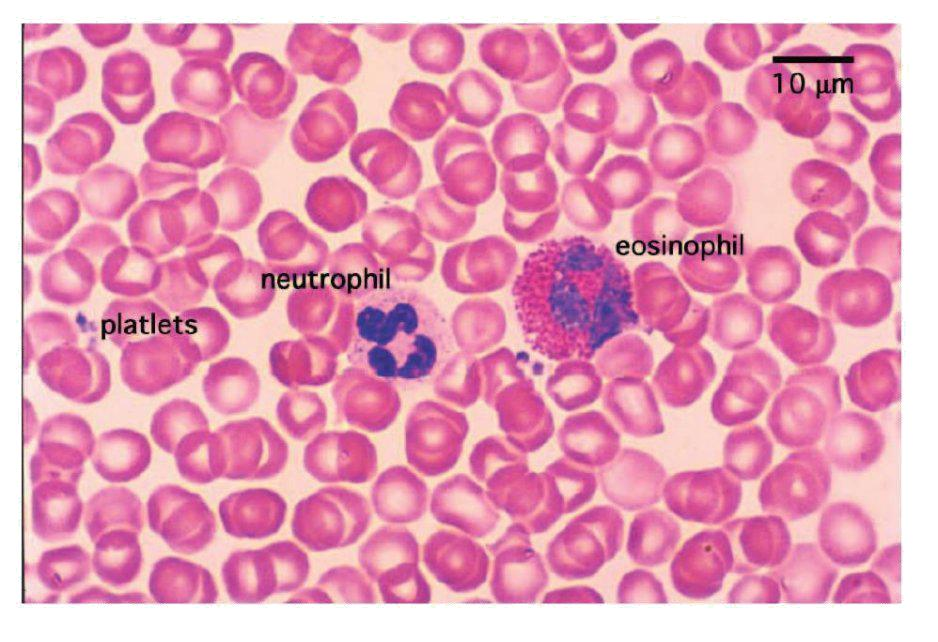
\includegraphics[scale=13]{./dc1.jpg}
								\label{dc1}
								\vspace{3cm}
								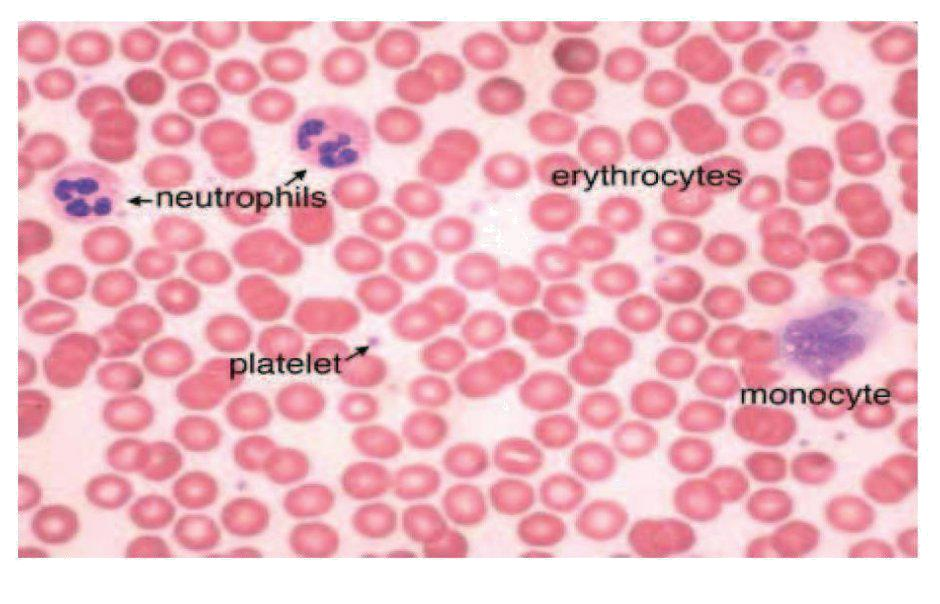
\includegraphics[scale=13]{./dc2.jpg}
								\label{dc2}
							\end{figure}
							}
							Under aseptic precautions, prick the finger. Discard the first drop of blood. Place the slide on the table and support with left hand. Place the blood drop on the right end, one cm away from the edge. Place the spreader slide just in front of the blood drop. Draw the spreader slide backwards to touch the drop. The blood spreads across the edge of the spreader. Draw the spreader slide forward at an angle of 45$^{\circ}$ with a smooth, fast and firm movement to make a thin tongue shaped blood smear. Too thick, thin or a patchy smear is to be avoided. Air dry the smear quickly.

							\section*{Result}
							The differential count of WBCs in the blood sample is as follows.\newline\vspace{.5cm}
							Neutrophil = $\rule{5cm}{0.1cm}$ \%\newline\vspace{.5cm}
							Eosinophil = $\rule{5cm}{0.1cm}$ \%\newline\vspace{.5cm}
							Basophil = $\rule{5cm}{0.1cm}$ \%\newline\vspace{.5cm}
							Lymphocyte = $\rule{5cm}{0.1cm}$ \%\newline\vspace{.5cm}
							Monocyte =$\rule{5cm}{0.1cm}$ \%

							\section*{Questions}
							\begin{enumerate}
								\item{Draw the different WBCs using appropriate colours.}
								\item{What other cells can you visualize in the smear?}
								\item{Enumerate the criteria of a good blood smear.}
								\item{Can tap water be used for dilution? why?}
								\item{Mention the functions of various types of WBCs and their abnormalities in count.}
								\item{Mention the clinical importance of peripheral blood smear.}
							\end{enumerate}

							\newpage

							\section*{Identifcation Of The Cells}
							A leukocyte is identified by its size, nucleus, cytoplasm and granules.
							\\
							\begin{center}
								\begin{tabularx}{\textwidth}{|*{5}{m{.2\textwidth}|X|}}
									%{|c|c|X|X|c|}
									\hline
									\textbf{Cell type}&
									\textbf{Size}&
									\textbf{Nucleus}&
									\textbf{Cytoplasm}&
									\textbf{Normal Values}\\

									\hline

									Neutrophil&
									10 – 14 ${\mu}m$&
									2-5 lobes connected by narrow strands of chromatin&
									Fine violet-pink granules&
									60-70\%\\

									\hline
									Eosinophil&
									10 - 15 ${\mu}m$&
									Often bi-lobed connected by thick strands of chromatin (spectacle shaped nucleus)&
									Coarse brick-red to orange granules&
									2-8\%\\
									\hline	

									Basophil&
									10 - 15 ${\mu}m$&
									Irregularly shaped (S shaped) nucleus masked by the granules&
									Very coarse deep purple granules&
									0-1\%\\
									\hline

									Small lymphocyte&
									7-9 ${\mu}m$&
									Single, round, almost fills the cell Thin crescent of clear, light blue cytoplasm. &
									No visible granules.&
									\multirow{2}{*}{20-30\%}\\
									\cline{1-4}

									Large lymphocyte&
									10 - 15 ${\mu}m$&
									Single, round, almost fills the cell.  May be central or eccentric.&
									Large crescent of clear, light blue cytoplasm. No visible granules.&
									\\
									\hline

									Monocyte&
									12 - 20 ${\mu}m$&
									Horse-shoe shaped nucleus Indented&
									Abundant, muddy blue in appearance. No visible granules.&
									1-5\%\\
									\hline
								\end{tabularx}	
							\end{center}
							%------}}}
							%---------Hb---{{{
							\chapter*{\centering Hemoglobin Estimation}
\addcontentsline{toc}{chapter}{Hemoglobin Estimation}
							\begin{tabular}{p{5in} p{1in}}
								\textbf{Exp No:}  & \textbf{Date:}\\
							\end{tabular}

							\section*{Aim}

							\addfig{%
								\begin{figure}[h]
									\centering
									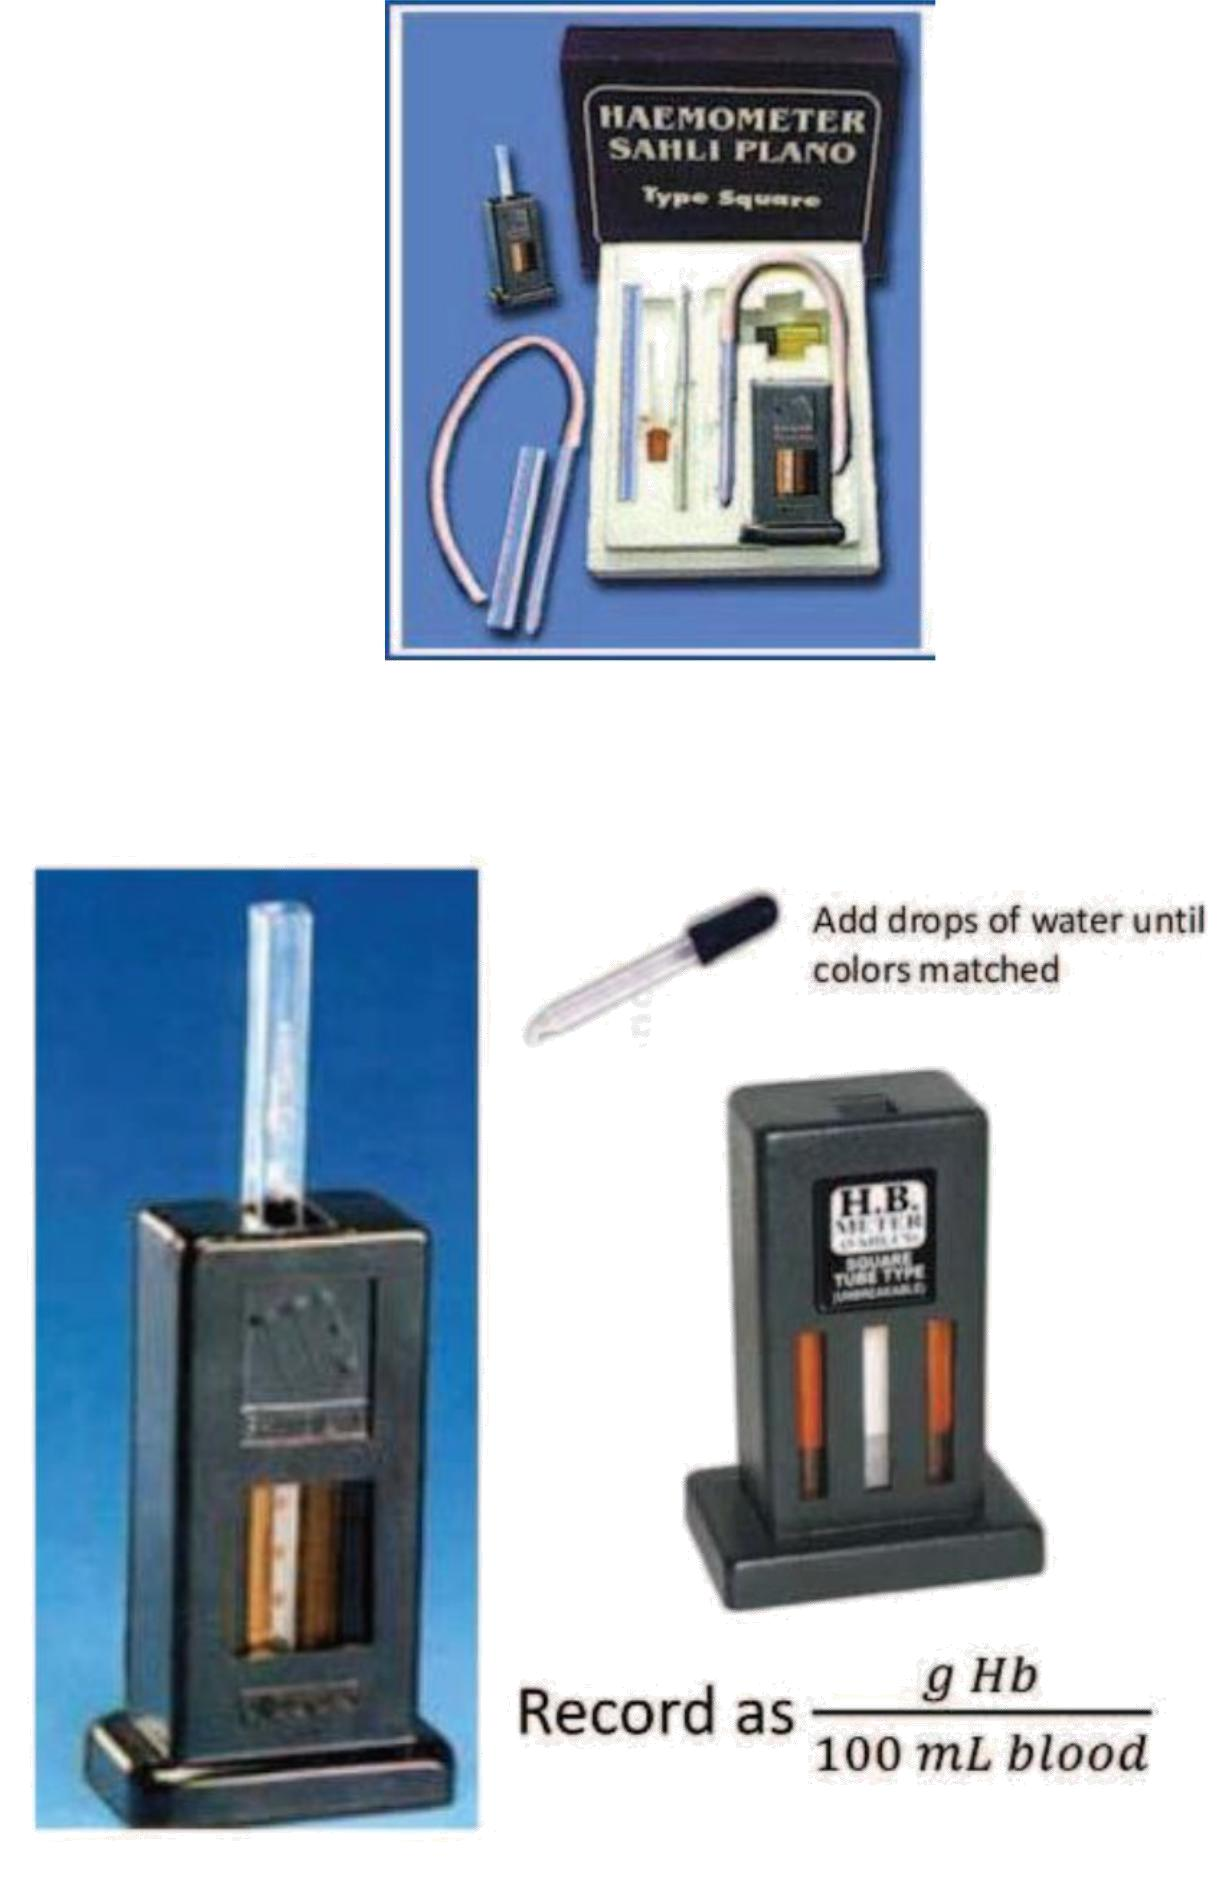
\includegraphics[scale=.25]{./hb.jpg}
									\label{hb}
									\caption*{\textbf{Sahli's Hemoglobinometer}}
								\end{figure}
								}
								To estimate the hemoglobin content of the blood by Sahli’s acid hematin method.
								\section*{Apparatus Required}
								Sahli’s Hemoglobinometer, Hemoglobin pipette, $\frac{N}{10}$ HCl, Distilled water, Glass stirrer, Dropper, Lancet, Spirit and Cotton.
								\section*{Principle}
								The amount of hemoglobin in the blood can be estimated by converting a known volume of blood into acid hematin solution and matching the color of the acid hematin solution with that of the standard colour.
								\section*{Description Of The Apparatus}
								The hemoglobinometer is a rectangular cubic box consisting of a central compartment to accommodate the ‘Hemoglobin tube’ and two yellow brown coloured cylindrical rods on either side as comparators. The Hb tube is graduated in percentage on one side and in gram percentage on the other side.

								The hemoglobin pipette has a single mark on the stem which corresponds to 0.02 ml or 20 cubic mm. A glass stirrer is provided for thorough mixing while diluting acid hematin solution.
								\section*{Procedure}
								\begin{enumerate}
									\item{Fill the hemoglobin tube with $\frac{N}{10}$ HCl up-to its lowest mark (2 $g$\%).}
									\item{Prick the finger under aseptic precautions to form an adequate drop of blood and suck blood into the hemoglobin pipette up-to 20 $mm^{3}$mark.}
									\item{Gently wipe exterior of the tip of the pipette.}
									\item{Insert the pipette into the hemoglobin tube containing $\frac{N}{10}$ HCl and blow out the blood. Rinse the pipette 2 or 3 times with the acid present in the tube.}
									\item{Wait for 10 minutes for the formation of acid hematin.}
									\item{Then, dilute the acid hematin by adding distilled water drop by drop and mix with the stirrer.}
									\item{Continue dilution till its color matches with that of the standards on either side.}
									\item{While matching, always take care to raise the stirrer above the level of the solution. Never take the stirrer out of the tube.}
									\item{Note down the final reading. (Lower meniscus).}
								\end{enumerate}
								\section*{Result}
								The Hb content of the given sample of blood is $\rule{5cm}{0.1cm}$ $g$\%
								\section*{Questions}
								\begin{enumerate}
									\item{What are the other methods used to estimate Hb content of blood?}
									\item{Which is the most reliable method for estimation of Hb?}
									\item{What are the different types of normal Hb in adults?}
									\item{Mention the names of abnormal hemoglobin.}
									\item{What are the differences between adult Hb \& fetal Hb?}
									\item{What are the different RBC indices? What are their clinical significance?}
								\end{enumerate}
								%-----}}}
								%-------BloodGrouping---{{{

								\chapter*{\centering Blood Grouping \& Typing}
\addcontentsline{toc}{chapter}{Blood Grouping \& Typing}
								\begin{tabular}{p{5in} p{1in}}
									\textbf{Exp No:}  & \textbf{Date:}\\
								\end{tabular}

								\section*{Aim}

								\addfig{%
									\begin{figure}[h]
										\centering
										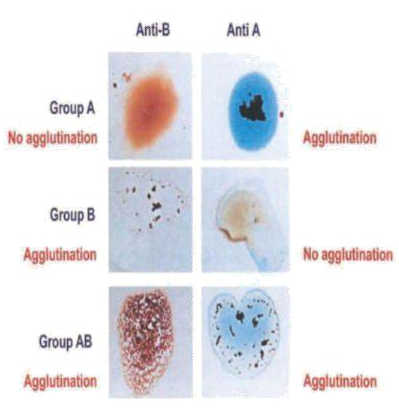
\includegraphics[scale=1.2]{./bloodGrouping.jpg}
										\label{bloodGrouping}
										\caption*{\textbf{Blood Groups Showing Agglutination}}
									\end{figure}
									}
									To determine the ABO blood group and Rh type of the given blood sample.
									\section*{Apparatus Required}
									Lancet, spirit, cotton, normal saline, clean white porcelain tile, glass marking pencil, anti-A serum, anti-B serum, anti-D serum, small sticks for mixing, glass slides, microscope.
									\section*{Principle}
									Determination of blood group is done by using specific agglutinins (antibodies), to confirm the presence or absence of corresponding agglutinogen (antigens) on the surface of the red blood cells.
									\section*{Procedure}
									\begin{enumerate}
										\item{Divide the porcelain tile into four columns with a marking pencil.}
										\item{Mark the columns as A, B, Rh and Control}
										\item{Take1ml of normal saline in a test tube.}
										\item{Prick the finger with the lancet under aseptic conditions.}
										\item{Mix 3-5 drops of blood with the saline to obtain a suspension of red blood cells.}
										\item{Add a drop each of anti-A, anti-B, anti-D sera and saline to the respective columns.}
										\item{Place a drop of the red cell suspension adjacent to the anti-sera in the respective columns.}
										\item{Mix the anti-sera and red cell suspension by using separate sticks.}
										\item{Wait for few minutes and observe the agglutination (clumping).}
										\item{Compare it with the saline standard.}
										\item{Record your findings.}
										\item{If there is doubt regarding agglutination, confirm it under the microscope.}
									\end{enumerate}
									\section*{Result}
									The blood group of the subject is $\rule{5cm}{0.1cm}$
									\section*{Questions}
									\begin{enumerate}
										\item{State Landsteiner’s law.}
										\item{What is cross-matching of blood?}
										\item{What is the preservative used to store blood in the blood bank?}
										\item{What are the clinical applications of blood grouping and Rh typing?}
										\item{What are the minor blood groups?}
										\item{What is the concept of universal donor/ universal recipient?}
										\item{What are the indications and hazards of blood transfusion?}
										\item{What are the differences between ABO system and Rh system?}
									\end{enumerate}
									%---------------}}}
									%----BleedingTime---{{{

									\chapter*{\centering Estimation Of Bleeding Time}
\addcontentsline{toc}{chapter}{Estimation Of Bleeding Time}
									\begin{tabular}{p{5in} p{1in}}
										\textbf{Exp No:}  & \textbf{Date:}\\
									\end{tabular}
									\addfig{%
										\begin{figure}[h]
											\centering
											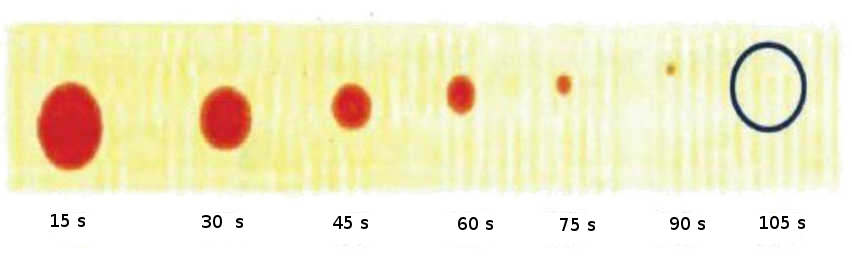
\includegraphics[scale=.5]{./bleedingTime.jpg}
											\label{bleedingTime}
											\caption*{\textbf{Estimation Of Bleeding Time}}
										\end{figure}
										}

										\section*{Aim}
										To determine the bleeding time by Duke’s method
										\section*{Apparatus Required}
										Filter paper, lancet, spirit, cotton swabs \& stop watch.	
										\section*{Principle}
										The time interval between skin puncture and spontaneous, unassisted stoppage of bleeding is called bleeding time. It is a test for assessing the function of platelets and integrity of capillaries.
										\section*{Procedure}
										\begin{enumerate}
											\item{Clean the tip of the finger with spirit and cotton and allow the finger to dry.}
											\item{Make a good deep finger prick with the lancet to get free flowing blood.}
											\item{Do not squeeze the finger.}
											\item{Immediately start the stopwatch.}
											\item{Gently touch the puncture site with a clean filter paper every 15 seconds.}
											\item{Repeat this step until no further blood spot appears on the filter paper.}
											\item{Observe that successive spots are smaller in size.}
											\item{Count the number of blood spots including the dry spot on the filter paper and divide it by 2 to get the bleeding time in minutes.}
											\item{Normal bleeding time by Duke’s method is 2-5minutes.}
										\end{enumerate}
										\section*{Result}
										The bleeding time determined by Duke’s method is $\rule{5cm}{0.1cm}$
										\section*{Questions}
										\begin{enumerate}
											\item{Define bleeding time.}
											\item{What are the other methods to determine the bleeding time?}
											\item{What is hemostasis?}
											\item{What is the role of platelets in hemostasis?}
											\item{What is the normal platelet count? What do you mean by thrombocytosis?}
											\item{Name few conditions where bleeding time is prolonged?}
											\item{What is Thrombocytopenic purpura? Comment on the clotting time in this condition.}
										\end{enumerate}
										%------------------------}}}
										%------------ClottingTime---{{{
										\chapter*{\centering Estimation Of Clotting Time}
\addcontentsline{toc}{chapter}{Estimation Of Clotting Time}
										\begin{tabular}{p{5in} p{1in}}
											\textbf{Exp No:}  & \textbf{Date:}\\
										\end{tabular}
										\section*{Aim}

										\addfig{%
											\begin{figure}[h]
												\centering
												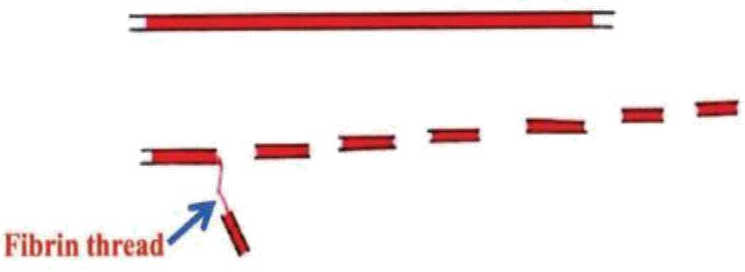
\includegraphics[scale=.5]{./clottingTime.jpg}
												\label{clottingTime}
												\caption*{\textbf{Estimation Of Clotting Time}}
											\end{figure}
											}
											To determine the clotting time of blood by Wright’s capillary glass tube method.
											\section*{Apparatus Required}
											Capillary glass tube, lancet, spirit, cotton swabs \& stop watch.
											\section*{Principle}
											When blood comes in contact with glass surface, the coagulation pathway gets activated.
											The time taken for the formation of insoluble fibrin thread(blood clot) is called clotting time.
											\section*{Procedure}
											\begin{enumerate}
												\item{Clean the tip of the ring finger with spirit and allow the finger to dry.}
												\item{Make a good deep finger prick with the lancet to get free flowing blood.}
												\item{Do not squeeze the finger.}
												\item{When a blood drop of optimum size has formed, gently place the end of the capillary tube in the drop such that the other end of the tube is at a lower level.}
												\item{Blood enters readily into the tube by capillary action.}
												\item{Start the stop watch.}
												\item{Hold the capillary tube with blood between the palms to maintain it at body temperature.}
												\item{After 2 minutes, break a small bit of capillary tube at its end and check for the formation of fibrin thread.}
												\item{Repeat it every 30 seconds until the appearance of insoluble fibrin thread between the broken ends of capillary tube and note the time.}
												\item{The appearance of the fibrin thread indicates that the blood has clotted.}
												\item{The total time taken for the formation of fibrin thread is recorded as the clotting time.}
												\item{Normal clotting time by this method is 2-8 minutes.}
											\end{enumerate}
											\section*{Result}

											The clotting time determined by Wright's capillary glass is $\rule{5cm}{0.1cm}$
											\section*{Questions}
											\begin{enumerate}
												\item{Define clotting time.}
												\item{What are the other methods used to determine the clotting time?}
												\item{Name the conditions in which clotting time is prolonged.}
												\item{What is haemophilia? Comment on the clotting time in this condition.}
												\item{What is clot retraction time?}
												\item{Name the Vitamin K dependent coagulation factors.}
												\item{What is an anticoagulant? Mention some invivo and invitro anticoagulants.}
												\item{Name the proteins involved in fibrinolytic system.}
											\end{enumerate}
											%--------}}}
											%-----ESR------{{{

											\chapter*{\centering Estimation Of Erythrocyte Sedimentation Rate}
\addcontentsline{toc}{chapter}{Estimation Of Erythrocyte Sedimentation Rate}
											\begin{tabular}{p{5in} p{1in}}
												\textbf{Exp No:}  & \textbf{Date:}\\
											\end{tabular}
											\section*{Aim}
											To determine the Erythrocyte Sedimentation Rate of the given blood sample.
											\section*{Apparatus Required}

											\addfig{%
												\begin{figure}[h]
													\centering
													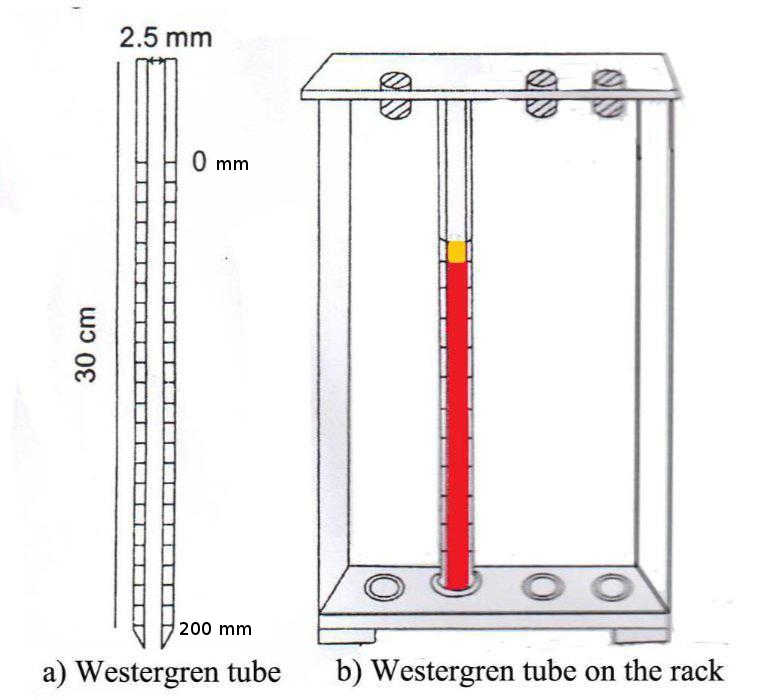
\includegraphics[scale=.5]{./esr.jpg}
													\label{esr}
													%\caption*{\textbf{Estimation Of Clotting Time}}
												\end{figure}
												}
												Westergren’s pipette and stand, syringe with needle and 3.8\% sodium citrate solution (anticoagulant)

												\section*{Principle}
												If blood treated with anticoagulant is allowed to stand in a tube placed vertically, the RBCs settle down gradually to the bottom since their specific gravity (1.093) is greater than that of the plasma (1.030).
												The rate  at  which the  RBCs settle down is called as Erythrocyte Sedimentation
												Rate.

												\section*{Procedure}
												\textbf{Westergren’s method:}\newline
												\begin{enumerate}	
													\item{Westergren’s pipette (tube) which is used for this procedure is open at both ends and is graduated in $mm$ from 0-200 with a bore diameter of 2.5$mm$.}
													\item{A sterile solution of 3.8\% sodium citrate is used as an anticoagulant.}
													\item{In a clean dry syringe, draw 2ml of blood from the antecubital vein under aseptic precautions and mix with 0.4ml of 3.8\% sodium citrate solution in a plastic  container with its lid closed.}
													\item{Fill the Westergren’s pipette with blood by sucking, after placing the tip of the finger over the top of the pipette to control the flow of blood into and out of it, or with a rubber bulb.}
													\item{Bring the blood column to exact zero mark.}
													\item{Keeping the finger (or the rubber bulb) over the pipette, transfer it to the Westergren stand by firmly pressing its lower end into the rubber cushion. Now.}
													\item{slip the upper end of the pipette under the screw cap.}
													\item{After an hour, note the $mm$ of clear plasma above the red cells.}
												\end{enumerate}
												\section*{Result}
												Erythrocyte Sedimentation Rate of the given blood sample is $\rule{5cm}{0.1cm}$ $mm$ in first hour.
												\section*{Questions}
												\begin{enumerate}
													\item{What is ESR?}
													\item{What are the 3 stages by which sedimentation of red cells occur?}
													\item{What are the other methods of estimating ESR?}
													\item{What are the advantages and disadvantages of Westergren method?}
													\item{What are the advantages and disadvantages of Wintrobe method?}
													\item{Can you use oxalate mixture in Westergren method and citrate in Wintrobe method?}
													\item{What are the factors determining ESR?}
													\item{What is rouleaux formation?}
													\item{Why is ESR reading taken after one hour?}
													\item{What is the normal ESR in males and females?}
													\item{Why is the ESR higher in females than that of males?}
													\item{What is the clinical significance of ESR?}
													\item{Mention some physiological and pathological conditions in which ESR is increased / decreased?}
													\item{What is zeta potential?}
												\end{enumerate}
												%------------------------}}}
												%---PackedCellVolume-{{{

												\chapter*{\centering Packed Cell Volume}
\addcontentsline{toc}{chapter}{Packed Cell Volume}
												\begin{tabular}{p{5in} p{1in}}
													\textbf{Exp No:}  & \textbf{Date:}\\
												\end{tabular}

												\section*{Aim}

												\addfig{%
													\begin{figure}[h]
														\centering
														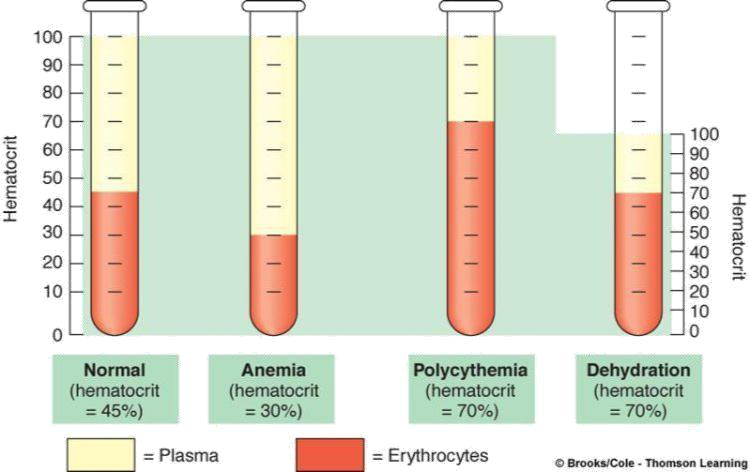
\includegraphics[scale=.5]{./pcv.jpg}
														\label{pcv}
														\caption*{\textbf{Estimation Of Packed Cell Volume }}
													\end{figure}
													}
													To determine the packed cell volume of the given blood sample.
													\section*{Apparatus Required}
													Centrifuge, Hematocrit tube (Wintrobe tube), Pasteur pipette, syringe with needle and double oxalate or EDTA (anticoagulant).
													\section*{Principle}
													When the blood is mixed with an anticoagulant and centrifuged in a hematocrit tube, the red blood corpuscles settle down at the bottom. The ratio of the volume of the settled red blood cells to that of whole blood in the hematocrit tube is called the packed cell volume or the hematocrit. A thin grey-white layer of white cells at the top of the red blood cell column is called the buffy coat layer.
													Hematocrit measures the percentage of volume of the packed red cells. It is used to diagnose and classify the various types of anemia, along with other red blood cell indices.
													\section*{Procedure}
													\textbf{Wintrobe's Method:}\newline
													\begin{enumerate}
														\item{Wintrobe’s tube is a thick walled cylindrical tube, 11$cm$ in length with an internal bore of 3$mm$. The tube is graduated from 0 to 10$cm$(100 $mm$) both in the ascending and descending order on either sides. The marking 0 – 10 from above downwards is used for ESR and the marking 0-10 from below upwards is used for reading PCV.}
														\item{In a clean dry syringe, 2ml of blood is drawn from the antecubital vein under aseptic precautions and transferred to a container with anticoagulant.}
														\item{The anticoagulated blood is then filled in the hematocrit tube from below upwards upto the mark 10 using the Pasteur pipette.}
														\item{The tube is centrifuged at a rate of 3000 rpm for a period of 30 minutes.}
														\item{At the end of 30 minutes, take the reading of upper level of packed red cell column.}
													\end{enumerate}
													\section*{Result}
													The packed cell volume or the hematocrit value of the given blood sample is $\rule{2cm}{.1cm}$\%
													\section*{Questions}
													\begin{enumerate}
														\item{Define PCV.}
														\item{What is the clinical significance of PCV?}
														\item{What is the normal range of PCV in males and females?}
														\item{What is the ideal anti-coagulant used and why?}
														\item{What is the difference between arterial and venous blood hematocrit?}
													\end{enumerate}
													%-----------------}}}
													%---------OsmoticFragility---{{{
													\chapter*{\centering Osmotic Fragility}
\addcontentsline{toc}{chapter}{Osmotic Fragility}
													\begin{tabular}{p{5in} p{1in}}
														\textbf{Exp No:}  & \textbf{Date:}\\
													\end{tabular}

													\section*{Aim}

													\addfig{%
														\begin{figure}[h]
															\centering
															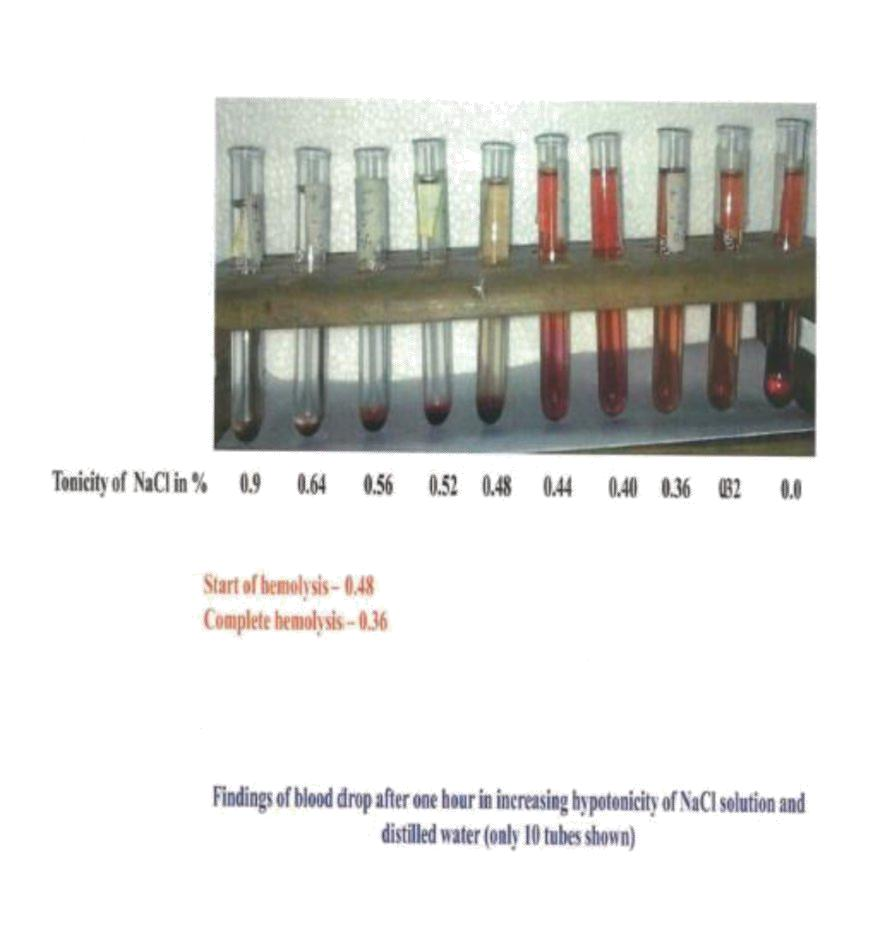
\includegraphics[scale=.5]{./osmoticFragility.jpg}
															\label{osmoticFragility}
															\caption*{\textbf{Estimation Of Osmotic Fragility}}
														\end{figure}
														}
														To determine the osmotic fragility of red blood cells in the given sample of blood.
														\section*{Apparatus Required}
														Test tubes with rack, anticoagulated blood, NaCl, distilled water.
														\section*{Principle}
														The normal red blood cells can remain suspended in 0.9\% sodium chloride solution (normal saline) for hours without any change in their size \& shape. But when they are placed in decreasing strengths of hypotonic sodium chloride solutions they imbibe water due to osmosis and finally burst releasing the hemoglobin pigment in the medium.
														\section*{Procedure}
														\begin{enumerate}
															\item{Sodium chloride solution of 1\% tonicity is prepared by dissolving 1 gram of NaCl in 100ml of distilled water.}
															\item{Arrange the test tubes in the rack and number them serially from 1 to 12.}
															\item{Prepare solutions of increasing hypotonicity by mixing required number of drops of 1\% NaCl solution and distilled water in the test tubes as given in the table.}
															\item{Use separate droppers for saline solution and distilled water.}
															\item{Note that the tube No.1 contains normal saline (0.9\% approximately) – Isotonic with plasma while tube No.12 contains distilled water.}
															\item{Draw 2ml of venous blood and treat it with anticoagulant in a test tube.}
															\item{Add one drop of blood into each of the above 12 tubes.}
															\item{Invert each tube gently once to mix blood with saline.}
															\item{Leave the test tubes undisturbed for one hour. Then observe the extent of hemolysis in each tube by holding the rack at eye level, with a white paper sheet behind it.}
														\end{enumerate}

														\begin{center}
															\csvautotabular{./osmoticFragility.csv}
														\end{center}
														\section*{Interpretation}

														\begin{itemize}
															\item{Test tube with partial hemolysis shows a supernatant fluid with pink colour proportionate to the degree of hemolysis and a lower layer of sedimented red cells at the bottom of the tube.}
															\item{Test tube with complete hemolysis shows a clear homogeneously pink solution with no cells at the bottom.}
															\item{Test tube with no hemolysis shows a clear colourless supernatant solution with a layer of sedimented red cells at the bottom of the tube}
														\end{itemize}
														\section*{Result}
														Hemolysis begins in $\rule{4cm}{.1cm}$\% of NaCl solution.\newline
														Hemolysis is complete in $\rule{4cm}{.1cm}$\% of NaCl solution.
														\section*{Questions}
														\begin{enumerate}
															\item{What is the normal range of osmotic fragility of red cells?}
															\item{What is osmosis?}
															\item{What do you mean by hypo/hyper tonicity?}
															\item{Define fragility.}
															\item{What happens to red cells when they are placed in isotonic, hypotonic and hypertonic solutions?}
															\item{Name some conditions which increase / decrease the osmotic fragility of the RBC.}
															\item{What are the advantages of the shape of red blood cells?}
														\end{enumerate}	
														%----------------------------}}}
														%--------------------------------SpecificGravity------------------------------{{{


														\chapter*{\centering Specific Gravity}
\addcontentsline{toc}{chapter}{Specific Gravity}
\addtocontents{toc}{\protect\newpage}

														\begin{tabular}{p{5in} p{1in}}
															\textbf{Exp No:}  & \textbf{Date:}\\
														\end{tabular}

														\section*{Aim}
														To determine the specific gravity of the given blood sample by using “Copper sulphate falling drop method”.

														\section*{Apparatus Required}

														\addfig{%
															\begin{figure}[h]
																\centering
																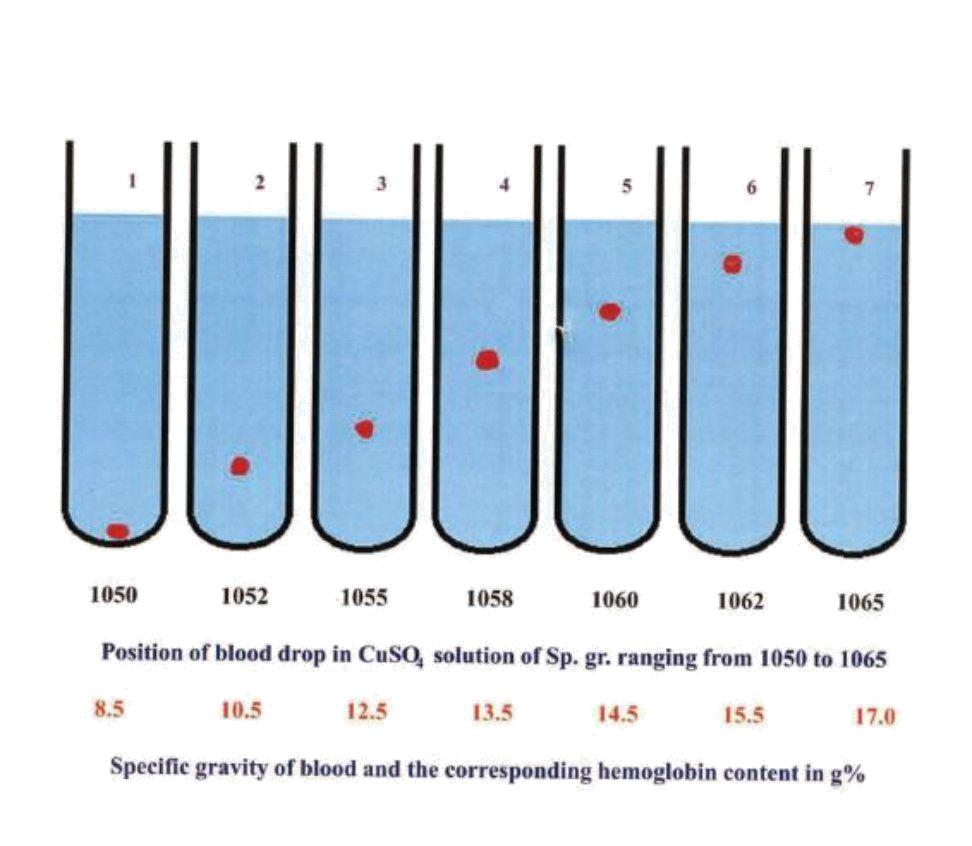
\includegraphics[scale=.5]{./specificGravity.jpg}
																\label{specificGravity}
																\caption*{\textbf{Determination Of Specific Gravity}}
															\end{figure}
															}
															Test tubes with rack, distilled water, anticoagulated blood, copper sulphate crystals (CuSO$_4$.5H$_2$O), beaker, measuring jar, Pasteur pipette
															\section*{Principle}
															The specific gravity of blood is determined by comparing the specific gravity of one drop of blood with that of copper sulphate solution of known specific gravity.
															\section*{Procedure}
															\begin{enumerate}
																\item{Stock solution of copper sulphate is prepared by dissolving 159 $g$ of CuSO$_4$.5H$_2$O in 1 liter of distilled water. The specific gravity of this stock solution is 1100.}
																\item{Standard copper sulphate solutions of known specific gravity are prepared by mixing specific quantity of stock solution and distilled water as shown in table and label the test tubes.}
																\item{Arrange the test tubes in rack in order of increasing specific gravity from left to right in test tube rack.}
																\item{Draw 2ml of venous blood and treat it with the anticoagulant in a test tube.}
																\item{Using Pasteur pipette a drop of blood is delivered into the middle test tube (no.4) from a height of about 1$cm$ above the surface of the copper sulphate solution so that it doesn’t touch the walls of the test tube.}
																\item{The drop sinks to about 2-3$cm$, and loses its momentum in 3-4 seconds. The drop then behaves according to its specific gravity; observe its behaviour during the next 15 seconds.}
																\item{If the specific gravity of blood drop is greater than that of the solution, the drop sinks to the bottom; if it is less than that of the solution, it rises to the surface and if it is the same as that of the solution, it becomes stationary and floats in the middle of the solution.}
																\item{If the drop continues to sink in test tube no.4, try with higher specific gravity solution; if it begins to rise, try with the lower specific gravity solution till you come to a solution where the drop remains in the middle of the solution.}
																\item{The whole observation has to be made in each step within 15 seconds.}
																\item{The tube in which the blood drop remains suspended in the middle of the tube for at least 15 seconds is noted and the specific gravity mentioned on the tube is read and recorded.}

															\end{enumerate}
															\begin{center}
																\csvautotabular{./specificGravity.csv}
															\end{center}
															\section*{Result}
															The specific gravity of the given blood sample is $\rule{4cm}{.1cm}$.
															\section*{Questions}
															\begin{enumerate}
																\item{Define specific gravity.}
																\item{What is the normal specific gravity of blood, plasma, serum and red blood cells?}
																\item{Why is copper sulphate solution used in this experiment?}
																\item{Why should the observation be made within 15 seconds?}
																\item{Enlist the physiological and pathological conditions in which the specific gravity of blood is increased and decreased.}
																\item{What are the clinical applications of this method? }
															\end{enumerate}
															%----------------------------------------------------------------------------}}}
															%-----------}}}
															\part*{Clinical Physiology}
%---------------GeneralExamination---{{{
															\chapter*{\centering General Examination}
\addcontentsline{toc}{chapter}{General Examination}

															\begin{tabular}{p{5in} p{1in}}
																\textbf{Exp No:}  & \textbf{Date:}\\
															\end{tabular}
															A thorough general examination is done before any systemic examination. Vital information such as name, age, sex, height, weight, occupation and address of the individual are recorded. The subject is comfortably seated. The room is well illuminated. It is always preferable to examine under good day light. The examiner should always be on the right side of the subject while examining.
															\section*{The following observations are recorded:}
															\section*{Level Of Consciousness}
														\addfig{%
															\begin{figure}[h]
																\begin{subfigure}[t]{.23\textwidth}
																	\centering
																	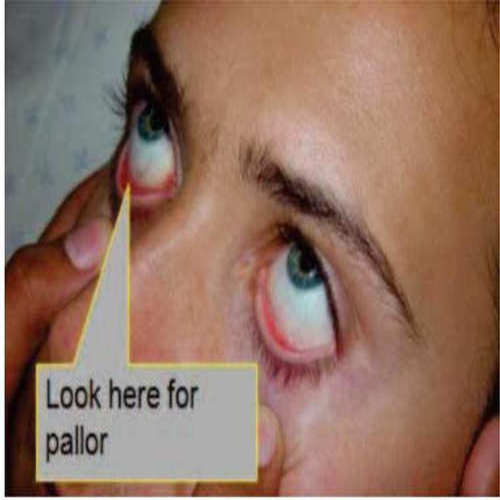
\includegraphics[width=\textwidth]{./clinicalPhysioPic/pallor1.jpg}
																	\subcaption{Site Of Examination of Pallor} 
																	\label{lpc}
																\end{subfigure}
																\hspace{\fill}
																\begin{subfigure}[t]{.23\textwidth}
																	\centering
																	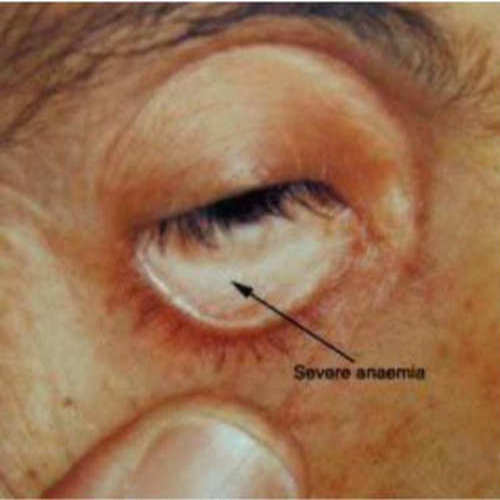
\includegraphics[width=\textwidth]{./clinicalPhysioPic/pallor2.jpg}
																	\caption{Lower Palpabral Conjunctiva In Severe Anemia}
																	\label{pallor}
																\end{subfigure}
																\hspace{\fill}
																\begin{subfigure}[t]{.23\textwidth}
																	\centering
																	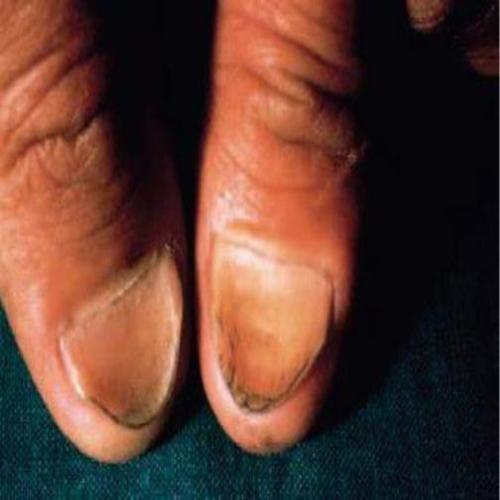
\includegraphics[width=\textwidth]{./clinicalPhysioPic/koilonychia.jpg}
																	\caption{Koilonychia}
																	\label{koilonychia}
																\end{subfigure}
																\hspace{\fill}
																\begin{subfigure}[t]{.23\textwidth}
																	\centering
																	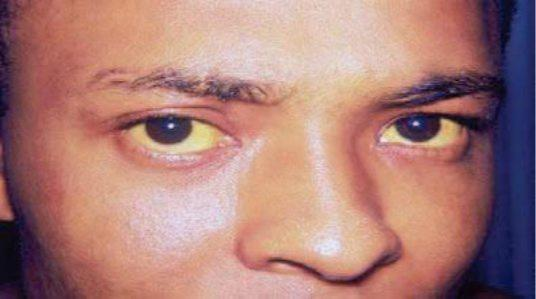
\includegraphics[width=\textwidth]{./clinicalPhysioPic/jaundice.jpg}
																	\caption{Icterus}
																	\label{icterus}
																\end{subfigure}
																\hspace{\fill}
																\begin{subfigure}[t]{.23\textwidth}
																	\centering
																	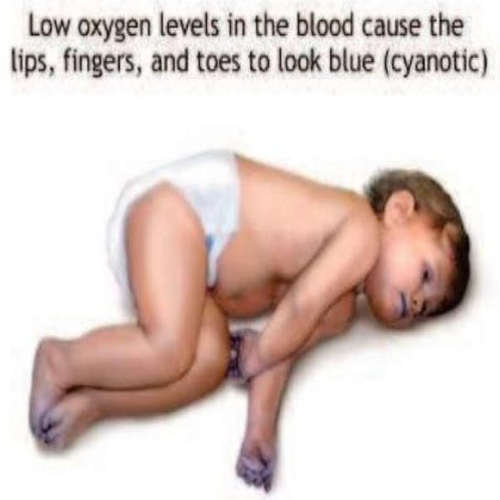
\includegraphics[width=\textwidth]{./clinicalPhysioPic/cyanosis4-0.jpg}
																	\caption{Cyanosis}
																	\label{cyanosis1}
																\end{subfigure}
																\hspace{\fill}
																\begin{subfigure}[t]{.23\textwidth}
																	\centering
																	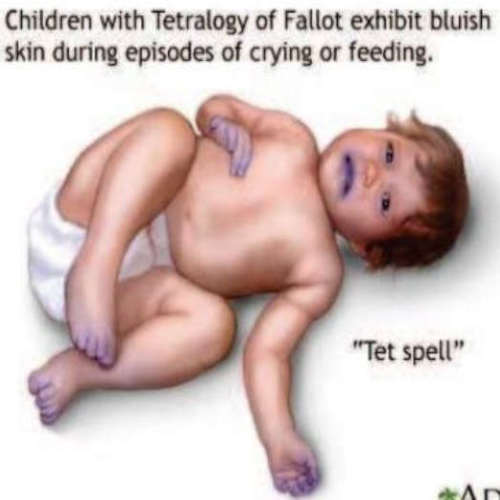
\includegraphics[width=\textwidth]{./clinicalPhysioPic/cyanosis4-1.jpg}
																	\caption{Cyanosis}
																	\label{cyanosis2}
																\end{subfigure}
																\hspace{\fill}
																\begin{subfigure}[t]{.23\textwidth}
																	\centering
																	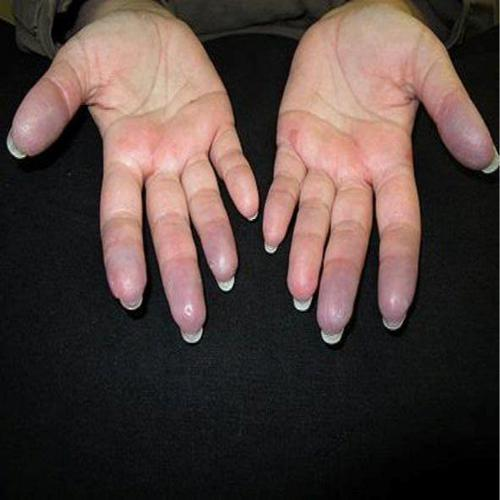
\includegraphics[width=\textwidth]{./clinicalPhysioPic/cyanosis4-2.jpg}
																	\caption{Cyanosis}
																	\label{Cyanosis3}
																\end{subfigure}
																\hspace{\fill}
																\begin{subfigure}[t]{.23\textwidth}
																	\centering
																	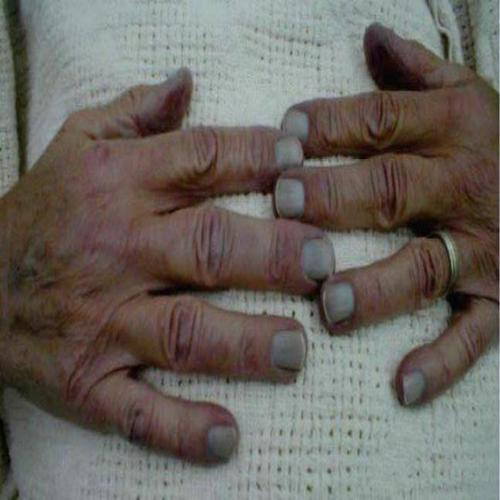
\includegraphics[width=\textwidth]{./clinicalPhysioPic/cyanosis4-3.jpg}
																	\caption{Cyanosis}
																	\label{Cyanosis4}
																\end{subfigure}
																\hspace{\fill}
																\begin{subfigure}[t]{.23\textwidth}
																	\centering
																	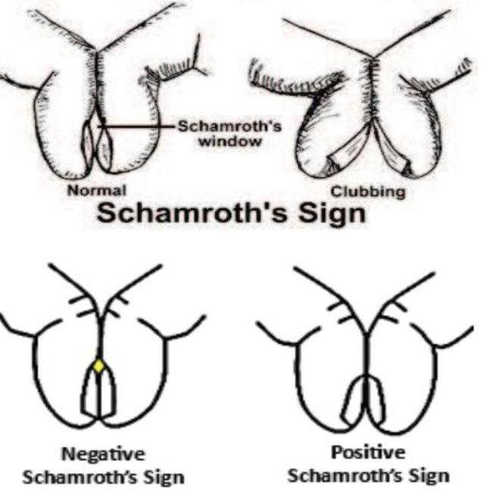
\includegraphics[width=\textwidth]{./clinicalPhysioPic/clubbing3-0.jpg}
																	\caption{Clubbing}
																	\label{Clubbing1}
																\end{subfigure}
																\hspace{\fill}
																\begin{subfigure}[t]{.23\textwidth}
																	\centering
																	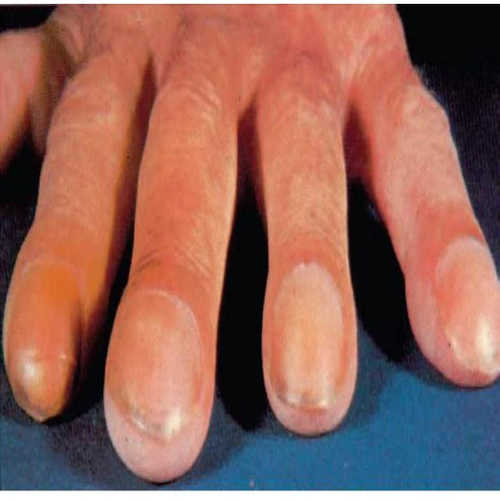
\includegraphics[width=\textwidth]{./clinicalPhysioPic/clubbing3-1.jpg}
																	\caption{Clubbing}
																	\label{Clubbing2}
																\end{subfigure}
																\hspace{\fill}
																\begin{subfigure}[t]{.23\textwidth}
																	\centering
																	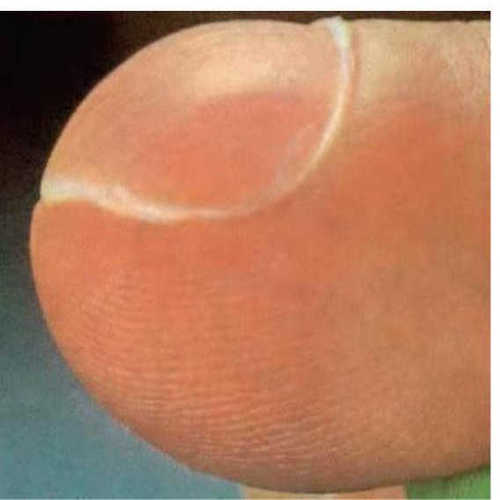
\includegraphics[width=\textwidth]{./clinicalPhysioPic/clubbing3-2.jpg}
																	\caption{Clubbing}
																	\label{Clubbing3}
																\end{subfigure}
																\hspace{\fill}
																\begin{subfigure}[t]{.23\textwidth}
																	\centering
																	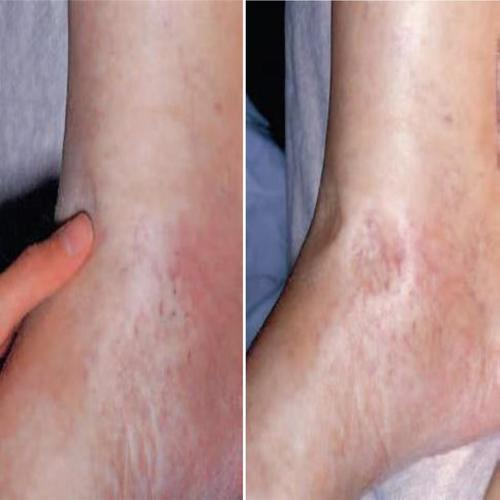
\includegraphics[width=\textwidth]{./clinicalPhysioPic/pittingPedalEdema.jpg}
																	\caption{Pedal Edema}
																	\label{PedalEdema}
																\end{subfigure}
																\caption*{General Examination}
															\end{figure}
															}
															The level of consciousness can be clear sensorium, drowsiness, stupor, semicoma and coma.
															\section*{Orientation To Time, Place And Person}
															Ask about the day, date, month, year and time of day. Subject should know where they are (e.g. home or hospital) Similarly test his orientation towards person.
															\section*{Body Build And Nourishment}
															Build refers to skeletal frame work and nourishment refers to muscular bulk. It should be observed whether he is well / moderately / thin built and nourished.
															\section*{Temperature}
															Recorded by a clinical thermometer.\newline
															\begin{itemize}
																\item{\textbf{Method of recording temperature:}}

																	Do not touch the bulb of the thermometer. Shake down the mercury column into the bulb. Keep it under the tongue with the mouth closed for one minute before reading the temperature.
																\item{\textbf{Sites of recording temperature:}}
																	\begin{itemize}%Sites of recording temperature:]
																		\setlength\itemsep{.5em}
																		\item{Mouth ( 36.6$^{\circ}$C to 37.2C$^{\circ}$C )}
																		\item{Axilla ( 0.5 $^{\circ}$C lower than oral temperature )}
																		\item{Rectum ( 0.5 $^{\circ}$C higher than oral temperature – Closer to core temperature )}
																	\end{itemize}
															\end{itemize}

															\section*{Pallor}
															Pallor of the skin and mucous membrane.
															\begin{itemize}
																\item{\textbf{Areas to look for pallor}}
																	\begin{itemize}
																		\item{Lower palpebral conjunctiva}
																		\item{Instruct the subject to look up and retract the lower lid to see the palpebral conjunctiva}
																		\item{Dorsum of tongue}
																		\item{Mucous membrane of oral cavity}
																		\item{Nail bed}
																		\item{Skin over palm and sole}
																	\end{itemize}

																\item{\textbf{Conditions where pallor is seen}}
																	\begin{itemize}
																		\item{Anemia – Reduced count of RBCs / Hb content in blood}
																		\item{Shock}
																	\end{itemize}
															\end{itemize}
															\section*{Jaundice ( Icterus )}
															Yellowish discoloration of the sclera, skin and the mucous membrane due to presence of excess bilirubin in blood of more than 2 $mg$\%
															\begin{itemize}
																\item{\textbf{Areas to look for jaundice}}
																	\begin{itemize}
																		\item{Bulbar conjunctiva of both eyes – Upper sclera}
																			(Instruct the subject to look down and retract the upper lid to view the sclera)
																		\item{Mucus membrane of oral cavity}
																			(especially the undersurface of tongue and floor of mouth)
																		\item{Nail bed}
																		\item{Skin}
																	\end{itemize}
																\item{\textbf{Causes of yellowish discoloration of skin}}
																	\begin{itemize}
																		\item{Jaundice, Carotenemia, Hemochromatosis}
																	\end{itemize}

																\item{\textbf{Hypercarotenemia occurs in}}
																	\begin{itemize}
																		\item{People who eat large quantity of raw carrots and tomatoes}
																		\item{Hypothyroidism.}
																	\end{itemize}
															\end{itemize}
															\section*{Cyanosis}
															It is the bluish discoloration of the skin and mucous membrane due to an increased quantity of reduced hemoglobin concentration of more than 5 gm in 100 ml of blood.
															\begin{itemize}
																\item{\textbf{Areas to look for cyanosis:}}
\begin{itemize}
\item{Lips}
\item{Tongue}
\item{Mucous membrane over the Palate}
\item{Conjunctiva}
\item{Tip of the nose and ear lobules}
\item{Extremities (fingers, toes and nail beds)}
																	\end{itemize}
																\item{\textbf{Types of Cyanosis:}}
\begin{itemize}
\item{	Central cyanosis}
\item{	Peripheral cyanosis}
\item{	Differential cyanosis}
\end{itemize}
\end{itemize}
\begin{table}[H]
	\centering
	\begin{tabular}{|p{.5in}|p{1in}|p{2.25in}|p{2.25in}|} 
		\hline
		\textbf{S.No.} & \textbf{Features}                                                 & \textbf{Central			Cyanosis}                                                      & \textbf{Peripheral			Cyanosis}                                           \\ 
		\hline
		1.							       & Mechanism                                                         & Right to left shunts or abnormal Hb or inadequate O$_2$ saturation             & Peripheral			stasis of blood                                             \\ 
		\hline
		2.							        & Site                                                              & Whole			body (Central parts of the body such as tongue plus peripherial			parts) & Nail			beds, nose tip, ear lobe, extremities (tips of fingers and toes)  \\ 
		\hline
		3.							       & Associated			with                                                 & Clubbing			and polycythemia							                                               & Not			associated with any other symptoms                                 \\ 
		\hline
		4.							        & Extremities                                                       & Warm                                                                             & Cold                                                                     \\ 
		\hline
		5.~							       & \begin{tabular}[c]{@{}l@{}}On			Warming\\Extremities\end{tabular} & No			change                                                                      & Disappears                                                               \\ 
			\hline
			6.							        & O2			Inhalation                                                   & Slight			improvement                                                             & No			change                                                              \\ 
			\hline
			7.							        & Arterial			PaO2							                                            & \textless{}85\%                                                                  & Normal                                                                   \\
			\hline
	\end{tabular}
\end{table}

\section*{Clubbing}
Bulbous enlargement of soft parts of the terminal phalanges with over curving of the nails both longitudinally and transversely.
\begin{itemize}
	\item{\textbf{Schamroth’s sign:}}
	\begin{itemize}
\item{When two fingers of both hands are held together with their nails facing each other, a diamond shaped space is seen. This space is lost in clubbing (Positive Schamroth’s sign).}
	\end{itemize}
\item{\textbf{Clubbing is seen in}}
	\begin{itemize}
\item{Bronchopulmonary diseases like bronchiectasis, lung abscess, empyema, chronic bronchitis and bronchogenic carcinoma}
\item{Cardiac diseases like congenital cyanotic heart disease and bacterial endocarditis}
\item{Gastro intestinal diseases like ulcerative colitis and liver cirrhosis}
\item{Endocrine disorders like acromegaly, thyrotoxicosis}
\item{Hereditary}
	\end{itemize}
\end{itemize}

\section*{Oedema}
It is the condition where there is accumulation of free fluid in the interstitial space. Pedal oedema is examined by pressing the skin and the tissue against the tibial bone just above the medial malleolus, sustaining the pressure for at least 15 seconds and releasing the pressure to look for pitting, if any. In bed ridden subjects oedema is examined by pressing over the presacral region.

\begin{itemize}
\item{\textbf{Types of oedema:}}
\begin{itemize}
\item{Pitting oedema – Heart failure, renal disease, hypoproteinemia}
\item{Non-pitting oedema – Myxoedema, filariasis}
\end{itemize}
\end{itemize}

\section*{Lymphadenopathy}
\begin{itemize}
	\item{\textbf{Group of nodes to be examined:}}
		\begin{itemize}
\item{Submental, submandibular, cervical, posterior auricular, occipital,  supraclavicular, axillary, inguinal and popliteal nodes.}
		\end{itemize}
\item{\textbf{Points to be noted while examining lymph nodes:}}
	\begin{itemize}
\item{Site, size, number, consistency (soft, firm or hard), tenderness, mobility, matted or discrete, fixity to skin, generalized or localized.}
	\end{itemize}
\item{\textbf{Examination of lymph nodes:}}
	\begin{itemize}
\item{Examiner should stand behind the sitting subject- Submental, submandibular, deep cervical nodes in the anterior triangle of neck}
\item{Examiner should stand in front of the sitting subject – deep cervical nodes in the posterior triangle of neck, posterior auricular and occipital nodes}
\item{Axillary nodes – sitting posture with abducted arm}
\item{Inguinal nodes – supine position with thigh flexed to 10$^{\circ}$}
\item{Popliteal nodes – Flex the knees and palpate deep into popliteal fossa}
	\end{itemize}
\end{itemize}

\section*{Questions}
\begin{enumerate}
\item{Where will you look for pallor?}
\item{What is cyanosis?}
\item{What are the types of Jaundice?}
\item{How do you detect clubbing?}
\item{What are the types of oedema and what are their causes?}
\item{What are the vital signs?}
\end{enumerate}

\newpage

\section*{\centering Case Sheet - General Examination Of The Subject}
															\begin{tabular}{p{5in} p{1.5in}}
																\textbf{Name:}  & \textbf{Age:}\\
																\textbf{Sex:}   & \textbf{Occupation:}
															\end{tabular}
															\begin{itemize}
\item[]Consciousness and orientation
\item[]Build and nourishment
\item[]Afebrile / Febrile
\item[]Pallor
\item[]Jaundice
\item[]Cyanosis
\item[]Clubbing 
\item[]Pedal edema
\item[]Lymphadenopathy
\item[]Vital Signs:
	\begin{itemize}
\item[]	Temperature
\item[]	Pulse rate
\item[]	Respiratory rate
\item[]	Blood pressure
	\end{itemize}
															\end{itemize}
\textbf{Inference:}
%------------------General Examination---}}}
%--------------Examination of Respiratory System--{{{

															\chapter*{\centering Examination Of Respiratory System}
\addcontentsline{toc}{chapter}{Examination Of Respiratory System}

															\begin{tabular}{p{5in} p{1in}}
																\textbf{Exp No:}  & \textbf{Date:}\\
															\end{tabular}
															\section*{Introduction}
															\addfig{%
																\begin{figure}
																	\centering
																	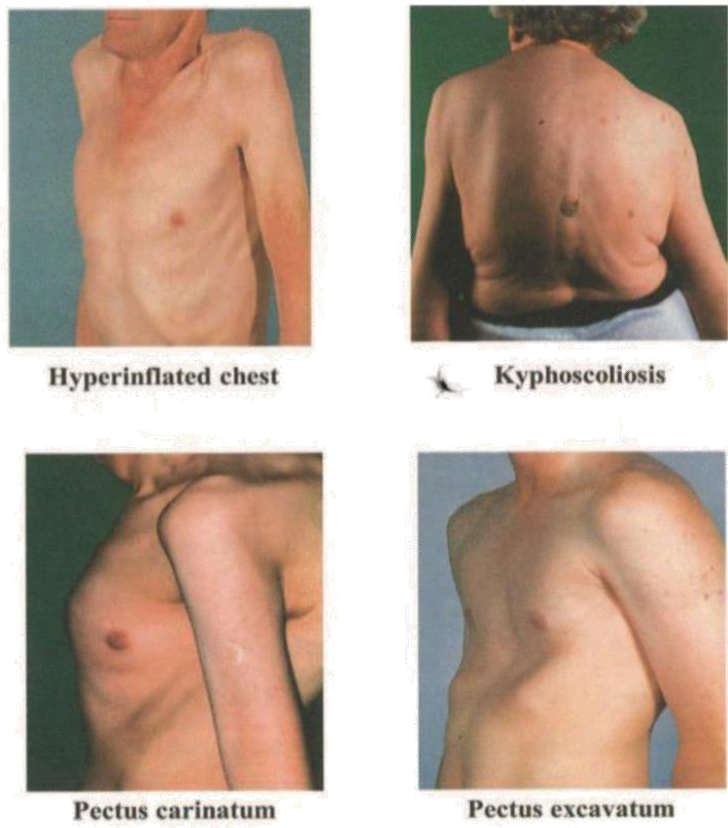
\includegraphics[scale=.5]{./clinicalPhysioPic/AbnormalChestShapes.jpg}
																	\caption*{Abnormal Chest Shapes}
																	\label{AbnormalChestShapes}
																\end{figure}
																}


															\paragraph{Important Anatomical Landmarks:}
															\begin{itemize}
\item{Midclavicular line – a vertical line that extends downwards from the midpoint between the middle of the suprasternal notch and the tip of the acromion.}
\item{Anterior axillary line – a vertical line extending downwards from the anterior axillary fold.}
\item{Posterior axillary line – a vertical line extending downwards from the posterior axillary fold.}
\item{Midaxillary line – a vertical line originating at a point midway between the anterior and posterior axillary line.}
															\end{itemize}
															\par
Examination of the respiratory system consists of Inspection, Palpation, Percussion \& Auscultation.

\section*{Inspection}
Ask the subject to sit on a stool with the chest and upper abdomen fully exposed.
\begin{enumerate}
\item{\textbf{Shape and symmetry of the chest}}
	\begin{itemize}
\item{Examine both the front and back of the chest.}
\item{Look for any skeletal deformities and drooping of shoulder.}
\item{Normal chest is bilaterally symmetrical and elliptical in cross section.}
\item{The transverse diameter is greater than the anteroposterior diameter with a ratio of 7:5  (Hutchinson’s index).}
\item[]\textbf{Abnormal Findings:}
	\begin{itemize}
\item{			Barrel shaped chest - anteroposterior diameter is more than the transverse diameter. It is seen in patients with severe COPD.}
\item{Pectus carinatum (pigeon chest) is a localized prominence of the sternum and adjacent costal cartilages. Occurs in rickets.}
\item{Pectus excavatum (funnel chest) is a developmental deformity with a localized depression of the lower end of sternum}
\item{Kyphosis is forward bending of the spine and Scoliosis is lateral bending. Kyphoscoliosis involves both deformities.}
	\end{itemize}
	\end{itemize}
\item{\textbf{Position of Trachea}}
	\begin{itemize}
\item{Stand in front of the subject. Ask the subject to look straight. Observe for any deviation of trachea. Normally, it is in the midline or slightly deviated to the right.}
\item{Look for any prominence of the sternocleidomastoid muscle. If it is prominent on one side, it indicates tracheal deviation to that side. This is TRIAL’S sign.}
	\end{itemize}
\item{\textbf{Apical impulse}\par Look for apical impulse over the precordium. ( Refer CVS Examination )}
\item{\textbf{Movement of the chest}\par The subject is instructed to take deep breaths. Observe, if the respiratory movements are equal on both sides.}
\item{\textbf{Respiratory Rate}\par Count the respiratory rate (breaths/min) for one minute, while you divert his attention by palpating the radial pulse. Normal rate ranges from 12-16 breaths / min. Increased rate of respiration is known as Tachypnoea and decreased rate is known as bradypnoea.}
\item{\textbf{Respiratory Movement}\par The subject is instructed to take deep breaths. Observe, if the respiratory movements are equal on both sides.}
	\begin{itemize}
		\item[]\textbf{Type of Respiratory movements:}\par Observe, if the respiration is predominantly thoracic or abdominal. During normal respiration, women use the intercostal muscles more than the diaphragm, and their respiratory movements are predominantly thoracic. Men rely more on the diaphragm and their respiratory movements are predominantly abdominal.
	\end{itemize}
\item{\textbf{Respiratory Rhythm}\par Observe, if the rhythm of respiration is regular or irregular.}
\item{\textbf{Abnormal pulsations, dilated veins, scars and sinuses over the chest wall:}}
\end{enumerate}

\section*{Palpation}
																\addfig{%
																	\centering
																	\begin{figure}
																	\begin{subfigure}[t]{\textwidth}
																		\centering
																		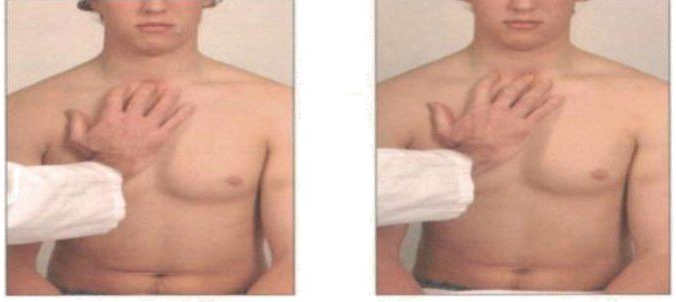
\includegraphics[scale=.5]{./clinicalPhysioPic/trachelShift.jpg}
																		\caption{Examination Of Tracheal Position}
																	\end{subfigure}
																	\hspace{\fill}
																	\begin{subfigure}[t]{\textwidth}
																		\centering
																		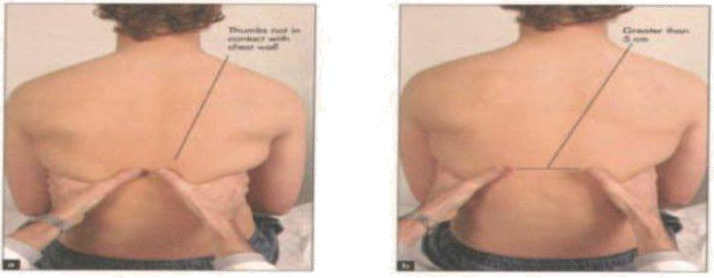
\includegraphics[scale=.5]{./clinicalPhysioPic/chestExpansion_LowerLobe.jpg}
																		\caption{Examination of chest expansion}
																	\end{subfigure}
																	\hspace{\fill}
																	\begin{subfigure}[t]{\textwidth}
																		\centering
																		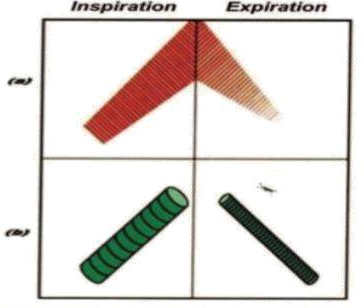
\includegraphics[scale=.5]{./clinicalPhysioPic/breathSounds.jpg}
																		\caption{Breath Sounds}
																	\end{subfigure}
																	\end{figure}
																	}
\begin{enumerate}
\item{Determine the position of mediastinum by examining the tracheal position and apical impulse.}
	\begin{itemize}
		\item[]\textbf{Tracheal Position:}
			\begin{itemize}
\item{Ask the subject to sit erect. Keep your index and ring finger of the right hand on medial ends of clavicle. Using the middle finger, gently feel for the trachea and assess whether it is in midline or deviated to one side.}
\item{Then, insinuate your middle finger into the space between the trachea and the sternocleidomastoid muscle on either side to assess the degree of yielding or resistance. }
\item{Common causes of Tracheal deviation}
\item{Towards the side of the lung lesion (pull) - Upper lobe collapse, Upper lobe fibrosis, Pneumonectomy}
\item{Away from the side of the lung lesion (push) - Tension pneumothorax, Massive pleural effusion}
			\end{itemize}
		\item[]\textbf{Apical impulse / Apex beat:}
			\begin{itemize}
\item{Palpate the precordium first with palm and then with ulnar border of hand to locate the apical impulse.}
\item{Place the index finger on the apical impulse and using the other hand, count the intercostal spaces with reference to sternal angle.}
\item{The normal apical impulse is felt at the left 5th intercostal space, half an inch medial to the left mid clavicular line.}
			\end{itemize}
		\item[]\textbf{Shift of mediastinum:} \par Shift of the upper mediastinum causes tracheal deviation. Displacement of apical impulse may indicate shift of lower mediastinum. Displacement of the cardiac impulse without tracheal deviation is usually due to left ventricular enlargement but can occur in scoliosis, kyphoscoliosis or severe pectus excavatum.
	\end{itemize}
\item{Respiratory Movements:}
	\begin{itemize}
\item{Assess expansion of the lower lobes by placing your hands firmly on the anterior chest wall. Extend your fingers around the sides of the subject’s chest. }
\item{Your thumbs should almost meet in the midline and hover just off the chest so that they can move freely with respiration.}
\item{Ask the subject to take deep breaths. Observe, whether your thumbs move equally on both sides.}
\item{To examine the movement of apical lobes, place the hands over the shoulders on both sides from behind. The degree of lift of the fingers indicates the degree of expansion of the apical lobes.}
\item{Examine the lower lobes of the lungs as explained before by placing the hands in the infrascapular area.}
\item{Reduced expansion on one side indicates abnormality on that side such as pleural effusion, lung collapse, pneumothorax and fibrosis}
	\end{itemize}
\item{Chest Expansion:}
	\begin{itemize}
\item{The chest expansion is measured quantitatively by using a measuring tape.}
\item{Hold the measuring tape around the chest wall just below the level of nipples.}
\item{The difference in expansion after a full expiration and a deep inspiration is the total chest expansion.}
\item{The normal expansion ranges from 5 to 8 $cm$.}
\item{It is decreased in restrictive lung diseases.}
	\end{itemize}
\item{Vocal fremitus / Tactile vocal fremitus:}
	\begin{itemize}
\item{	Ask the subject to repeat the word "ONE" or "NINETY NINE" in a clear voice.}
\item{Feel the vibrations using ulnar border of the hand in each intercostal space and compare it with the other side consecutively.}
\item{VF is increased in consolidation of lungs.}
\item{VF is decreased in pleural effusion and empyema.}
	\end{itemize}
\end{enumerate}


\section*{Percussion}
Percussion  allows  you  to  hear  the  pitch  and  loudness  of  the  percussed  note.  Percussion is done in sequence over corresponding areas on both sides of the chest.

\paragraph{Rules of percussion}
\begin{itemize}
\item{Place the middle finger of the left hand (Pleximeter finger) firmly against the chest,}
\item{aligned in the intercostal space.}
\item{Strike the centre of the middle phalanx of Pleximeter finger with the tip of your right middle finger (Percussing finger). Use a loose swinging movement of the wrist and not the forearm.}
\item{The long axis of the pleximeter finger should be parallel to the border of the organ being percussed.}
\item{Percussion is performed from a more resonant to less resonant area}
\end{itemize}

\paragraph{Methods of Percussion:}
\begin{itemize}
\item{Direct  percussion  -  Percuss  directly  over  the  medial  third  of  clavicles  without  an intervening finger.}
\item{Percuss the lung apices by placing the finger in the supraclavicular fossa.}
\item{Continue the percussion downwards on the anterior chest wall, axillae and posterior chest wall covering all the lung areas.}
\item{Always  compare  the  percussion  note  on  the  two  sides  of  the  chest systematically, moving from one side to the other side. Do not percuss all the way down one side and then down the other.}
\item{Normal lung produces a resonant note.}
\end{itemize}

\paragraph{Percussion Notes}
\begin{itemize}
\item{Resonant 		- 	Normal lung}
\item{Hyperresonant 	-	Pneumothorax}
\item{Dull 			-	Lung Consolidation, lung collapse, severe pulmonary 					fibrosis }
\item{Stony dull 		-	Pleural effusion}
\end{itemize}

\paragraph{Positioning Of Subject For Percussion:}
\textbf{To Percuss Lateral chest wall:}Ask the subject to keep the hands over the head.
\textbf{To Percuss Posterior chest wall:}Ask the subject to fold the arms across the front of the chest which will move the scapulae laterally.

\section*{Auscultation:}
\begin{itemize}
\item{The  stethoscope  is  used  to  auscultate  the  breath  sounds,  added  sounds  and  vocal resonance.}
\item{Instruct the subject to take deep breaths with open mouth.}
\item{With the diaphragm of the stethoscope, auscultate all areas of the lung.}
\item{As with percussion, listen to the sounds in comparable positions on either side alternately, switching back and forth from one side to the other side.}
\item{Normal breath sounds auscultated are known as Vesicular breath sounds. They are low pitched and have a rustling quality. There is no distinct pause between the end of inspiration and the beginning of expiration. Sound is heard throughout inspiration and only during one third of expiration.}
\item{Abnormal breath sounds are known as bronchial breath sounds.}
\end{itemize}

\paragraph{Bronchial Breath Sounds:}
\begin{itemize}
\item{It is a high-pitched breath sound with a hollow or blowing quality. The breath sounds are heard throughout inspiration and expiration. There is a distinct pause between the inspiration and expiration.}
\item{Bronchial breath sounds are heard in pulmonary consolidation (pneumonia) and in fibrosis.}
\end{itemize}

\paragraph{Causes for absence of breath sounds}
\begin{itemize}
	\item[]Pleural effusion, Pneumothorax.
\end{itemize}

\paragraph{Vocal Resonance:}
\begin{itemize}
\item{It is the auscultatory component of vocal fremitus.}
\item{Ask the subject to repeat ''ONE'' and auscultate in all the lung areas consecutively on both sides to assess the quality and amplitude of vocal resonance.}
\item{Vocal resonance is increased in consolidation and decreased in pleural effusion, pneumothorax and fibrosis.}
\end{itemize}

\paragraph{Adventitious or Added Sounds}
There are abnormal sounds that arise in the lung or in the pleura.
\begin{itemize}
\item{\textbf{Wheeze / Rhonchi:}\par Wheeze is a continuous musical sound, heard due to narrowing of airways. It is heard in bronchial asthma.}
\item{\textbf{Crackles/ Rales/ Crepitations:}\par Crackles are short, explosive sounds often described as bubbling sounds. Crackles may result from sudden opening of previously closed small airways. It may also be heard when air bubbles through secretions in major bronchi. It is heard in bronchiectasis and pulmonary edema.}
\item{\textbf{Pleural rub:}\par It is a creaking sound produced when inflamed parietal and visceral pleurae slide over one another. It is heard in pleuritis.}
\end{itemize}

\paragraph{Note:}
Examination of respiratory system is carried out in the following lung areas.
\begin{itemize}
\item{Supraclavicular}
\item{Infraclavicular}
\item{Mammary}
\item{Inframammary}
\item{Axillary}
\item{Infraaxillary}
\item{Suprascapular}
\item{Interscapular}
\item{Infrascapular}
\end{itemize}

\section*{Questions:}
\begin{enumerate}
\item{What is the normal Respiratory rate?}
\item{What is Tachypnoea?}
\item{What is dyspnoea?}
\item{Name the muscles of inspiration and expiration.}
\item{Name one condition in which vocal fremitus is increased and decreased.}
\item{What are the normal breath sounds?}
\item{What are Wheezes and Crackles?}
\end{enumerate}
%-------------------------}}}
%------------Respiratory Efficiency test---{{{

															\chapter*{\centering Respiratory Efficiency Test}
\addcontentsline{toc}{chapter}{Respiratory Efficiency Test}

															\begin{tabular}{p{5in} p{1in}}
																\textbf{Exp No:}  & \textbf{Date:}\\
															\end{tabular}
															\section*{Aim}
															To assess the efficiency of the respiratory muscles.
															\section*{Apparatus}
															Inch tape, BP apparatus, Peak flow meter, Match stick, Candle and Stop watch .
															\section*{Tests:}
															\begin{enumerate}
																\item{Breath holding time (BHT):\par Ask the subject to sit quietly for a few minutes breathing normally. Ask the subject to pinch his nostrils with the thumb and index finger and to hold the breath after a normal inspiration and start the stop watch. The time duration for which the subject is able to hold the breath is noted. Make three such observations at an interval of five minutes. Similarly, record the breath holding times after quiet expiration, deep inspiration and deep expiration.i%
																	epackage{multirow}
																	
																	\begin{table}[H]
																		\centering
\begin{tabular}{|l|l|l|l|l|} 
																			\hline
																			\multirow{2}{*}{\begin{tabular}[c]{@{}l@{}}\\Breathholding at the end of \end{tabular}} & \multicolumn{3}{l|}{Time(sec)} & \multirow{2}{*}{BestValue}  \\ 
																				\cline{2-4}
																				                                                                                        & 1 & 2 & 3                      &                             \\ 
																															\hline
																															QuietInspiration                                                                        &   &   &                        &                             \\ 
																															\hline
																															QuietExpiration                                                                         &   &   &                        &                             \\ 
																															\hline
																															DeepInspiration                                                                         &   &   &                        &                             \\ 
																															\hline
																															DeepExpiration                                                                          &   &   &                        &                             \\
																															\hline
																		\end{tabular}
																	\end{table}
																		}
																\item{Expiratory blast test:\par BP apparatus is required for this test. The rubber tube leading from the mercury reservoir to the cuff is disconnected. Ask the subject to take a deep inspiration and blow into the tube to raise the mercury column to the highest level possible. A normal subject can raise the mercury column to 65-100 mmHg or more during a single forceful expiration.}
																\item{Snider’s test:\par A normal adult should be able to blow out a burning match stick or candle held at a distance of 30 cms in front of his face, with a single forceful expiration}
																\item{Respiratory endurance test: \par Ask the subject to take a deep breath, close his nostrils and blow into the rubber tubing to raise the mercury column to 40 mmHg level in the manometer. He is instructed to maintain the mercury level at 40mmHg as long as possible. Normal person can hold it at the same level for 40-70 seconds or more.}
																\item{Peak expiratory flow rate: \par Wright’s Peak flow meter measures the maximum flow rate which is achieved during a single forced expiration. It does not measure the volume of air exhaled.\newline
																	\paragraph{Procedure}
																	Ask the subject to take a deep breath and then to blow hard into the mouth piece of the flow meter forcefully with his nostrils closed. The reading on the dial is the PEFR in litres/min. Repeat the procedure thrice at an interval of 1-2 minutes. Normal range is 300-500 litres/minute.}
															\end{enumerate}
\section*{Questions:}
\begin{enumerate}
\item{ What is the normal breath holding time?}
\item{ What is expiratory blast test?}
\item{ Define PEFR? What is the normal value?}
\item{ What are the uses of Wright’s peak flow meter in clinical practice?}
\end{enumerate}
%----------------------------}}}
%----------------Spirometery---------------{{{

															\chapter*{\centering Spirometry}
\addcontentsline{toc}{chapter}{Spirometry}

															\begin{tabular}{p{5in} p{1in}}
																\textbf{Exp No:}  & \textbf{Date:}\\
															\end{tabular}
															\section*{Aim:}
\addfig{%
	\begin{figure}[H]
		\begin{subfigure}{\textwidth}
			\centering
			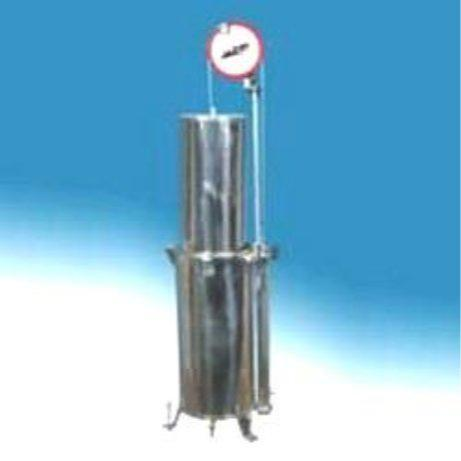
\includegraphics[scale=.5]{./clinicalPhysioPic/spirometry.jpg}
			\caption{Spirometer}
			\label{Spirometer}
		\end{subfigure}
		\hspace{\fill}
		\vspace{1cm}
		\begin{subfigure}{\textwidth}
			\centering
			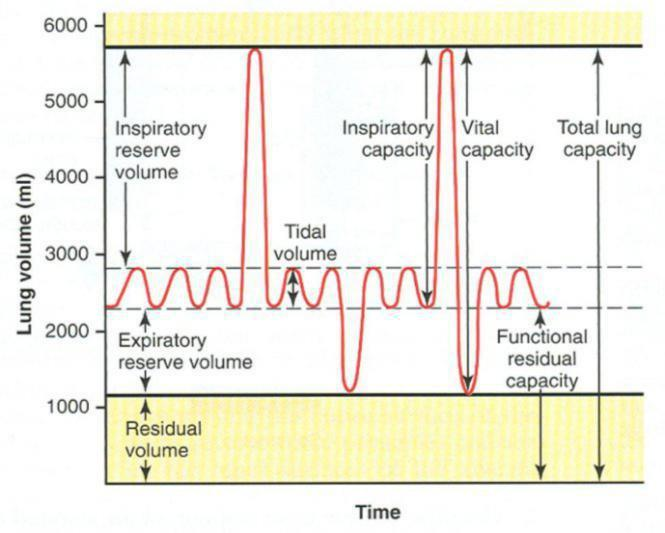
\includegraphics[scale=.5]{./clinicalPhysioPic/spirogram.jpg}
			\caption{Lung Volumes \& Capacities}
			\label{lungVolumes}
		\end{subfigure}
	\end{figure}
	}
															To measure Tidal Volume, Expiratory Reserve Volume and Vital Capacity in the given subject.
															\section*{Apparatus Required:}
															Student’s Spirometer
															\section*{Spirometer :}
															Student’s Spirometer is also known as Vitalograph or Simple Spirometer. It consists of a double-walled metal cylinder. The outer container is filled with water in which a light-metal gas bell of 6 litre capacity floats. The water acts as an air-tight seal. The bell is attached to a counter-weight by a chain passing over a graduated frictionless pulley. The pulley bears a spring-mounted indicator needle that moves with the pulley and indicates the volume of air present in the bell. A corrugated rubber tube with a mouthpiece acts as the inlet tube.
															\section*{Procedure}
															All the procedures should be done in standing posture.
															\begin{enumerate}
																\item{															\textbf{Tidal Volume:}	The volume of air inspired or expired during quiet respiration}
																	\begin{itemize}
\item{															Set the pointer at zero}
\item{															Ask the subject to take a few normal breaths with nostrils closed}
\item{															Ask the subject to breathe out into the mouth piece at the end of normal inspiration}
\item{															Record the reading as Tidal Volume}
																	\end{itemize}
																\item{															\textbf{Expiratory Reserve Volume:} The volume of air that can be expired forcefully after a normal expiration}
																	\begin{itemize}
\item{															Set the pointer at zero}
\item{															Ask the subject to take a few normal breaths with nostrils closed}
\item{															At the end of normal expiration ask the subject to breathe out forcefully into the mouthpiece to the maximum}
\item{															Record the reading as Expiratory Reserve Volume}
																	\end{itemize}
																\item{															\textbf{Vital Capacity :} The maximum volume of air that can be forcibly expired after maximum inspiration}
																\begin{itemize}
\item{															Set the pointer at zero}
\item{															Ask the subject to take a few normal breaths with nostrils closed}
\item{															Ask the subject to inspire to the maximum and then to expire forcefully and completely into the mouthpiece}
\item{															Record the reading as Vital Capacity}
															\end{itemize}
															\end{enumerate}

															\section*{Result}
														\begin{itemize}
														\item[]	Tidal Volume						=\rule{5cm}{1mm}	
\item[]		Expiratory Reserve Volume				=\rule{5cm}{1mm}
\item[]			Vital Capacity						=\rule{5cm}{1mm}	
														\end{itemize}

														\section*{Observations}

															\begin{tabular}{p{5in} p{1in}}
																\textbf{Name:}  & \textbf{Age:}\\
																\textbf{Sex:}   & \textbf{Occupation:}
															\end{tabular}

\begin{table}[H]
\centering
\begin{tabular}{|l|l|l|l|} 
	\hline
	\textbf{Lung			Volumes \& Capacities}~							 &  \textbf{Reading			1} &  2\textbf{Reading			2} &  \textbf{Reading			3}  \\ 
	\hline
	TidalVolume                                   &                       &                        &                        \\ 
	\hline
	ExpiratoryReserve Volume                      &                       &                        &                        \\ 
	\hline
	VitalCapacity                                 &                       &                        &                        \\
	\hline
\end{tabular}
\end{table}
														\section*{Questions :}
														\begin{enumerate}
\item{														 What are the factors affecting Vital Capacity ?}
\item{														 Name the volumes and capacities that cannot be measured directly using Student’s Spirometer.}
\item{														 What is Breathing Reserve ?}
\item{														 What is Dyspnoeic Index ?}
\item{														 Give the normal values of Tidal Volume, Vital Capacity \& Expiratory Reserve Volume in adult men and women.}
\item{														 Comment on FVC and FEV1 \% in Restrictive and Obstructive lung disorders.}
														 Define Dead space. Write a note on Anatomical and Physiological Dead space.

														\end{enumerate}
														%---------}}}
%---------Stethography----{{{
															\chapter*{\centering Stethography}
\addcontentsline{toc}{chapter}{Stethography}
															\begin{tabular}{p{5in} p{1in}}
																\textbf{Exp No:}  & \textbf{Date:}\\
															\end{tabular}
\section*{Aim:}
\addfig{%
	\centering
	\begin{figure}[H]
		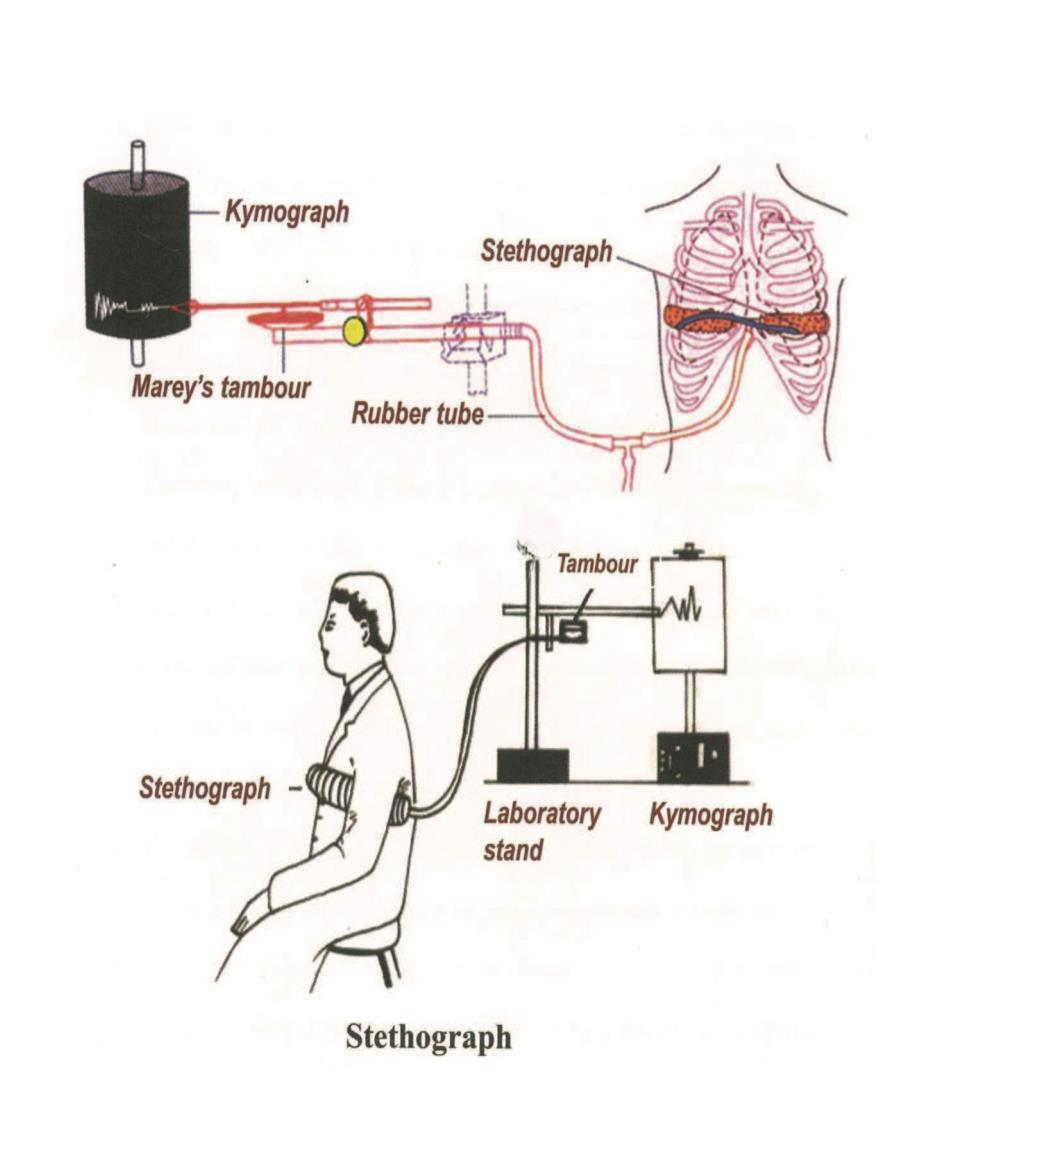
\includegraphics[scale=.4]{./clinicalPhysioPic/stethography.jpg}
		\caption*{Stethography}
		\label{stethography}
	\end{figure}
	}
To record Respiratory movements using Stethograph in the given subject.
\section*{Apparatus Required:}
Stethograph , Marey’s tambour, Kymograph, Stop watch, A glass of drinking water .
Stethograph consists of a corrugated rubber tube with one end sealed and the other end connected to Marey’s tambour. Marey’s tambour has a small metal cup with a rubber diaphragm. When the Stethograph is connected to the tambour, the pressure change in the Stethograph is transmitted to it. Pressure changes are recorded on a moving drum using a lever placed on the rubber diaphragm. During chest expansion, the volume of the stethograph increases and pressure decreases. This causes downward movement of the rubber diaphragm on the Marey’s tambour. The lever on the Marey’s tambour moves down. So inspiration is recorded as a downstroke.
\section*{Procedure :}
\begin{itemize}
\item{Ask the subject to sit with his back towards the recording setup}
\item{Tie the Stethograph at mid-chest level ( 4th intercostals space )}
\item{Connect the Stethograph to the Marey’s tambour. Bring the writing lever in contact with the smoked drum}
\item{Check for the movement of lever with movement of chest wall}
\end{itemize}
\subsection*{Normal Respiration :}
\begin{itemize}
\item{Record few normal respiratory movements}
\item{Upstroke of pointer corresponds to expiration and down stroke to Inspiration}
\end{itemize}
\subsection*{Effect of Hyperventilation :}
\begin{itemize}
\item{Record few normal respiratory movements}
\item{Ask the subject to hyperventilate for 2 minutes}
\item{Record the findings}
\item{Hyperventilation is followed by a short period of Apnoea. Apnoea is recorded as a straight line on the drum.}
\end{itemize}
\subsection*{Effect of Swallowing :}
\begin{itemize}
\item{Record few normal respiratory movements.}
\item{Instruct the subject to drink from a glass of water continuously and record the effects.}
\item{Respiration stops during swallowing. It is recorded as a straight line. This is known as Deglutition Apnoea.}
\end{itemize}

\subsection*{Breath Holding time :}
\begin{itemize}
\item{Record few normal respiratory movements.}
\item{Instruct the subject to hold his breath for as long as possible at the end of normal Inspiration and record the Breath holding time. It is recorded as a straight line. This period is followed by respiratory excursions. This is called Breaking point.}
\item{Repeat the procedure at the end of Normal expiration, Maximum Inspiration and Maximum expiration and record the Breath holding time for each.}
\end{itemize}

\subsection*{Effect of Exercise :}
\begin{itemize}
\item{Record few normal respiratory movements.}
\item{Detach the tube and ask the subject to exercise for 3 minutes (sit ups).}
\item{Re-attach the tube and record the respiratory movements.}
\item{Hyperpnoea –i.e. increased rate and depth of respiration is seen. Slowly the respiration returns back to normal.}
\end{itemize}

\section*{Questions :}
\begin{enumerate}
\item{What is Deglutition Apnoea ?}
\item{What is the effect of Exercise on respiration ?}
\item{What is the normal Breath-holding time in adults?}
\item{What is the physiological basis for Breaking point ?}
\item{Mention the changes in respiration following hyperventilation.}
\item{What is Periodic breathing ? Give few examples.}
\end{enumerate}
%--------}}}
%--------------------Examination of Arterial Pulse------{{{

															\chapter*{\centering Examination of the Arterial Pulse}
\addcontentsline{toc}{chapter}{Examination of the Arterial Pulse}
															\begin{tabular}{p{5in} p{1in}}
																\textbf{Exp No:}  & \textbf{Date:}\\
															\end{tabular}
\section*{Definition:}
\addfig{%
	\centering
	\begin{figure}[H]
		\begin{subfigure}[t]{.29\textwidth}
			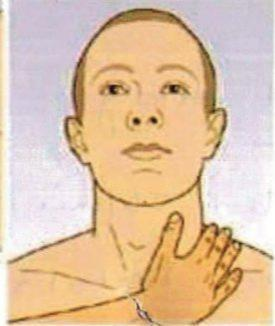
\includegraphics[height = 5cm, width = 5cm]{./clinicalPhysioPic/carotidPulse.jpg}
			\subcaption{Examination Of Carotid Pulse}
			\label{carotidPulse}
		\end{subfigure}
		\hspace{\fill}
		\begin{subfigure}[t]{.29\textwidth}
			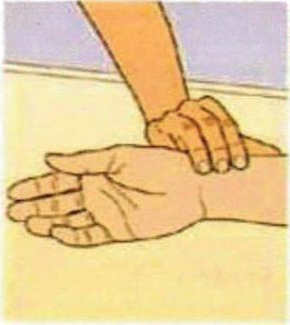
\includegraphics[height = 5cm, width = 5cm]{./clinicalPhysioPic/radialPulse_1.jpg}
			\subcaption{Examination Of Radial Pulse}
		\end{subfigure}
		\hspace{\fill}
		\begin{subfigure}[t]{.29\textwidth}
			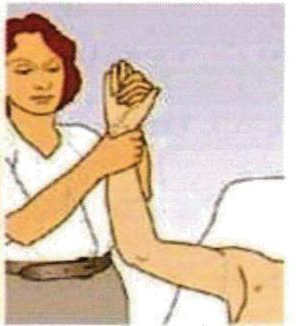
\includegraphics[height= 5cm, width = 5cm]{./clinicalPhysioPic/collapsingPulse.jpg}
			\subcaption{Examination Of Collapsing Pulse}
			\label{collapsingPulse}
		\end{subfigure}
		\begin{subfigure}[t]{.29\textwidth}
			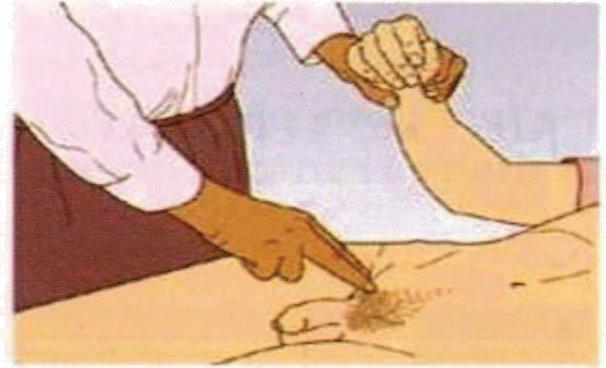
\includegraphics[height=5cm, width=5cm]{./clinicalPhysioPic/radioFemoralDelay.jpg}
			\subcaption{Examination Of Radio Femoral Delay}
			\label{radioFemoralDelay}
		\end{subfigure}
		\hspace{\fill}
		\begin{subfigure}[t]{.29\textwidth}
			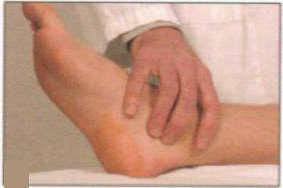
\includegraphics[height=5cm, width=5cm]{./clinicalPhysioPic/posteriorTibial.jpg}
			\subcaption{Examination Of Posterior Tibial Artery}
			\label{posteriorTibial}
		\end{subfigure}
		\hspace{\fill}
		\begin{subfigure}[t]{.29\textwidth}
			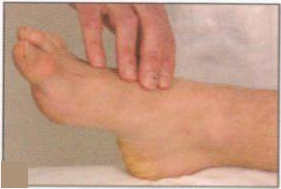
\includegraphics[height=5cm,width=5cm]{./clinicalPhysioPic/dorsalisPedis.jpg}
			\subcaption{Examination Of Dorsalis Pedis Artery}
			\label{dorsalisPedis}
		\end{subfigure}
		
		\caption*{Examination Of Arterial Pulses}
		\label{arterialPulses}
	\end{figure}
	}
Arterial pulse is the rhythmic expansion of the arterial wall due to transmission of pressure waves along their walls during each systole of the heart.

\section*{Procedure:}
Examination of the arterial pulse is done to assess the following parameters:
\begin{enumerate}
	\item{\textbf{Rate:}\newline
		Normal rate is 60-100 /min.
		\par \textbf{Bradycardia :} When the pulse rate is less than 60/min
		\begin{itemize}
			\item[]\textbf{Physiological causes:} Sleep, old age, trained athletes
			\item[]\textbf{Pathological causes:} Heart blocks, Myxoedema, increased intracranial tension
		\end{itemize}
		\par \textbf{Tachycardia:}When the pulse rate is more than 100/min .
		\begin{itemize}
			\item[]\textbf{Physiological causes:}Exercise, Emotion, Excitement and in newborn
			\item[]\textbf{Pathological causes:}Fever ,anemia, Thyrotoxicosis.
		\end{itemize}
		}

	\item{\textbf{Rhythm}
When the interval between the pulse wave is constant, the pulse is said to be regular in rhythm .When the spacing is not constant the pulse is irregular.	
		\par \textbf{Sinus arrhythmia:} This is a normal finding .The pulse rate increases during inspiration and decreases during expiration. 		
		\par \textbf{Abnormal Rhythms (Arrythymias):}
		\begin{itemize}
			\item[]				\textbf{Regularly irregular rhythm:} Extrasystoles or ventricular premature contractions
			\item[]				\textbf{Irregularly irregular rhythm:} Atrial Fibrillation.
		\end{itemize}
		}
	\item{\textbf{Volume}
\par It is the degree of expansion of arterial vessel wall during the passage of the pulse wavefront.
		\begin{itemize}
\item{The pulse volume depends on the stroke volume and arterial compliance .}
\item{High volume pulse or pulsus magnus is observed in aortic incompetence, beriberi, anemia and fever.}
\item{Low volume pulse or pulsus parvus is observed in aortic stenosis and shock.}
		\end{itemize}
		}

	\item{\textbf{Character}
\par Character of the pulse wave is best appreciated by palpating the carotid    artery in the neck.
		\paragraph{Certain Abnormal character of pulse:}
		\begin{itemize}
			\item[]\textbf{Collapsing pulse:} Also known as water hammer pulse, is characterized by rapid upstroke and rapid downstroke. It is observed in aortic regurgitation.
			\item[]\textbf{Pulsus alternans:} A pulse waveform showing alternating strong and weak beats .It is observed in left ventricular failure.
		\end{itemize}
		}
	\item{\textbf{Condition of the vessel wall}
\par It is assessed in the radial artery .The artery in the young individual is elastic and compliant .It becomes thickened like a cord due to atherosclerosis and calcification in old age. Hence it becomes palpable in them.
		}
	\item{\textbf{Radiofemoral delay}
\par Both radial and femoral artery are palpated simultaneously by the examiner .Normally, there is no delay between the appearance of pulse in the radial and femoral artery.
		\par Radiofemoral delay is seen in Coarctation of Aorta, where radial pulse is felt before femoral pulse.}
\end{enumerate}

\section*{Examination of other peripheral pulses.}
\addfig{%
	\centering
	\begin{figure}[H]
		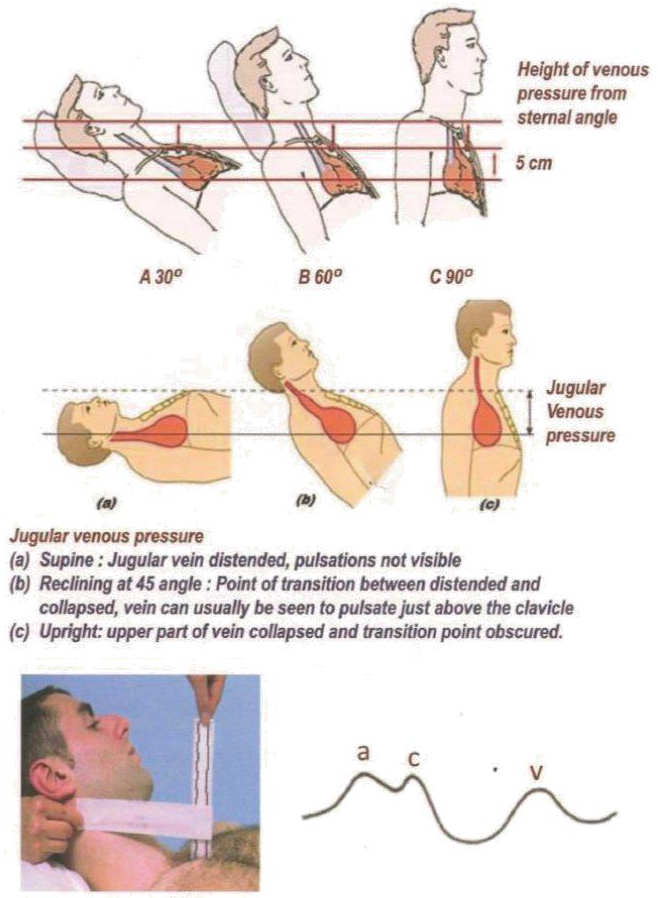
\includegraphics[width = 15cm, height = 15cm]{./clinicalPhysioPic/jvp.jpg}
		\caption*{Examination Of Jugular Venous Pulse \& Measurement of Jugular Venous Pressure}
		\label{jvp}
	\end{figure}
	}


\par
\subsection*{\textbf{Radial pulse :}} Palpated against the radial styloid process.  Radial pulse is examined for Rate, Rhythm and Volume Hold the subjects right arm in the semi prone position with slight flexion at the wrist. The radial pulse is palpated using the right index, middle and ring fingers by gently compressing the artery against the radial styloid process. Count for one full minute.
\subsection*{\textbf{Brachial pulse:}} Palpated in the antecubital fossa medial to the biceps tendon.
\subsection*{\textbf{Carotid pulse:}} Palpated between the thyroid cartilage and anterior border of the sternocleidomastoid muscle .Do not examine the carotid pulse simultaneously on both sides.
\subsection*{\textbf{Popliteal pulse :}}The subject’s knees are flexed at an angle of 120$^{\circ}$ .The artery is palpated with the finger tips of both the hands placed in the popliteal fossa with the thumb resting on his patella.
Posterior tibial pulse: Palpated 1cm below and behind the medial malleolus .
\subsection*{\textbf{Dorsalis pedis pulse:}} Palpated just lateral to the extensor hallucis tendon .

\section*{Examination Of The Venous Pulse :}
Measurement of venous waves in the neck helps to determine the right atrial hich is transmitted to the right internal jugular vein .
\begin{itemize}
\item{Ask the subject to lie down in a couch ,and raise the head end of the couch to 45$^{\circ}$, so that the back of the subject is supported and the neck muscles are relaxed.}
\item{Ask the subject to turn to the left and look for venous pulsations in between the two heads of sernocleidomastoid on the right side of his neck.}
\item{In normal persons in this position, the venous pulse appears just at the upper border of the clavicle.}
\item{Venous pulse above the clavicle in this position is considered as raised JVP.}
\end{itemize}
\subsection*{Measurement}
\begin{itemize}
\item{Place a scale at the level of the top of the pulse wave in the neck horizontally Measure the vertical distance from sternal angle to the horizontal scale, by using another scale.}
\item{Pulsation in the internal jugular vein is more reliable as it directly reflects the pressure changes in the right atrium .}
\end{itemize}

\subsection*{External jugular veins are not reliable because:-}
\begin{itemize}
	\item[]{External jugular veins has many valves.}
	\item[]{External jugular vein passes through fascial planes, in the neck. }
\end{itemize}
\subsection*{The venous pulse can be differentiated from arterial pulse in the neck by}
\begin{itemize}
\item[]{Venous pulse is better seen than felt .Arterial pulse is better felt.}
\item[]{Venous pulse has a definite upper level, which falls during inspiration.}
\item[]{Gentle pressure on the right hypochondrium will raise the venous pulse level due to a transient increase in venous return (Hepato jugular reflex).}
\item[]{By exerting moderate pressure above the clavicle with a finger, venous pulse can be obliterated.}
\item[]{Two to three waves can be seen in venous pulse.}
\end{itemize}

\section*{Questions:}
\begin{enumerate}
\item{Define pulse.}
\item{What is the cause for sinus bradycardia in athelets?}
\item{How will you examine for collapsing pulse? Name a condition producing collapsing pulse?}
\item{What is pulse deficit?}
\item{What is pulsus alternans?}
\item{What is pulsus paradoxus?}
\item{What are the waves seen in JVP?}
\end{enumerate}
%-------------------------------------------------------------}}}
%--------Examination of CVS----{{{
															\chapter*{\centering Examination Of Cardiovascular System}
\addcontentsline{toc}{chapter}{Examination Of Cardiovascular System}
															\begin{tabular}{p{5in} p{1in}}
																\textbf{Exp No:}  & \textbf{Date:}\\
															\end{tabular}
The cardiovascular system is examined to assess the functions of the heart and blood vessels as follows:
\begin{enumerate}
\item{General Examination}
\item{Examination of Arterial Pulse}
\item{Examination of the Jugular Venous Pulse / Pressure}
\item{Examination of Blood Pressure}
\item{Examination of Precordium}
\end{enumerate}

(\emph{Refer the respective experiments for General Examination, Examination of Arterial Pulse, Examination of Jugular Venous Pulse and Blood Pressure})

\section*{Examination Of Precordium}
\par
Precordium is the anterior aspect of the chest wall overlying the heart. Examination of precordium is done under the following headings.
\subsection*{Inspection:}
\par
\begin{itemize}
\item{Examine the subject in sitting posture in good day light , stripped to the waist so as to expose the precordium fully.}
\item{Shape and Symmetry of the chest wall}
\item{Tracheal position}
\item{Apical Impulse}
\item{Abnormal pulsations over the precordium}
\item{Skeletal deformities - Abnormal bulge/ depression over the precordium}
\item{Dilated veins over the precordium}
\item{	Look for the apical impulse in relation to the left nipple. Apical impulse is usually seen just below and medial to the nipple.}
\item{	Look for pulsation in the other areas of the precordium, specially pulmonary, aortic and left parasternal area.}
\item{	Inspect for any bulge in the precordium and any dilated and engorged superficial veins in the precordium. Precordial bulge is seen in congenital heart disease. Engorged veins indicate superior or inferior venacaval obstruction.}
\end{itemize}

\subsection*{Palpation}

\emph{( Refer Respiratory system for inspection and palpation of Tracheal position)}
\begin{itemize}
\item{Confirm the tracheal position}
\item{Confirm the apical impulse}
\item{Palpate for any thrill}
\item{Palpate for parasternal heave}
\item{Palpate for any abnormal pulsations}
\item{\textbf{Apical Impulse / Apex beat:}
	\par
	Apical impulse is defined as the lowermost and outermost definite cardiac Impulse. It is normally located in the left fifth intercostal space half an inch medial to mid clavicular line.
	\par
	First, place the palm on the precordium to feel the apical impulse and the n place the ulnar border of the palm horizontally in the intercoastal space where the pulsation is felt. Finally the apex beat is localised by the tip of the index finger C count the intercostal spaces with reference to the sterna angle (Angle of Lewis) – the most prominent point on the sternum. The second rib joins the manubrium sternum. The space below the second rib is the second intercostal space and accordingly other intercostals spaces are counted. 
	\par
	Note the position of the apex in the intercostals space with relation of midclavicular line.
	\par
	If the apex beat is not palpable in the supine posture, ask the subject to sit and lean forward. If apex beat is still not palpable, palpate the corresponding area of the chest on the right side. Despite all efforts apex beat may still not be palpable for following reasons.
	\begin{itemize}
\item{ Located behind a rib}
\item{ Chest wall may be thick due to fat or muscle.}
\item{ Emphysematous lung may cover part of the heart.}
\item{ In females, the breast may be pendulous.}
	\end{itemize}
	\par
	Normally the apical impulse just touches and lifts the examining finger. The abnormal characters are : Tapping , Hyperdynamic and Heaving apical impulse.
	}
\item{\textbf{Thrill}:
	\par
	Palpate all over the precordium for thrill with the palm of the hand. A palpable murmur is called as thrill which is due to vibrations from heart or the great vessels. It is due to abnormal flow through a normal valve or a normal flow through an abnormal valve. Thrill is felt as a feeling similar to the purring of the cat.
	}										    
\item{\textbf{Parasternal Heave}
	\par
The ulnar border of the palm is kept along the left parasternal border vertically. A definite sustained lift felt for a while is which is called Parasternal heave. It is caused by Right ventricular hypertrophy.
}
\end{itemize}
\section*{Percussion:}
\par
Follow the rules of percussion as explained in respiratory system 
\begin{itemize}
\item{Right border:
	\par
Percuss anteriorly in the mid-clavicular line on the right side downwards till the liver dullness is made out. Move one space above. Then percuss from right anterior axillary line medially till dullness is heard. Similarly percuss from lateral to medial in all the spaces above one by one and connect all points by an imaginary line which gives the right border of heart. Left border:
}
\item{Left border:
	\par
Start percussion from the midaxillary line in the intercostals space where apical impulse is felt. Percuss medially in the intercostals space till you reach the dullness. Usually it coincides with apical impulse. Similarly percuss in all spaces above from mid axillary line medially and note all the points of dullness and connect. This gives the left border of the heart.
}
\end{itemize}
\section*{Auscultation:}
\addfig{%
	\begin{figure}
	\centering
		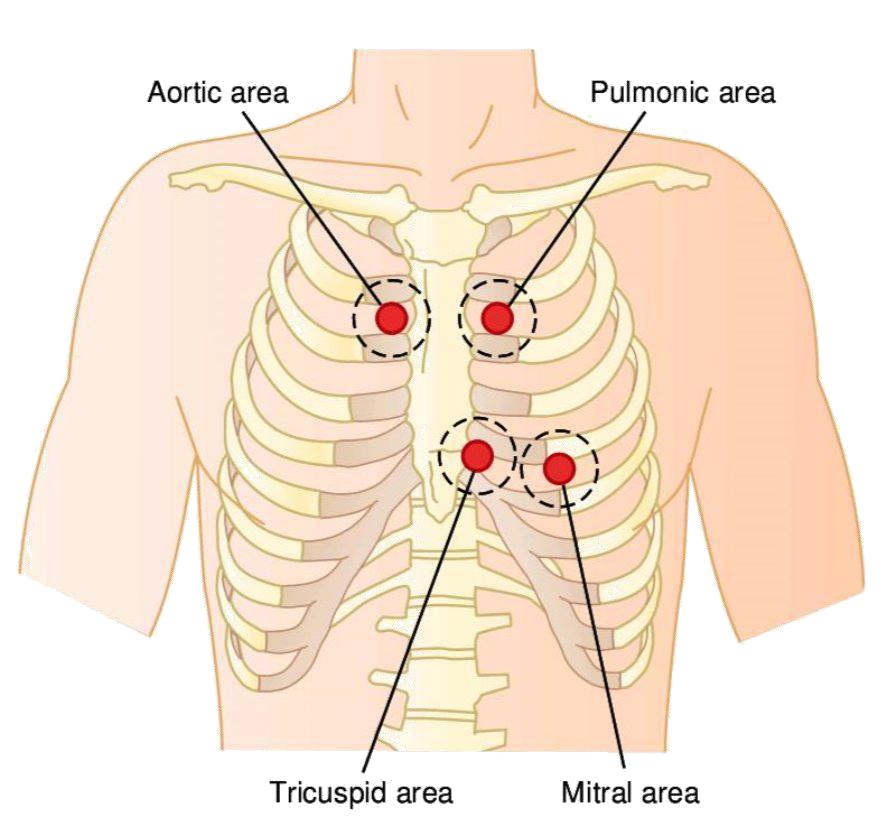
\includegraphics[width=10cm,height=15cm]{./clinicalPhysioPic/auscultatingAreas.jpg}
		\caption*{Auscultating Areas}
		\label{auscultatingAreas}
	\end{figure}
	}
Auscultate with diaphragm of the stethoscope in the following area. 
\begin{itemize}
\item[]Mitral area: Corresponds to Apical impulse (left 5th intercostals space half an inch medial to midclavicular line.
\item[]Tricuspid area: It lies close to lower end of the left border of sternum.
\item[]Aortic area: It lies in the right 2nd intercostals space close to sternum.
\item[]Pulmonary area: It lies in the left 2nd intercostals space close to sternum.
\end{itemize}
\par
While auscultating an area, feel for the carotid pulse in the neck simultaneously. The sound which coincides with the carotid pulse is the first heart sound. The heart sound that occurs in between two successive pulsations of the carotid artery is the second heart sound.
\par
1st heart sound (S1) is produced by closure of AV valves.\newline
2nd heart sound (S2) is produced by closure of semilunar valves.\newline
3rd heart sound (S3) is due to vibrations set up by rapid ventricular filling.\newline
4th heart sound (S4) is due to atrial systole.\newline
\par
First and second heart sounds are heard normally. Third heart sound is physiological in children and young adults. Fourth heart sound is not heard and can be recorded only with phonocardiogram.
\par
The second heart sound may be split. Split S2 is better appreciated in thin individuals, in pulmonary and aortic area. The Aortic component appearing before the pulmonary component.
\par
\textbf{Added sounds:} Murmurs, Opening snap, Ejection click, Pericardial rub.
\par
\textbf{Murmur:} These are abnormal sounds which are produced due to turbulence in blood flow at or near a valve or an abnormal communication within the heart. It may be systolic or diastolic or continuous.
	      \section*{Questions:}
	      \begin{enumerate}
\item{Define Apical impulse.}
\item{Mention the conditions in which the apex beat is abnormally placed.}
\item{Mention few causes for systolic and diastolic murmurs.}
\item{What are the characteristics of S1 and S2?}
\item{What is pericardial effusion?}
	      \end{enumerate}
	      %--------------------------}}}
	      %------------Recording of blood pressure ------{{{
															\chapter*{\centering Recording of Blood Pressure}
\addcontentsline{toc}{chapter}{Recording of Blood Pressure}
															\begin{tabular}{p{5in} p{1in}}
																\textbf{Exp No:}  & \textbf{Date:}\\
															\end{tabular}
															\section*{Definition:}

															Blood pressure is the lateral pressure exerted by the column of  blood on the walls of the arteries.
															\section*{Aim:}
															\addfig{%
																\centering
																\begin{figure}[H]
																	\begin{subfigure}[t]{.4\textwidth}
																	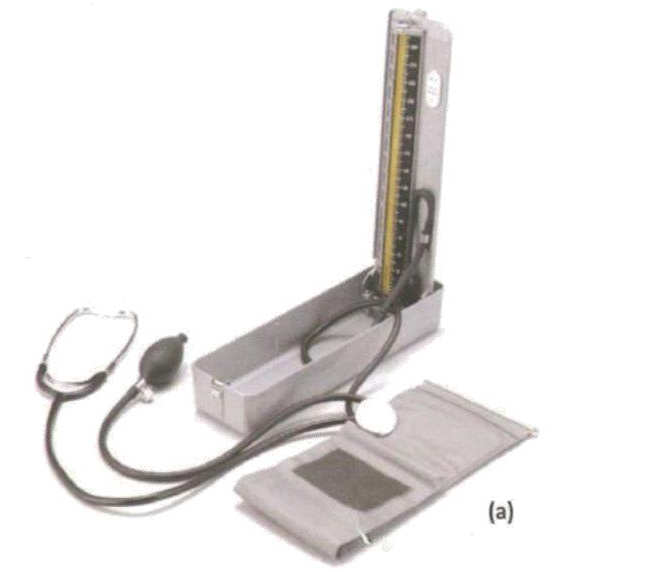
\includegraphics[width=6cm,height=6cm]{./clinicalPhysioPic/mercury_manometer.jpg}
	\subcaption{Mercury Sphygmomanometer}
																	\label{mercury_manometer}
																\end{subfigure}
																	\hspace{\fill}
																	\begin{subfigure}[t]{.4\textwidth}
																	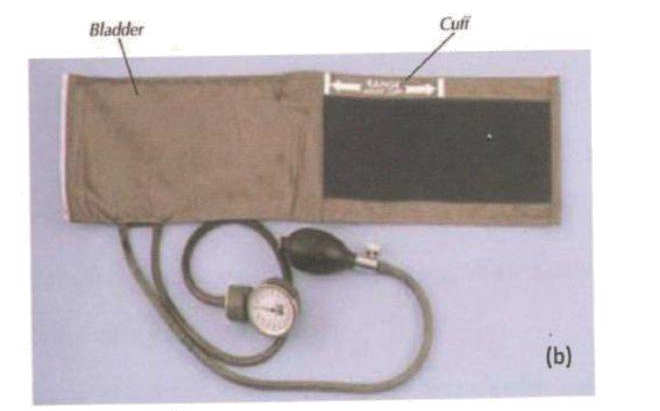
\includegraphics[width=6cm,height=6cm]{./clinicalPhysioPic/aneroid_manometer.jpg}
	\subcaption{Aneroid Sphygmomanometer}
																	\label{aneroid_manometer}
																\end{subfigure}
																\caption*{Types Of Sphygmomanometer}
																\label{Sphygmomanometer}
																\end{figure}
																}
																
To record the blood pressure of the given subject at rest.
\section*{Apparatus required :}
Sphygmomanometer and Stethoscope.
\section*{Description of Sphygmomanometer:}
The Sphygmomanometer consists of mercury manometer, cuff and air pump.
\subsection*{Mercury manometer :} It has two limbs. The broader limb is the reservoir and narrow one is graduated from 0 to 300 $mm$Hg reservoir is connected to the Riva Rocci cuff through a rubber tube.
\subsection*{Riva Rocci cuff:} It is an inflatable rubber bag .Two tubes are attached to the bag .One transmits air pressure to mercury manometer and other is connected to the air pump. The length of the rubber bag should be two thirds and its width should be one third of the mid arm circumference of the subject.
\subsection*{Airpump:} It is a rubber hand bulb provided with a one way valve and a leak valve arrangement. A rubber tube connects the air pump to the Riva Rocci cuff .The cuff can be inflated and deflated using the handpump.
\section*{Principle:}
The arterial BP is balanced against the pressure in the Riva Rocci cuff. Whenever the cuff pressure is raised above the systolic BP, the artery is occluded. When the cuff pressure becomes equal to or just below the Systolic BP, flow is restored through the artery. But the flow is turbulent. This is the reason for Korotkoff sounds. When the cuff pressure is lowered below Diastolic BP, once again streamline flow is restored and hence korotkoff sound disappears.
\section*{Procedure :}
\subsection*{Palpatory Method:}
Subject is made to sit or lie down at ease on a couch. He is allowed to rest for few minutes .The Riva Rocci Cuff is wrapped around the middle of the armo that the lower edge of the cuff is two finger breadths above the antecubital fossa. It should neither be too loose nor too tight. Zero level of the manometer should be checked. The cuff around the arm and the manometer are kept at the level of the heart to avoid the effect of gravity. Palpate the radial artery pulse.
\par
The pressure in the cuff is raised gradually until the radial pulse is no longer felt .The pressure at which the radial pulse disappears is noted .Now the pressure in the cuff is raised further and then slowly brought back by deflating the cuff. The pulse now reappears. The reading at which the pulse reappears is also noted .The disappearance and reappearance of the pulse coincides .This value is the approximate Systolic blood pressure.
\subsection*{Auscultaory method:}
The chest piece of the stethoscope is placed on the brachial artery in the antecubital fossa .The pressure in the cuff is raised to 20 to 30 mmHg above the systolic blood pressure determined by the palpatory method. While auscultating the brachial artery, the pressure in the cuff is lowered gradually .The reading in the manometer at which faint tapping sound is heard, is noted down. This is the systolic blood pressure.
\par
As the pressure in the cuff is further lowered, the sound undergoes a series of changes both in quality and intensity. Note down the reading at which the auscultatory sounds disappear. This is the diastolic blood pressure .Sometimes muffling of sounds also can be taken as diastolic BP. The ausculatory sounds heard during measurement of Blood pressure are called korotkoff’s sounds.
\paragraph{Phases of koratkoff sounds :}
\begin{itemize}
\item[]Phase I : Faint ,tapping sound .
\item[]Phase II : Sound becomes murmurish in quality .
\item[]Phase III: Sound becomes clearer and louder .
\item[]Phase IV: Sound becomes muffled. The sound then disappears.
\end{itemize}
\par
Palpatory method has to be done prior to auscultatory method because,
It gives a rough value of systolic blood pressure, It helps to avoid missing of \emph{Auscultatory gap.}
\section*{Observations}
\begin{table}[H]

		\setlength\extrarowheight{10pt}
	\begin{tabular}{|p{1.1in}|p{1.1in}|p{1.1in}|p{1.1in}|p{1.1in}|}
		\hline
		Systolic BP by palpatory method ($mm$Hg) & Systolic BP by auscultatory method ($mm$Hg) & Diastolic BP by auscultatory method ($mm$ Hg) & Pulse pressure (SBP-DBP) ($mm$ Hg) & Mean arterial pressure (DBP+${\frac{1}{3}}$ Pulse Pressure) ($mm$ Hg) \\ \hline
			                                         &                                             &                                               &                                                                              &                                                                                                               \\ \hline
								                                          &                                             &                                               &                                                                              &                                                                                                               \\ \hline
													                                           &                                             &                                               &                                                                              &                                                                                                               \\ \hline
	\end{tabular}
\end{table}
%-----------------------}}}
%------------Effect of posture and exercise on BP--{{{
															\chapter*{\centering Effects of Posture and Exercise on	Blood Pressure}
\addcontentsline{toc}{chapter}{Effects of Posture and Exercise on	Blood Pressure}
															\begin{tabular}{p{5in} p{1in}}
																\textbf{Exp No:}  & \textbf{Date:}\\
															\end{tabular}
\section*{Aim:}
	To record the effects of changes in posture and physical exercise on blood pressure.
	\section*{Apparatus required :}
	Sphygmomanometer and stethoscope
	\section*{Effect Of Changes In Posture On Blood Pressure}
	\subsection*{Procedure:}
	\begin{itemize}
\item{The subject should be mentally and physically relaxed.}
\item{Record resting blood pressure of the subject in supine posture by palpatory and ausculatory method.}
\item{The deflated cuff is still wrapped around his arm.}
\item{Now the subject is instructed to stand up swiftly from the lying posture and to lean against a support (the couch).}
\item{Immediately record his blood pressure by auscultatory method.}
\item{Record blood pressure again at the end of 2min and 5min on standing.}
	\end{itemize}
	\subsection*{Discussion:}
		When an individual stands up immediately from recumbent posture, there is pooling of blood in the legs.
		The venous return to the heart is reduced thereby reducing the cardiac output. Hence, the systolic blood pressure will fall, which may be recorded within 15seconds. This will be brought back to normal by Baroreceptor reflex within 15 to 30 seconds .Hence, a fall in systolic BP is usually difficult to record in normal subjects.
		This is a function of autonomic nervous system (ANS).
		\subsection*{Observation - Effect Of Change in Posture on BP}
\begin{table}[H]
	\setlength\extrarowheight{15pt}
\begin{tabular}{|p{1.2in}|p{1.2in}|p{1.2in}|p{1.2in}|}
	\hline
	Posture                                                           & Systolic BP by palpatory method ($mm$Hg) & Systolic BP by auscultatory method ($mm$ Hg) & Diastolic BP by auscultatory method ($mm$ Hg) \\ \hline
	Supine                                                            &                                          &                                              &                                               \\ \hline
	\begin{tabular}[c]{@{}l@{}}Immediately\\ on standing\end{tabular} & Not to be done                           &                                              &                                               \\ \hline
		2 min                                                             & Not to be done                           &                                              &                                               \\ \hline
		5 min                                                             & Not to be done                           &                                              &                                               \\ \hline
\end{tabular}
\end{table}
	\section*{Effect Of Exercise On Blood Pressure}
\subsection*{Procedure:}
\begin{itemize}
\item{Record resting blood pressure in sitting posture by palpatory and ausculatory method.}
\item{The Riva Rocci cuff is disconnected from the BP apparatus.}
\item{The cuff is still wrapped around the subject’s arm.}
\item{The subject is instructed to perform physical activities like on the spot jogging for five minutes or ten sit ups}
\item{Immediately after the exercise, BP is recorded by auscultaory method without any time delay.}
\end{itemize}

\subsection*{Discussion:}
Systolic BP will show a rise due to increase in the heart rate and cardiac output. This is due to increased activity of sympathetic nervous system .Diastolic BP will not change in mild to moderate exercise. In severe exercise, diastolic BP may fall due to local vasodilatation in working muscles which will decrease the peripheral resistance.

\subsection*{Observation - Effect Of Exercise On Blood Pressure}
\begin{table}[H]
	\setlength\extrarowheight{25pt}
	\begin{tabular}{|p{1.2in}|p{1.2in}|p{1.2in}|p{1.2in}|}
		\hline
		                                                                     & Systolic BP by palpatory method ($mm$Hg) & Systolic BP by auscultatory method ($mm$ Hg) & Diastolic BP by auscultatory method ($mm$ Hg) \\ \hline

										     BP at rest                                                           &                                          &                                              &                                               \\ \hline
										     \begin{tabular}[c]{@{}l@{}}Immediately\\ after exercise\end{tabular} & Not to be done                           &                                              &                                               \\ \hline
											     2 min after exercise                                                 & Not to be done                           &                                              &                                               \\ \hline
											     5 min after exercise                                                 & Not to be done                           &                                              &                                               \\ \hline
	\end{tabular}
\end{table}
\section*{Questions:}
\begin{enumerate}
\item{Define Blood pressure.}
\item{What is pulse pressure ?}
\item{How will you calculate Mean arterial pressure.?}
\item{What is the importance of palpatory method ?}
\item{What is an auscultatory gap?}
\item{What are korotkoff’s sounds?}
\item{What is postural hypotension?}
\end{enumerate}
%----------}}}
%-----------------Examination of sensory system----{{{

															\chapter*{\centering Examination Of Sensory System}
\addcontentsline{toc}{chapter}{Examination Of Sensory System}
															\begin{tabular}{p{5in} p{1in}}
																\textbf{Exp No:}  & \textbf{Date:}\\
															\end{tabular}
															\section*{Pre-requisites for the examination}
			\addfig{%
				\centering
				\begin{figure}[H]
					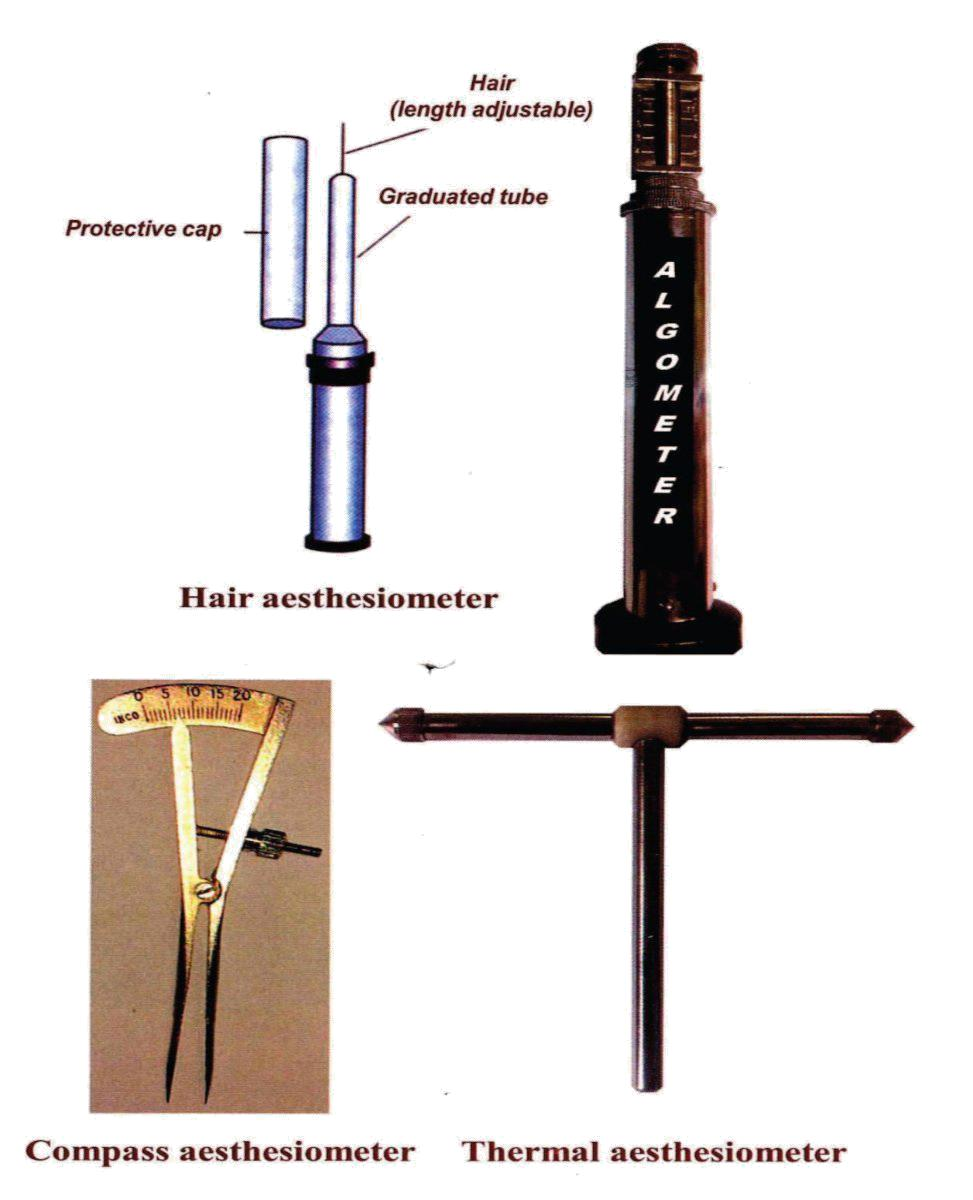
\includegraphics[height=18cm,width=12cm]{./clinicalPhysioPic/sensoryIntruments.jpg}
					\label{SensoryIntruments}
				\end{figure}
				}												\par									Before starting the procedure explain the nature of the test to be performed. Ask the subject to close the eyes or turn the face to the other side whenever necessary.
															\par
Apply uniform sensory stimulus and examine dermatome wise on both sides.
\paragraph{Following sensations are tested}
\begin{itemize}
\item{Tactile sensation - light touch, crude touch, tactile localisation and 	discrimination}
\item{Position sense:}
\item{Vibration sense}
\item{Pain – superficial and deep}
\item{Temperature sense- warmth and cold}
\item{Stereognosis:}
\item{Romberg’s sign}
\end{itemize}
\subsection*{TACTILE SENSATION: (Tested with eyes closed)}
\subsubsection*{Fine touch (Light touch):}
\begin{itemize}
\item{ Ask the subject to say ‘yes’ or raise his finger when he perceives the sensation of touch.}
\item{ With a wisp of cotton wool, lightly touch the different parts of the body and compare with the corresponding area on the opposite side dermatome wise}
\item{ Also enquire whether he perceives it normally or differently.}
\item{ It can also be elicited by Von frey’s hair aesthesiometer.}
\end{itemize}

\subsubsection*{Crude touch (Pressure sense):}
\begin{itemize}
\item{Pressure is the sustained touch sensation.}
\item{Elicit the pressure sensation by pressing with your finger tip on 	corresponding areas of both sides dermatome wise}
\end{itemize}

\subsubsection*{Tactile localisation:}
\begin{itemize}
\item{It is the ability to localise the touch with a ball pen tip.}
\item{Measure the distance between the two points (localisation distance).  Tested in all dermatomes on both sides.}
\item{Localisation distance varies in different parts of the body. It corresponds with the density of touch receptors.}
\end{itemize}

\subsubsection*{Two point discrimination:}
\begin{itemize}
\item{Instruction is given to the subject to say whether he feels the touch as one point or two points when he is touched by a compass aesthesiometer}
\item{Start with minimum distance of 1$mm$, touch the skin of the subject lightly with the two points simultaneously.}
\item{Ask the subject to say whether he is being touched by one or two points.}
\item{If the subject says one, increase the distance gradually till two separate points are appreciated by him. This is the minimum separable distance.}
\item{Record the minimum separable distance on different parts of the body on both the sides.}
\end{itemize}
\par
(Minimum separable distance varies in different parts of the body - about 2$mm$ on finger tips, 5$mm$ on hands and maximum on the back of the trunk which is about 5$cm$. This is due to the difference in distribution of sensory receptive fields.)
\begin{itemize}
\item[]Anaesthesia 	– loss of all sensations
\item[]Hypoaesthesia 	– Reduced touch sensation
\item[]Hyperaesthesia 	- When the response to the sensory stimulus is exaggerated.  eg.thalamic lesion
\item[]Paraesthesia 	- Perverted touch sensation (Touch may produce unpleasant 				sensation)
\end{itemize}

\subsection*{SENSE OF POSITION: (to be done with eyes closed)}
\par
The appreciation of passive movement
\par
	Hold the finger and fix the interphalangeal joint. Passively flex and extend the finger holding the joint, and leave it in some definite position . Ask the subject to keep the corresponding finger in similar position .Perform the test on all the upper and lower limb small and large.
	\par
(Movements of less than 10${^\circ}$ are appreciated at all the normal joints).
\subsection*{VIBRATION SENSE: (to be done with eyes closed)}
\begin{itemize}
\item{over bony prominences like styloid process of the radius ,the lower end of the tibia, and medial or l ateral malleolus.}
\item{Ask the subject if he perceives vibrations and instruct him to raise his hand when he ceases to feel the vibration.}
\item{Immediately place tuning fork on the corresponding bony prominence of the examiner. If the examiner can still perceive it, the subject's perception of vibration is impaired.}
\end{itemize}
\subsection*{PAIN SENSATION (to be done with eyes open)}
\addfig{%
	\centering
	\begin{figure}[H]
		\begin{subfigure}[t]{.43\textwidth}
			\centering
			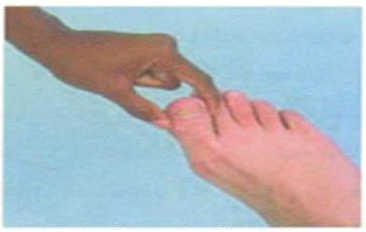
\includegraphics[width=5cm,height=5cm]{./clinicalPhysioPic/positionSense.jpg}
			\subcaption{Position Sense}
			\label{position sense}
		\end{subfigure}
		\hspace{\fill}
		\begin{subfigure}[t]{.43\textwidth}
			\centering
			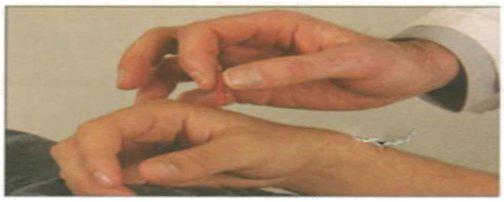
\includegraphics[width=5cm,height=5cm]{./clinicalPhysioPic/painSense.jpg}
			\subcaption{Pain Sense}
			\label{pain sense}
		\end{subfigure}
		\hspace{\fill}
		\begin{subfigure}[t]{.43\textwidth}
			\centering
			\includegraphics[width=5cm,height=5cm]{./clinicalPhysioPic/twoPointDiscrimination.jpg}
			\subcaption{Two Point Discrimination}
			\label{twoPointDiscrimination}
		\end{subfigure}
		\hspace{\fill}
		\begin{subfigure}[t]{.43\textwidth}
			\centering
			\includegraphics[width=5cm,height=5cm]{./clinicalPhysioPic/sensorySystem2.jpg}
			\subcaption{Vibration Sense}
			\label{vibrationSense}
		\end{subfigure}
		\caption*{Sensory System Examination}
		
	\end{figure}
	}
\subsubsection*{Superficial pain:}
\begin{itemize}
\item{Explain the procedure}
\item{Elicit superficial pain by gently pricking the skin with a pin}
\item{Ask the subject if he perceives the pain}
\item{Test pain in all the dermatomes on both sides.}
\end{itemize}
\subsubsection*{Deep pain:}
	Elicit Deep pain by squeezing the deeper structures such as the muscle or the tendon. It can also be quantified using Algometer.
	\begin{itemize}
\item{Analgesia is loss of pain sensation}
\item{Hypoalgesia is partial loss of pain sensibility}
\item{Hyperalgesia is a condition of exaggerated sensibility to pain}
	\end{itemize}
	\subsection*{THERMAL SENSE:}
	\begin{itemize}
\item{Take two test tubes containing warm and cold water separately}
\item{Give proper instructions to the subject (to say whether he feels cold or warm when touched with different glass tubes)}
\item{Place the bottom of the test tubes on the skin of the subject each ‘in turn or randomly’ and ask the subject to say what he feels}
\item{Test and compare all the dermatomes.}
	\end{itemize}
	\subsection*{STEREOGNOSIS: (to be done with eyes closed)}
\begin{itemize}
\item{Place a familiar object in subject’s hand}
\item{The subject should identify the object by its shape,texture, size, etc and should tell what it is}
\item{Repeat the procedure with 4 to 5 familiar objects}
\item{Repeat the procedure in the other hand}
	\end{itemize}
	\par
	Ability to recognize the known objects purely from the feel of its shape and size with eyes closed is called stereognosis.
	\par
	Tactile localization, tactile discrimination and stereognosis are known as cortical sensations as intact parietal association area is needed.
\subsection*{ROMBERG’S SIGN:}
\par
	Ask the subject to stand with his feet close together and then to close his eyes. Swaying of the body from side to side will occur if the posterior column is affected. The position sense from the legs is lacking, hence the subject becomes unsteady on closing the eyes.
	\par
	This is a test for the loss of position sense (sensory ataxia) in the legs. It is not at a test for cerebellar function. This is a test to differentiate sensory ataxia from cerebellar ataxia. In cerebellar ataxia, the subject is unsteady with his feet together even with eyes open.

	\begin{table}[H]
\centering
		\begin{tabular}{|p{1in}|p{1.75in}|p{1.75in}|}
\hline
S.No. & \textbf{Senses}                                                                                       & \textbf{Carried by the Tracts}  \\
\hline
1     & Fine touch,Tactile localization, Tactile discrimination, position sense, vibration sense and stereognosis & Dorsal/ posterior column       \\
\hline
2     & Crudetouch                                                                                            & Anteriorspinothalamic tract    \\
\hline
3     & Pain\& Temperature                                                                                    & Lateralspino-thalamic tract    \\
\hline
\end{tabular}
\end{table}

\section*{Inference :}
\vspace{2in}



\section*{Questions:}
\begin{enumerate}
\item{What is a dermatome?}
\item{Name the receptors for pain.}
\item{What are the types of pain?}
\item{Name the sensations lost in posterior column lesions of the spinalcord.}
\item{What are cortical sensations?.}
\item{What are Brodmann’s area numbers for primary and secondary sensory area?}
\item{What is the frequency of the tuning fork used to test vibration sense?}
\item{What is astereognosis?}
\end{enumerate}

\newpage
{\centering \paragraph{Clinical Examination of Sensory System}}
															\begin{tabular}{p{5in} p{1in}}
																\textbf{Name:}  & \textbf{Age:}\\
																\textbf{Sex:} & \textbf{Occupation:}
															\end{tabular}
															% Please add the following required packages to your document preamble:
% \usepackage{multirow}
% \usepackage{graphicx}
															\renewcommand{\arraystretch}{2}
\begin{table}[H]
\resizebox{\textwidth}{!}{%
\begin{tabular}{|c|c|c|c|c|c|c|c|c|}
\hline
\multirow{2}{*}{\textbf{Sensation}} & \multicolumn{2}{c|}{\textbf{Cervical}} & \multicolumn{2}{c|}{\textbf{Thoracic}} & \multicolumn{2}{c|}{\textbf{Lumbar}} & \multicolumn{2}{c|}{\textbf{Sacral}} \\ \cline{2-9}
                                    & \textbf{Right}     & \textbf{Left}     & \textbf{Right}     & \textbf{Left}     & \textbf{Right}    & \textbf{Left}    & \textbf{Right}    & \textbf{Left}    \\ \hline
Fine touch                          &                    &                   &                    &                   &                   &                  &                   &                  \\ \hline
Crude touch                         &                    &                   &                    &                   &                   &                  &                   &                  \\ \hline
Tactile localisation                &                    &                   &                    &                   &                   &                  &                   &                  \\ \hline
Joint \& Position sense             &                    &                   &                    &                   &                   &                  &                   &                  \\ \hline
Vibration                           &                    &                   &                    &                   &                   &                  &                   &                  \\ \hline
Superficial pain                    &                    &                   &                    &                   &                   &                  &                   &                  \\ \hline
Temperature (warmth)                &                    &                   &                    &                   &                   &                  &                   &                  \\ \hline
Temperature (cold)                  &                    &                   &                    &                   &                   &                  &                   &                  \\ \hline
Steregnosis                         &                    &                   &                    &                   &                   &                  &                   &                  \\ \hline
Romberg's sign                      & \multicolumn{8}{c|}{}                                                                                                                                         \\ \hline
\end{tabular}%
}
\end{table}
\renewcommand{\arraystretch}{1}
%------------------------}}}
%------------Examination of motor system-----------{{{
															\chapter*{\centering Examination Of Motor System}
\addcontentsline{toc}{chapter}{Examination Of Motor System}
															\begin{tabular}{p{5in} p{1in}}
																\textbf{Exp No:}  & \textbf{Date:}\\
															\end{tabular}
															\section*{Introduction}
Examination of the motor system is carried out by assessing,
\begin{itemize}
\item{Nutrition or bulk of the muscle}
\item{Tone of the muscle}
\item{Power or strength of the muscle}
\item{Co-ordination of movements}
\item{Reflexes}
\item{Gait}
\item{Involuntary movements}
\end{itemize}

\section*{Nutrition Or Bulk Of The Muscle:}
\addfig{
	\begin{figure}[H]
		\begin{subfigure}[t]{.25\textwidth}
			\includegraphics[width=5cm,height=5cm]{./clinicalPhysioPic/motorSystem/abductorPollicisBrevis.jpg}
			\subcaption{Testing abductor Pollicis brevis}
		\end{subfigure}
		\hspace{\fill}
		\begin{subfigure}[t]{.25\textwidth}
			\includegraphics[width=5cm,height=5cm]{./clinicalPhysioPic/motorSystem/opponensPollicis.jpg}
			\subcaption{Testing opponens pollicis}
		\end{subfigure}
		\hspace{\fill}
		\begin{subfigure}[t]{.25\textwidth}
			\includegraphics[width=5cm,height=5cm]{./clinicalPhysioPic/motorSystem/interossesi.jpg}
			\subcaption{Testing Dorsal and palmar interossei}
		\end{subfigure}
		\hspace{\fill}
		\begin{subfigure}[t]{.25\textwidth}
			\includegraphics[width=5cm,height=5cm]{./clinicalPhysioPic/motorSystem/flexorArm.jpg}
			\subcaption{Testing Biceps}
		\end{subfigure}
		\hspace{\fill}
		\begin{subfigure}[t]{.25\textwidth}
			\includegraphics[width=5cm,height=5cm]{./clinicalPhysioPic/motorSystem/extensorArm.jpg}
			\subcaption{Testing Triceps}
		\end{subfigure}
		\hspace{\fill}
		\begin{subfigure}[t]{.25\textwidth}
			\includegraphics[width=5cm,height=5cm]{./clinicalPhysioPic/motorSystem/deltoid.jpg}
			\subcaption{Testing Deltoid}
		\end{subfigure}
		\hspace{\fill}
		\begin{subfigure}[t]{.25\textwidth}
			\includegraphics[width=5cm,height=5cm]{./clinicalPhysioPic/motorSystem/supraspinatus.jpg}
			\subcaption{Testing Supraspinatus:}
		\end{subfigure}
		\hspace{\fill}
		\begin{subfigure}[t]{.25\textwidth}
			\includegraphics[width=5cm,height=5cm]{./clinicalPhysioPic/motorSystem/infraspinatus.jpg}
			\subcaption{Testing Infraspinatus:}
		\end{subfigure}
		\hspace{\fill}
		\begin{subfigure}[t]{.25\textwidth}
			\includegraphics[width=5cm,height=5cm]{./clinicalPhysioPic/motorSystem/pectoralisMajor.jpg}
			\subcaption{Testing Pectoralis Major}
		\end{subfigure}
		\hspace{\fill}
		\begin{subfigure}[t]{.25\textwidth}
			\includegraphics[width=5cm,height=5cm]{./clinicalPhysioPic/motorSystem/hipFlexion.jpg}
			\subcaption{Testing hip flexors}
		\end{subfigure}
		\hspace{\fill}
		\begin{subfigure}[t]{.25\textwidth}
			\includegraphics[width=5cm,height=5cm]{./clinicalPhysioPic/motorSystem/hipExtension.jpg}
			\subcaption{Testing hip extensors}
		\end{subfigure}
		\hspace{\fill}
		\begin{subfigure}[t]{.25\textwidth}
			\includegraphics[width=5cm,height=5cm]{./clinicalPhysioPic/motorSystem/hipAbduction.jpg}
			\subcaption{Testing hip Abductors}
		\end{subfigure}
		\caption*{Examination Of Muscle Power}
	\end{figure}
}
\begin{itemize}
\item{Inspect the different groups of muscles of the body on both sides for any wasting or contractures.}
\item{Palpate the muscles and feel for the consistency. Atrophic muscle appears smaller and feels soft and flabby. Hypertrophic muscle appears bulky and are firm in consistency.}
\item{Bulk of the muscle is assessed by measuring the circumference of the limbs at point of maximum bulk with reference to a definite bony landmark using an inch tape.}
\item{Bony landmarks}
	\begin{itemize}
		\item[]Upper limb 	–	Arm circumference with reference to acromian or olecranon 			process. Forearm circumference with reference to olecranon 			process.
		\item[]Lower limb 	–	Thigh and leg circumference with reference to tibial 				tuberosity. 
	\end{itemize}
\item{ Compare the bulk of both limbs at the same reference point.}
\end{itemize}

\section*{Tone:}
	Muscle tone is a state of partial contraction of muscle at rest.
	\begin{itemize}
\item{Ask the subject to keep the limb relaxed. Hold the limb and do passive movements on various joints and observe the degree of resistance offered by the muscle.}
\item{The degree of resistance offered by the muscle indicates the tone of the muscle.}
\item{Compare the tone of the muscles on both sides.}
	\end{itemize}
	\par
	Hypertonia is increase in muscle tone. It is seen in upper motor neuron lesions. It is of two types: spasticity and rigidity.
	\begin{itemize}
		\item{\textbf{Spasticity:} Hypertonia of the corticospinal tract lesion is of Clasp knife type and it involves one group of muscles either the agonist or the antagonist muscles. It is maximum in the flexors of the upper limb and extensors of the lower limb.}
		\item{\textbf{Rigidity:} Hypertonia of the extrapyramidal tracts lesion, involves both the agonist and the antagonist muscles. In Cog wheel rigidity, the resistance offered is intermittent. In Lead pipe rigidity, the resistance is felt throughout the range of movement.}
	\end{itemize}
	Hypotonia is decrease in muscle tone. It is seen in lower motor neuron lesions. Eg: Poliomyelitis and cerebellar lesions.
	\section*{Power Or Strength Of The Muscles:}
	\begin{itemize}
\item{Expose the muscle to be tested. Ask the subject to perform the movement as instructed and offer resistance. Observe the contraction of the muscle. Compare strength of same group of muscle on the other side}
\item{The strength of the muscle is assessed by comparing the  strength of the examiner.}
	\end{itemize}
	\subsection*{Grading of power:}
	\par
	\begin{align*}
		\text{Grade 0} 	&:	\text{Complete paralysis.} \\
	\text{Grade 1} 	&: 	\text{Flicker of contraction only.}\\
		\text{Grade 2} 	&: \text{Muscle movement only when gravity is eliminated}\\
	\text{Grade 3} 	&:	\text{Muscle movement against the force of gravity, but not against resistance.} \\
	\text{Grade 4} 	&:	\text{Some degree of weakness, usually described as poor, fair or moderate 		strength.} \\
	\text{Grade 5} 	&:	\text{Normal power.}\\
	\end{align*}


	\subsection*{Testing muscles of the upper limb:}
	\begin{enumerate}
\item{ Abductor pollicis brevis:
	\par
	Ask the subject to abduct the thumb against resistance in a plane at right angle to the palmar aspect of the index finger.
}
\item{ Opponens pollicis:
	\addfig{
		\begin{figure}[H]
		\begin{subfigure}[t]{\textwidth}
			\centering
			\includegraphics[width=5cm,height=5cm]{./clinicalPhysioPic/motorSystem/hipAdduction.jpg}
			\subcaption{Testing hip Adductors}
		\end{subfigure}
		\hspace{\fill}
		\begin{subfigure}[t]{\textwidth}
			\centering
			\includegraphics[width=5cm,height=5cm]{./clinicalPhysioPic/motorSystem/kneeFlexion.jpg}
			\subcaption{Testing hip Adductors}
		\end{subfigure}
		\hspace{\fill}
		\begin{subfigure}[t]{\textwidth}
			\centering
			\includegraphics[width=5cm,height=5cm]{./clinicalPhysioPic/motorSystem/kneeExtension.jpg}
			\subcaption{Testing hip Adductors}
		\end{subfigure}
		\hspace{\fill}
			\caption*{Examination Of Muscle Power}
		\end{figure}
		}
	\par
	Ask the subject to touch the tip of his little finger with the point of his thumb against resistance without moving the little finger.
}
\item{ First dorsal interosseous:
	\par
	Ask the subject to abduct his index finger against resistance.
}
\item{ Interossei and lumbricals: Dorsal interossei:
	\par
	Ask the subject to abduct the fingers against resistance. The dorsal interossei causes the abduction of the fingers at the metacarpophalangeal joint.
}
\item{	Palmar interossei:
	\par
	Place the paper between the fingers and ask the subject to hold it. Try to pull the paper out. The palmar interossei causes adduction of the fingers at the metacarpophalangeal joint.
			}
\item{Lumbricals:
	\par
	Ask the subject to flex the metacarpophalangeal joints and to extend the distal interphalangeal joints against resistance.
}
\item{ Flexors of the fingers: 
\par
Ask the subject to squeeze the examiner's index and middle fingers on both sides and assess the force of grip.
}
\item{ Flexors of the wrist: 
\par
Ask the subject to flex the wrist against resistance.
}
\item{ Extensors of the wrist: 
\par
Ask the subject to make a fist and hold the hand with palm facing downwards. Offer resistance when the subject is asked to extend the wrist.
}
\item{ Brachio-radialis: 
\par
Ask the subject to place the forearm in mid prone position, and flex the forearm. Offer resistance by grasping the hand.
}
\item{ Biceps: 
\par
With the forearm in full supination, ask the subject to flex the forearm against resistance.
}
\item{ Triceps: 
\par
The subject is asked to extend the flexed forearm against resistance.
}
\item{ Supraspinatus: 
\par
Ask the subject to keep the arm by the side of the body and to lift his arm at right angles to his side against resistance. The first 300of abduction is carried out by supraspinatus. The remaining 600 is by the deltoid.
}
\item{ Deltoid: 
\par
Ask the subject to make forward and backward movement of the abducted arm against resistance.
}
\item{ Infraspinatus: 
\par
Ask the subject to flex the forearm at right angle and tuck the elbow to his side. Ask to rotate his forearm outwards against resistance. The elbow has to be tucked to the side throughout.
}
\item{ Pectoralis: 
\par
Ask the subject to stretch his arms out in front of him and to clasp his hands together while the examiner attempts to hold them apart.
}
\item{ Serratus anterior: 
\par
Ask the subject to push forward his hands against a wall. If there is paralysis of serratus anterior, winging of scapula occurs on that side.
}
\item{ Lattisimus dorsi: 
\par
Ask the subject to clasp his hands behind his back while the examiner stands behind him and offers passive resistance.
}	
\end{enumerate}
\subsection*{Muscles	of	the	trunk:}	
\subsubsection*{Abdominal muscles:}
	With the subject in supine position, ask the subject to lift up his head against resistance. In paralysis of lower abdominal segment, umbilicus moves up. When the upper segment is paralysed umbilicus is pulled down. This is called Beevor's sign.
	\par
	In weakness of the abdominal muscles, the subject will not be able to sit up in bed from the supine position without the aid of his hands(Babinski’s rising up sign).
	\subsubsection*{Muscles of the back: (Erector spinae).}
	Ask the subject to lie with his face down and to raise his head from the bed by extending his neck and the back. Muscles of the back stand out prominently.
\subsection*{Muscles of lower limb:}
\begin{enumerate}
\item{Muscles of foot and toes:}
\begin{itemize}
	\item{Dorsi-flexors and plantar flexors of the feet and toes:
		\par
Ask the subject to dorsiflex and plantarflex the distal foot against resistance.
		}
	\item{Evertors and invertors:
		\par
Ask the subject to evert and invert against resistance. Eversion and inversion takes place at the subtalar joint.
		}
\end{itemize}
\item{Extensors of knee:
	\par
In supine position, ask the subject to flex his knee and to extend the leg while offering resistance on the shin just above the ankle.
		}
\item{Flexors of knee:
	\par
Raise the leg up from the bed, supporting the thigh with your left hand and holding the ankle with your right hand, ask the subject to bend his knee
		}
\item{ Extensors of hip: 
\par
With the limb fully extended, lift the subject’s foot off the bed, and ask him to bring the limb down to the bed against resistance.
}

\item{ Flexors of thigh: 
\par

With the leg extended, ask the subject, to raise his leg off the bed against resistance without bending the knee. Resistance is given just above the ankle joint.
}

\item{ Abductors of thigh: 
\par
With the legs placed together in the midline, ask the subject to abduct his legs against resistance.
}

\item{ Adductors of thigh: 
\par
With the legs kept apart, ask the subject to bring the legs to midline against resistance.
}

\item{ Rotators of the thigh or hip:
	\par
With the lower limbs extended on the bed, ask the subject to rotate the limb outwards or inwards against resistance.
}
\end{enumerate}

\section*{Co-ordination:} 
\emph{(refer experiment- Cerebellar function test)}
\section*{Reflexes:}
\emph{(refer experiment- Reflexes)}
\section*{Gait:}
Ask the subject to walk barefoot in a straight line, and to turn round at a given point and then to come back. While walking, observe whether he walks in a straight line and if he deviates in any direction. Observe for automatic associated movements. .
\begin{itemize}
\item{Festinant gait in Parkinson's disease.}
\item{Waddling gait in muscular dystrophy and myopathies.}
\item{High stepping gait in common peroneal nerve palsy.}
\end{itemize}

	\section*{Involuntary Movements:}

\subsection*{Tremor:}
Tremor is a regular, rhythmic, purposeless to and fro movement of a part of the body due to alternate contraction and relaxation of the agonist and antagonist muscles. It is of two types. Fine tremor and coarse tremor

\subsubsection*{Causes of tremor:}
Physiological: Anxiety, old age and exposure to cold\\
Pathological: Parkinsonism, cerebellar disorders, thyrotoxicosis,  	hypoglycaemia, alcoholism and heavy metal poisoning.
\subsection*{Myoclonus:}
	Sudden shock like contraction of a single muscle or a group of muscles. 
	\subsection*{Athetosis:}
		It is characterized by slow, worm like writhing movements of the extremities affecting chiefly the fingers and the wrist. Seen in lesion of Globus pallidus.
		\subsection*{Chorea:}
			It is characterized by brisk, jerky, purposeless and graceful movements of the distal part of the extremities and is usually associated with twitching of the face. Seen in Huntington's disease and Rheumatic heart disease.
			\subsection*{Ballismus:}
				It is a rare involuntary movement characterized by a sudden violent movement of the body. Occurs in lesion of subthalamic nucleus. When it occurs in one half of the body it is called hemiballismus.
				\subsection*{Ticks:}
				Sudden, rapid, repeated, coordinated and purposeless movements that occur in the form of blinking of the eyes or wriggling of the shoulders.
				\section*{Questions:}
				\begin{enumerate}
\item{Define muscle tone.}
\item{Define hemiparesis, hemiplegia and paraplegia.}
\item{Name the descending tract that controls voluntary motor movements?}
\item{Name the extra-pyramidal tracts.}
\item{What are the differences between UMN lesion and LMN lesion?}
\item{List out the differences between spasticity and rigidity.}
				\end{enumerate}
\section*{Inference:}
\vspace{2in}
%-------------------------------}}}
%------------------Reflexes-----{{{
															\chapter*{\centering Reflexes}
\addcontentsline{toc}{chapter}{Reflexes}
															\begin{tabular}{p{5in} p{1in}}
																\textbf{Exp No:}  & \textbf{Date:}\\
															\end{tabular}
															\section*{Definition:}
															\addfig{
																\begin{figure}[H]
																	\centering
																	\includegraphics[width=10cm,height=15cm]{./clinicalPhysioPic/reflexes/reflexArc.jpg}
																\end{figure}
																}
Reflex is an automatic (involuntary) response to a stimulus. The response depends on the integrity of the reflex arc and is influenced by the higher centres.
\paragraph{Components Of Reflex Arc:}
\begin{enumerate}
\item{ Receptor}
\item{ Afferent}
\item{ Centre}
\item{ Efferent}
\item{ Effector organ}
\end{enumerate}
\paragraph{Types Of Reflexes:}
\begin{itemize}
\item{Superficial reflexes}
\item{Deep reflexes}
\item{Visceral reflexes}
\end{itemize}
\section*{Aim:} 
To elicit superficial, deep and visceral reflexes in the subject.
\section*{Apparatus Required:}
Knee hammer, cotton swab.
\section*{Superficial Reflexes: }
These are 'polysynaptic reflexes'.
\begin{itemize}
\item{Stimulus: Superficial structure. ( skin / mucous membrane)}
\item{Response: Contraction of underlying muscles.}
\item{Pathway:}
	\begin{itemize}
\item{Afferent - Sensory nerve (component of mixed nerve)}
\item{Center - Spinal cord or brainstem or forebrain.}
\item{Efferent - Motor nerve (component of mixed nerve) to underlying muscles.}
	\end{itemize}
\end{itemize}
\subsection*{Conjunctival reflex:}
	Ask the subject to look at a distant object. Touch the bulbar conjunctiva with a fine wisp of sterile cotton brought from the side. Test both the eyes.\newline
\textbf{Response}: Closure of both eyes.\\  
\textbf{Afferent}– 5th cranial nerve. \textbf{Efferent} – 7th cranial nerve.
\subsection*{Corneal reflex:}
Ask the subject to look at a distant object. Then touch the limbus (sclerocorneal junction) with a sterile cotton wool brought from the side of the subject. Test both the eyes.\\
\textbf{Response:}Closure of both eyes.\\
\textbf{Afferent}– 5th cranial nerve. \textbf{Efferent}– 7th cranial nerve.
\subsection*{Abdominal Reflex: (T7- T12)}
Ask the subject to lie in supine position with abdomen uncovered.\\
\textbf{Stimulus}: With the blunt end of the knee hammer, stroke lightly and briskly on each quadrant of abdomen above and below the umbilicus from outer aspect towards midline.\\
\textbf{Response}: Contraction of abdominal muscles in that quadrant.
\subsection*{Plantar Reflex: (L5, SI)}
Ask the subject to lie in supine position with the muscles of lower limbs completely relaxed.\\
\textbf{Stimulus}: With the blunt end of the knee hammer, outer edge of the sole of foot is stroked gently along the lateral border starting from heel towards little toe and then along the bases of other toes medially.\\
\textbf{Normal Response: }\\
"Extensor plantar response" manifested by
\begin{itemize}
\item{Plantar flexion of all the toes at metatarsophalangeal and inter phalangealjoints.}
\item{Inversion and plantar flexion of ankle.}
\end{itemize}
\textbf{Abnormal Response:}\\
"Extensor plantar response" manifested by
\addfig{
	\begin{figure}[H]
		\begin{subfigure}[t]{.4\textwidth}
			\includegraphics[width=5cm,height=5cm]{./clinicalPhysioPic/reflexes/cornealReflex.jpg}	
			\subcaption{Corneal Reflex}
		\end{subfigure}
		\hspace{\fill}
		\begin{subfigure}[t]{.4\textwidth}
			\includegraphics[width=5cm,height=5cm]{./clinicalPhysioPic/reflexes/abdominalReflex.jpg}
			\subcaption{Abdominal Reflex}	
		\end{subfigure}
		\hspace{\fill}
		\begin{subfigure}[t]{\textwidth}
			\centering
			\includegraphics[width=10cm,height=5cm]{./clinicalPhysioPic/reflexes/plantarRelfex.jpg}	
			\subcaption{Normal And Abnormal Plantar responses}
		\end{subfigure}
		\hspace{\fill}
		\caption*{Superficial Reflexes}
	\end{figure}
}
\begin{itemize}
\item{Dorsiflexion of great toe with abduction and fanning out of other toes.}
\item{Eversion and dorsiflexion of ankle.}
\item{Also called as Babinsk's sign.}
\item{The diagnostic feature of UMN lesion especially corticospinal tract lesion.}
\item{Normally seen in newborns and infants (primitive reflex), sleep and deep anaesthesia.}
\end{itemize}
\subsection*{Other reflexes:}
\begin{itemize}
\item{Scapular reflex: C5-T1.}
\item{Anal reflex: S3-S4.}
\item{Cremasteric reflex: LI - L2.}
\item{Bulbo-cavernal reflex: S3, S4.}
\item{Cilio-spinal reflex: C8,Tl-T2.}
\end{itemize}
\section*{Deep Reflexes:}
These are "monosynaptic reflexes", also called as "stretch reflexes".
\begin{itemize}
\item{Stimulus: Sudden stretch of muscle at the tendinous region}
\item{Receptor: Muscle spindle}
\item{Afferent: Sensory nerve component of mixed nerve}
\item{Centre: Spinal cord}
\item{Efferent: Motor nerve component of mixed nerve.}
\end{itemize}
\par
When the tendon of a lightly stretched muscle, is struck by a single sharp blow with soft rubber hammer, the muscle contracts briefly. This is tendon or stretch reflex.
\par
Before performing the deep tendon reflexes, instruct the subject to keep the muscles relaxed. Expose the corresponding muscles to see for the contraction.
\subsection*{Jaw jerk: (Afferent- V, Efferent- V, Centre-Pons)}
	Ask the subject to let his jaw sag open slightly. Place the left thumb over the chin and tap with the knee hammer.\\
\textbf{Response:} Closure of mouth.
\subsection*{Biceps jerk: (C5, C6)}
\addfig{
	\begin{figure}[H]
		\centering
		\begin{subfigure}[t]{.4\textwidth}
			\centering
			\includegraphics[width=5cm,height=5cm]{./clinicalPhysioPic/reflexes/bicepsJerk.jpg}
			\subcaption{Bicpes Jerk}
		\end{subfigure}
		\hspace{\fill}
		\begin{subfigure}[t]{.4\textwidth}
			\centering
			\includegraphics[width=5cm,height=5cm]{./clinicalPhysioPic/reflexes/tricepsJerk.jpg}
			\subcaption{Triceps Jerk}
		\end{subfigure}
		\hspace{\fill}
		\begin{subfigure}[t]{.4\textwidth}
			\centering
			\includegraphics[width=5cm,height=5cm]{./clinicalPhysioPic/reflexes/supinatorJerk.jpg}
			\subcaption{Supinator Jerk}
		\end{subfigure}
		\hspace{\fill}
		\begin{subfigure}[t]{.4\textwidth}
			\centering
			\includegraphics[width=5cm,height=5cm]{./clinicalPhysioPic/reflexes/jawJerk.jpg}
			\subcaption{Jaw Jerk}
		\end{subfigure}
		\hspace{\fill}
		\begin{subfigure}[t]{.29\textwidth}
			\centering
			\includegraphics[width=5cm,height=5cm]{./clinicalPhysioPic/reflexes/kneeJerkPathway.jpg}
			\subcaption{Knee Jerk Pathway}
		\end{subfigure}
		\hspace{\fill}
		\begin{subfigure}[t]{.29\textwidth}
			\centering
			\includegraphics[width=5cm,height=5cm]{./clinicalPhysioPic/reflexes/kneeJerk_1.jpg}
			\subcaption{Knee Jerk Examination}
		\end{subfigure}
		\hspace{\fill}
		\begin{subfigure}[t]{.29\textwidth}
			\centering
			\includegraphics[width=5cm,height=5cm]{./clinicalPhysioPic/reflexes/kneeJerk_2.jpg}
			\subcaption{Knee Jerm Examination(with \textit{Reinforcement})}
		\end{subfigure}
		\caption*{Deep Tendon Reflexes}
	\end{figure}
}
Keep the elbow of the subject partially flexed and place the fore arm in a semi prone position, relaxing on the examiner's fore arm. Place the thumb over the biceps tendon and strike the thumb with the knee hammer.\\
\textbf{Response:} (contraction of the biceps) flexion of the elbow.
\subsection*{Triceps jerk: (C6, C7)}
Flex the elbow of the subject and rest the forearm across the subject's chest. Tap the triceps tendon just above the olecranon process gently with the knee hammer.\\
\textbf{Response:} (contraction of the triceps) Extension of the elbow.
\subsection*{Supinator jerk/Brachio-radialis jerk: (C5, C6)}
Flex the elbow of the subject and keep the forearm in a semiprone position. Tap gently the tendon overlying the radial styloid process with the knee hammer.\\
\textbf{Response:} (contraction of brachio-radialis muscle) Supination of the forearm.
\subsection*{Knee jerk: (L1,L2, L3)}
Ask the Subject to lie in a supine position with the Quadriceps femoris muscle relaxed. Support the knee to be tested with the hand underneath the knee joint. Strike sharply the Quadriceps tendon (patellar tendon) with a knee hammer.\\
\textbf{Response:}(contraction of quadriceps muscle) extension of leg at the knee. Reflex may also be elicited in a sitting posture. The subject is seated on a stool with one leg crossed over the other with the leg hanging loosely. Examiner's hand is placed over the quadriceps muscle and the patellar tendon is gently tapped with the knee hammer.
\subsection*{Ankle jerk: (S1-S2)}
Ask the subject to lie in a supine position. Flex the lower limb at the knee joint. Stretch the calf muscles by dorsiflexion at the ankle joint. Strike sharply at the achille's tendon.\\
\textbf{Response:} Contraction of calf muscles with plantar flexion.\\
This reflex can also be elicited when the subject is kneeling on a chair.\\
\paragraph{Clonus:}
It is a sign of increased reflex activity characterized by repetitive muscular contraction produced by stretch
\paragraph{Grading of reflexes:}
\begin{itemize}
\item[]Grade 0: Absent
\item[]Grade 1: Present (as a normal ankle jerk)
\item[]Grade 2: Brisk (as a normal knee jerk)
\item[]Grade 3: Very brisk
\item[]Grade 4: Clonus
\end{itemize}
\paragraph{Reinforcement technique:}
The Jendrassik's maneuver is applied to those subjects in whom deep tendon reflexes are difficult to elicit. Reinforcement technique acts by increasing excitability of anterior horn cells and by increasing the sensitivity of muscle spindle to stretch by increasing the gamma motor discharge.
\paragraph{For eliciting upper limb reflexes:}
	Ask the subject to clench the teeth while the tendon reflexes are being elicited.
\paragraph{For eliciting lower limbs reflexes:}
Ask the subject to interlock the flexed fingers and to attempt to pull them apart at the time the tendon is being struck (Jendrassik's maneuver). Ask the subject to tighten immediately before striking the tendon and to relax thereafter.
\subsection*{Abnormal tendon reflexes:}
\begin{itemize}
\item{Deep tendon reflexes are absent in LMN lesion. Eg: tabesdorsalis, poliomyelitis}
\item{\textbf{Hyperreflexia:} Deep tendon reflexes are exaggerated in UMN lesion, anxious individuals, thyrotoxicosis, tetanus. In cerebellar diseases the reflexes have pendular (oscillatory) quality.}
\item{Superficial reflexes are absent both in UMN and LMN lesion except plantar, which is exaggerated in UMN lesion.}
\end{itemize}
\section*{Visceral Reflexes:}
\subsection*{Defaecation reflex:}
The subject is questioned about his bowel habits to rule out incontinence.
\subsection*{Micturition reflex:}
The subject is questioned about his micturition habits to rule out bladder incontinence.
\subsection*{Swallowing reflex: (Deglutition reflex)}
The subject is questioned about any difficulty in swallowing, nasal regurgitation of food during swallowing.
\section*{Questions:}
\begin{enumerate}
\item{Describe the reflex arc.}
\item{What is a stretch reflex?}
\item{What is babinski sign and what is its significance?}
\item{Why are deep tendon reflexes exaggerated in UMN and lost in LMN lesion?}
\item{What is Jendrassik's sign?}
\end{enumerate}
%--------------------}}}
%-------------Cerebellar Function Tests------{{{
															\chapter*{\centering Cerebellar Function Tests}
\addcontentsline{toc}{chapter}{Cerebellar Function Tests}
															\begin{tabular}{p{5in} p{1in}}
																\textbf{Exp No:}  & \textbf{Date:}\\
															\end{tabular}
The functions of the cerebellum are tested under the following headings:
\begin{itemize}
\item{Tone}
\item{Coordination}
\item{Reflexes}
\item{Speech}
\item{Gait}
\item{Involuntary movements.}
\end{itemize}
\section*{Tone}
\addfig{
	\begin{figure}[H]
		\begin{subfigure}[t]{.4\textwidth}	
			\centering
			\includegraphics[width=5cm,height=5cm]{./clinicalPhysioPic/cerebellum/fingerNoseTest.jpg}
			\subcaption{Finger Nose Test \& Finger Finger nose Test}
		\end{subfigure}
		\hspace{\fill}
		\begin{subfigure}[t]{.4\textwidth}	
			\centering
			\includegraphics[width=5cm,height=5cm]{./clinicalPhysioPic/cerebellum/dysdidochokinesia.jpg}
			\subcaption{Rapid Alternating Movements}
		\end{subfigure}
		\hspace{\fill}
		\begin{subfigure}[t]{.4\textwidth}	
			\centering
			\includegraphics[width=5cm,height=5cm]{./clinicalPhysioPic/cerebellum/tandemWalking.jpg}
			\subcaption{Tandem Walking}
		\end{subfigure}
		\hspace{\fill}
		\begin{subfigure}[t]{.4\textwidth}	
			\centering
			\includegraphics[width=5cm,height=5cm]{./clinicalPhysioPic/cerebellum/heelShinTest.jpg}
			\subcaption{Heel Shin Test}
		\end{subfigure}
		\caption*{Tests Of Coordination}
		\label{TestsOfCoordination}
	\end{figure}
	}
Muscle tone is the state of partial contraction found in healthy muscles at rest. It is the degree of tension present in a muscle at rest. It is assessed by passive movements.
\subsection*{Method of eliciting tone:}
Instruct the subject to keep his limbs relaxed. Move the limbs passively at the joints and assess the resistance offered by the muscles.
\section*{Coordination}
The coordination of movements means smooth recruitment, interaction and cooperation of a group of muscles to carry out a precise and definite motor act.
\subsection*{Tests of coordination in the upper limbs:}
\subsubsection*{The finger-nose test:}
Ask the subject to keep his right upper limb outstretched and then to touch the tip of his nose with his forefinger. Ask him to do this few times and check if he is able to perform it smoothly. Repeat this in the opposite limb.
In cerebellar lesions, there will be overshooting of the finger ('past pointing). This is known as Dysmetria.
\subsubsection*{The finger-finger-nose test:}
The subject is instructed to touch the examiner’s finger first and then touch his nose. Ask him to do this few times.Repeat this in the other limb.
\subsubsection*{Drawing a circle in the air:}
Ask the subject to draw a circle in the air with his index finger.
\subsubsection*{Diadochokinesia:}
Ask the subject to carry out rapid alternating movements of supination and pronation of one forearm and hand over the palm of the other hand. Difficulty in performing such rapid alternate movements is called dysdiadochokinesia.
\subsubsection*{Rebound Phenomenon:}
Ask the subject to flex his forearm against resistance offered by the examiner. Withdraw the resistance suddenly and check for rebound phenomenon. Repeat the test on the other side.
Normally he should be able to put a brake on the movement. In cerebellar lesions, there is inability to terminate the movement all of a sudden due to which he may even hit his own face.
\subsection*{Tests of coordination in the lower limbs:}
\subsubsection*{Tandem walking:}
	Ask the subject to walk in a straight line heel to toe.
		In cerebellar lesions, he will deviate to one side or the other depending on the side of lesion.
\subsubsection*{Heel knee test:}
		In supine position, ask the subject to place the heel of one leg on the opposite knee and then to slide it down along the shin of the tibia towards the ankle. Ask him to repeat the procedure few times in quick succession. Repeat the test for the other leg also.
			In cerebellar lesions, the subject will have difficulty in performing the test smoothly.
\subsubsection*{Drawing a circle in the air:}
				Ask the subject to draw a circle in the air with his great toe. Test the other leg  also.
				\section*{Deep Reflex – Knee Jerk}
					Perform knee jerk on both sides in the sitting position with legs hanging down freely.
						In cerebellar lesion, pendular knee jerk response is observed.

						\section*{Speech:}
						Ask the subject to pronounce RAJAGOPALACHARI”/“RHINOCEROUS”
							In cerebellar lesion, there will be dysarthria. (scanning speech/ staccato speech)
							\section*{Gait:}
								Ask the subject to walk barefoot for at least 9 meters and then turn around and walk back to the starting point. Observe the gait.
									In cerebellar lesion, the gait is broad based with feet apart, staggering or reeling towards the side of the lesion.This is called, 'Ataxic or Reeling or Drunken gait'.
								\section*{Involuntary Movements:} 
								\subsection*{Tremor:}
										Tremor may be defined as involuntary, regular, rhythmic, purposeless movements due to alternate contraction and relaxation of the agonist and antagonist muscles.
											In cerebellar lesion, coarse tremor occurs when the subject intends to do something or attempts to pick up an object. This is called intention tremor.
											\subsection*{Nystagmus}
											Nystagmus is involuntary, jerky, to and fro, often rhythmical oscillations of the eyeball. In cerebellar lesion, nystagmus is seen towards the side of the lesion.
											\section*{Questions:}
											\begin{enumerate}
\item{ What are the functions of cerebellum?}
\item{ What is dysdiadochokinesia?}
\item{ Name the gait seen in cerebellar lesion.}
\item{ Name few other abnormal gaits.}
\item{ What is Resting tremor?}
											\end{enumerate}
%---------------------------------------}}}
%------------------------Cranial Nerves 1 to 6 ------{{{
														\chapter*{\centering Examination Of Cranial Nerves (1-6)}
\addcontentsline{toc}{chapter}{Examination Of Cranial Nerves (1-6)}
															\begin{tabular}{p{5in} p{1in}}
																\textbf{Exp No:}  & \textbf{Date:}\\
															\end{tabular}
\section*{I Cranial Nerve – Olfactory Nerve (purely sensory)}
\addfig{
	\begin{figure}
		\centering
		\includegraphics[height=15cm,width=10cm]{./clinicalPhysioPic/cranialNerves1_6/snellensChart.jpg}
		\caption*{Snellen's Chart}
	\end{figure}
}
It serves the sense of olfaction.
\subsection*{Test:}
Make sure that the subject does not have any upper airway congestion or obstruction. To examine use familiar substances like clove oil, peppermint oil,coffeeoap,asafoetida etc. Avoid using irritants like ammonia as it stimulates the fifth cranial nerve.
Test each nostril separately with eyes closed after giving proper instructions to the subject, to indicate if he recognizes the particular substance or not. Tabulate the results.
\subsection*{Discussion:}
A normal subject can recognize the substance with each nostril.
	Anosmia means complete absence of smell.Parosmia means perverted sensation of smell Hyposmia means reduction in the sense of smell. All these conditions develop due to damage to the olfactory pathways by trauma or disease. Olfactory hallucinations occur in temporal lobe epilepsy.

		\section*{II Cranial Nerve – Optic Nerve (purely sensory)}
		It serves the sense of vision. The functions to be tested are:
		\begin{enumerate}
\item{Visual acuity}
\item{Field of vision}
\item{Color vision}
\item{Pupillary light reflex.}
\item{Accommodation reflex.}
		\end{enumerate}
		\subsection*{Visual acuity:}
		It is defined as the resolving power of the eyes i.e. the extent to which the eye can perceive the details and contours of an object clearly. It is explained in terms of mi nimum separable distance ie, the shortest distance by which two lines can be separated and still can be perceived as two lines. Visual acuity is the function of cones.
		\begin{itemize}
			\item[]Test for distant vision
			\item[]Test for near vision.
		\end{itemize}
		\subsubsection*{Test for distant vision:(Snellen's chart)}
		A series of letters of varying size are constructed in such a way that the top letter is visible to normal eyes at 60 metres and the subsequent lines at 36 , 24, 18, 12, 9 , 6, 5 meters respectively. Visual acuity, V=d/D , where d is the distance at which the letters are read (6m) and D is the distance from which the letters can be read normally.
		\par
		The subject is seated at a distance of 6 m from a well illuminated Snellen's chart and each eye should be tested separately. The line upto which the subject is able to read is noted.If the subject wears glasses , visual acuity should be tested with and without them.
		\paragraph{Observation:}
		If the person is able to read upto the third line, his visual acuity is 6/24. A normal person can read upto the 7thline ie. Visual acuity is 6/6. If the subject is not able to read even the first line, ask him to move towards the chart until he can read the top letter.
		\par
		(e.g) If he is able to read at 2 meters then his visual acuity is 2/60. If the visual acuity is less than 1/60, then proceed with
		\begin{enumerate}
\item{Finger counting test}
\item{Hand movement test}
\item{Light Perception test}
		\end{enumerate}

		\subsubsection*{Test for near vision : (Jaegar’s chart)}
			The subject is seated in a well illuminated room comfortably. The visual acuity for near vision is tested by asking the subject to read Jaeger's chart at reading distance(25-30cm).This chart consists of letters of various size based on the principle of  Printer’s point system. The smallest point is N5 and the largest point is N36.The near vision is recorded as the smallest type which the subject can read comfortably.
			\subsection*{Field of vision: (Confrontation Test)}
			This method is useful for testing the peripheral field of vision.The examiner must have a normal visual field as field defects in the subject are detected by comparing with that of the examiner. The examiner sits at one arm distance from the subject at the same level. Each eye is tested separately .
			\par
			To test the subject's right eye, the subject’s left eye and the examiner's right eye are closed. The subject is asked to fix his gaze at the examiner’s left eye. The subject is instructed not to turn his head or shift his gaze. The examiner holds out his left arm to its full extent and then moves his finger from periphery to the centre, kept midway between him and the subject in all the four quadrants (temporal, nasal, superior and inferior) . Ask the subject to say 'yes' when he sees the finger tip. If the subject's field of vision is normal, he will be able to see the moving finger at the point where the examiner sees it. Repeat the test in the other eye.
			\subsubsection*{Discussion:}
			The field of vision is maximum in the temporal quadrant and minimum in the superior quadrant.
			Visual Field defects- Scotoma and Hemianopia
			Perimeter is used to accurately map the peripheral field of vision
			\subsection*{Colour vision}
			\addfig{
				\begin{figure}
					\centering
					\includegraphics[width=10cm,height=15cm]{./clinicalPhysioPic/cranialNerves1_6/extraocularMuscles.jpg}
					\caption*{Extraocular Muscles}
				\end{figure}
				}
			\paragraph{Ishihara's chart:} The Ishihara's chart consists of series of lithographic colour plates which are printed with figures or designs in coloured circles on a background of differently coloured circles of the same size. The subject is asked to read numbers or trace the lines in each plate of the book.A person with defective colour vision will read a different number from the colour plate.
			\paragraph{Holmgren’s wool test:} The subject is asked to perform a series of colour matching from a collection of wools of different colours. A colour blind subject will not be able to match the colours.
			As Optic nerve is a component of papillary reflexes, light reflex and accommodation reflex are tested.

			\subsection*{Pupillary light reflex:}
			\paragraph{Direct light reflex:}Examine each eye separately.Ask the subject to fix the gaze at a distant object. Shine the light from the side with a pen torch into the eye. Observe the pupilary reaction.
			\paragraph{Response:} A brisk constriction of the pupil is noted.\\ 
			\textbf{Afferent}– 2nd cranial nerve.
			\textbf{Efferent}– 3rd cranial nerve.
			\paragraph{Indirect/ Consensual light reflex:}
			Subject is instructed to place his hand over the nose as a partition between his eyes.This will prevent the light entry into the other eye. Now while shining the light into one eye, observe the pupillary response in the other eye. The response of pupillary constriction in the left eye when light is shown on the right eye is indirect light reflex.
			\paragraph{Response:}
			Showing the light into the testing eye causes constriction of pupil in both eyes.\\ 
			\textbf{Afferent} 	– 	2nd cranial nerve.
			\textbf{Efferent} 	– 	3rd cranial nerve. 
			Consensual light reflex is due to the involvement of Edinger - Westphal nucleus           (3rd nerve nucleus) on both sides.
			\subsection*{Accommodation reflex:}
			Test: Ask the subject to fix the gaze at a distant object. Then,ask him to look at the examiner’s finger which is held close to the subject’s nose .
			\paragraph{Response: [ “3Cs”]}
			\begin{enumerate}
\item{Convergence of both the eyeballs by medial recti}
\item{Constriction of pupil by sphincter pupillae.}
\item{Increase in anterior curvature of lens by contraction of ciliary muscle. }
			\end{enumerate}
			\textbf{Afferent}– 2nd cranial nerve.
			\textbf{Efferent} – 3rd cranial nerve.
\subsection*{Discussion:}
	In lesions of 3rd cranial nerve, accommodation reflex is absent on the affected side. Argyll-Robertson Pupil:In neurosyphilis the pretectal region of the midbrain is damaged. Here pupillary light reflex is absent and the accommodation reflex is preserved.

\section*{III, IV \& VI Cranial Nerves –Occulomotor, Trochlear \& Abducent Nerves (Purely motor)}
They supply the extra ocular muscles which move the eyeball.  
Trochlear nerve supplies the superior oblique. 
Abducent Nerve supplies the lateral rectus.
Occulomotor nerve supplies Superior rectus, Inferior rectus, Medial rectus and Inferior oblique.
	It also supplies Sphincter pupillae, Ciliary muscle and Levator palpebrae superioris.
\subsection*{Tests:}
\begin{itemize}
\item{Examine the eyes of the subject for the presence of ptosis.}
\item{Examine the size and shape of pupil.}
\item{Test for conjugate movements of eye
	\par
	Ask the subject to sit comfortably in front of the examiner at one arm distance.  Ask the subject to follow the movements of the examiner's finger with his eyes, without moving his head. First, move your finger laterally to the right of the subject, from there vertically upwards and downwards.  Then, move your finger laterally to the left, from there vertically upwards and downwards.  Observe if the subject is able to follow the finger movements and look for any limitation of movement in any direction.}
\item{Pupillary Light reflex : (refer 2nd cranial nerve)}
\item{Accommodation reflex : (refer 2nd cranial nerve)}
\end{itemize}
\section*{V Cranial Nerve: Trigeminal Nerve (Mixed Nerve)}
	It has sensory (Ophthalmic, Maxillary and Mandibular divisions carry the sensations of face) and motor components (Muscles of mastication).
\subsection*{Tests for sensory function:}
The areas of face supplied by the three divisions of 5th nerve are tested.
\begin{enumerate}
\item{ Touch}
\item{ Pain	}
\item{ Temperature}
\item{ Pressure}
\item{ Tactile localization	}
\item{ Two point discrimination.}
\end{enumerate}
Refer the sensory system examination for methods to elicit the above sensations.
\subsection*{Tests for motor functions:}
To test the muscles of mastication : Masseter, Temporalis and Pterygoids.
\par
Ask the subject to clench his teeth and palpate the prominence of the Temporalis and Masseter muscles on both sides over the temple and upper part of the cheek. If there is paralysis on one side , the muscles on that side will fail to become prominent.
\par
Ask the subject to open his mouth and look for deviation of jaw. If the is paralysis on one side, on opening the mouth , the jaw will deviate towards the paralysed side due to unopposed action of the lateral pterygoid muscle of healthy side.
\par
Ask the subject to open his mouth and move the jaw from side to side.
\subsection*{Reflexes:}
\subsubsection*{Conjunctival reflex:}
	Ask the subject to look at a distant object. Touch the bulbar conjunctiva with a fine wisp of sterile cotton brought from the side. Test both the eyes.
\textbf{Response:}Closure of both eyes.\\ 
\textbf{Afferent}– 5th cranial nerve. \textbf{Efferent} – 7th cranial nerve.
\subsubsection*{Corneal reflex:}
Ask the subject to look at a distant object. Then touch the limbus (sclerocorneal junction) with a sterile cotton wool brought from the side of the subject Test both the eyes.
\textbf{Response:} Closure of both eyes.\\
\textbf{Afferent} - 5th cranial nerve
\textbf{Efferent} - 7th  cranial nerve.
\subsubsection*{Jaw Jerk:}
Ask the subject to let his jaw sag open slightly. Place the left thumb over t he chin and tap with the knee hammer.
\textbf{Response:} Closure of mouth.\\
\textbf{Afferent \& Efferent} – 5th   cranial nerve.

\section*{Inference:}
\vspace{1in}

\section*{Questions:}
\begin{enumerate}
\item{ Trace the pathway for smell.}
\item{ What are the factors that affect the visual acuity?}
\item{ Name the refractory errors. How do you correct them?}
\item{ What  is the clinical significance of tests for colour vision?}
\item{ What  are the other methods for testing colour vision?}
\item{ Define field of vision.}
\item{ What is blind spot?}
\item{ Mention the visual field defects produced by lesions at various levels in the visual pathway.}
\item{ What is ptosis?}
\item{ Trace the pathway for light reflex.}
\end{enumerate}
%-----------------------}}}
%--------------------Cranial Nerves 7 to 12--{{{
														\chapter*{\centering Examination Of Cranial Nerves (7-12)}
\addcontentsline{toc}{chapter}{Examination Of Cranial Nerves (7-12)}
															\begin{tabular}{p{5in} p{1in}}
																\textbf{Exp No:}  & \textbf{Date:}\\
															\end{tabular}
\section*{VII Cranial Nerve – Facial Nerve (Mixed nerve)}
\addfig{
	\centering
	\begin{figure}
		\begin{subfigure}[t]{.48\textwidth}
			\centering
			\includegraphics[width=5cm,height=5cm]{./clinicalPhysioPic/cranialNerves7_12/7thNerve_1.jpg}
			\subcaption{Examination of Orbicularis Oris}
		\end{subfigure}
		\hspace{\fill}
		\begin{subfigure}[t]{.48\textwidth}
			\centering
			\includegraphics[width=5cm,height=5cm]{./clinicalPhysioPic/cranialNerves7_12/7thNerve_2.jpg}
			\subcaption{Examination of Zygomaticus Major}
		\end{subfigure}
		\hspace{\fill}
		\begin{subfigure}[t]{.48\textwidth}
			\centering
			\includegraphics[width=5cm,height=5cm]{./clinicalPhysioPic/cranialNerves7_12/7thNerve_3.jpg}
			\subcaption{Examination of Orbicularis Oculi}
		\end{subfigure}
		\hspace{\fill}
		\begin{subfigure}[t]{.48\textwidth}
			\centering
			\includegraphics[width=5cm,height=5cm]{./clinicalPhysioPic/cranialNerves7_12/7thNerve_4.jpg}
			\subcaption{Examination of Frontal belly of Occipitofrontalis}
		\end{subfigure}
		\hspace{\fill}
		\begin{subfigure}[t]{\textwidth}
			\centering
			\includegraphics[width=10cm,height=4cm]{./clinicalPhysioPic/cranialNerves7_12/7thNerve_BellsPalsy.jpg}
			\subcaption{Bell's Palsy}
		\end{subfigure}
		\hspace{\fill}
		\caption*{Examination Of The Motor Component Of The Facial Nerve}
	\end{figure}
}
The seventh nerve consists of,
Motor fibres supply the muscles of facial expression, muscles of the scalp and ear, platysma, posterior belly of digastrics, stylohyoid and stapedius.
Parasympathetic fibres supply nasal, palatine, lacrimal, submaxillary and sublingual glands.
Special sensory fibres carrying taste from anterior two third of the tongue.
\subsection*{Motor component:}
\paragraph{Muscles of facial expression}
\begin{itemize}
\item{Look for the symmetry of face, loss of facial expression and obliteration of nasolabial folds}
\item{Ask the subject to raise the eyebrows and look for wrinkling of the forehead, ( Frontal belly of occipitofrontalis).}
\item{Ask the subject to frown (Corrugator supercilii).}
\item{Ask the subject to shut his eyes tightly and attempt to open his eyes while the subject tries to keep them closed . (Orbicularis oculi).}
\item{Ask the subject to smile or show his teeth and look for deviation of the angle of mouth. In lesions of the facial nerve, the angle of mouth is deviated to the healthy side.}
\item{Ask the subject to whistle,(orbicularis oris and buccinators)}
\item{Ask the subject to inflate his mouth with air and blow out the cheeks. Tap with the finger on either side and see if air escapes easily from the mouth.}
\item{Ask the subject to clench his teeth and look for the prominence of platysma muscle in the neck.
	\par
		\textbf{Bell’s phenomenon:}Ask the subject to close his eyes. On closing the eyes the eyeballs roll upwards, which is not seen in a normal person since the eyelids close properly. In Bell’s palsy (LMN type of facial nerve palsy), this phenomenon is seen on the affected side as he cannot close the eyelids.}
\end{itemize}
\subsection*{Sensory component:}
Test the taste sensation in anterior two third of the tongue\\
Use solutions of sugar, common salt, citric acid and quinine to test sensations of sweet, salt, sour and bitter respectively\\
Ask the subject to protrude the tongue out and apply the solution on the surface of one half of the tongue with a swab.\\
The subject is asked to indicate perception of the taste by finger signs without taking the tongue back into the mouth.\\
After each test, the mouth must be rinsed.\\
The test is repeated with each solution and then on the other half of tongue.\\
The bitter quinine should be applied last, as its effect lasts longer.
\subsection*{Reflexes:}
		\begin{itemize}
\item{Corneal reflex (Refer 1-6 cranial nerve)}
\item{Conjunctival reflex (Refer 1-6 cranial nerve)}
\item{Ask for any history suggestive of hyperacusis (stapedius)}
		\end{itemize}

		\section*{VIII Cranial Nerve- Vestibulo-Cochlear Nerve (Purely sensory)}

	Eighth nerve consists of 2 components – Cochlear component innervates cochlea and subserves hearing.Vestibular component supplies the labryrinth and semicircular canals which subserves equilibrium and balance.

		\paragraph{Tests For Cochlear Function}
		\begin{enumerate}
\item{Watch test
	\par
	Ask the subject to close his eyes. The examiner should stand to the side of the ear to be tested and the other ear is masked by tragal movement. A ticking watch is brought from a distance and note the distance at which its ticking is heard. Repeat the same procedure on the opposite ear. The results of the two ears are compared with that of the normal subject.}
\item{Whisper test
	The test starts with a whispered voice at 60cm (approximate intensity 15dB) from the test ear and proceeds with a whispered voice at 15cm (35dB). If there is no response, a conventional voice at 60cm (50dB) is used. Repeat the same procedure on the opposite ear.}
\item{Tuning fork tests
	\par
A tuning fork of 256 Hz or 512 Hz is used.
	}
	
				\begin{itemize}
						\renewcommand{\labelitemi}{$\diamond$}

					\item{\textbf{Rinne’s test:}
\par
This test compares hearing by air and bone conduction.
\par
After giving proper instructions to the subject, vibrate the tuning fork by holding the stem and strike it against the hypothenar eminence.
Immediately place the base of the vibrating fork on the mastoid process behind the ear and ask the subject to raise the finger when he ceases to hear the sound.
Once he stops hearing, hold the fork in line with the external ear canal and ask if he hears the sound. When he stops hearing, bring the fork close to your ear to confirm whether the vibration has actually stopped.\\

						\textbf{Interpretation:}
						\par
In normal subjects, air conduction is better than bone conduction – Rinne positive .\\
Rinne positive response is also found in patients with partial sensorineural deafness.\\
Rinne negative – Bone conduction is better than air conduction, found in patients with conduction deafness\\
In total or complete nerve deafness – no sound is heard either by way of air or bone conduction.

						}

					\item{\textbf{Weber’s test:}
\par
This test compares bone conduction of both the ears. 
Place the base of the vibrating tuning fork in midline i.e. centre of the forehead (Glabella) or vertex of the head and ask the subject to indicate, whether the sound is heard equally in both ears or lateralized to one ear.

						\textbf{Interpretation:}
						\par
In normal subjects – the sound is heard in midline or equally in both ears.\\
Sensorineural deafness – the sound is heard louder in the normal ear.\\
Conduction deafness - the sound is heard louder on the side with conduction deafness.
}
\item{\textbf{Absolute bone conduction (Schwabach test):}
	\par
	This test compares the bone conduction of the subject with that of the examiner.
	The bone conduction is made absolute by occluding the external auditory meatus. Place the vibrating tuning fork on the mastoid process of the subject first and when he ceases to hear the sound, place it on the examiner’s mastoid process.\\
						\textbf{Interpretation:}
						\par
						\textbf{Normal response:}Absolute bone conduction should be equal for the subject and the examiner i.e. the subject ceases to hear the sound at the same time as the examiner.
						}
				\end{itemize}

\item{Audiometry
	\par
	Audiometry is an objective and accurate method to asses the type and degree of deafness and frequency range at which it manifests.
	}

		\end{enumerate}

\subsection*{Tests For Vestibular Component}
Ask the subject for history of vertigo.\\
Look for Nystagmus (Involuntary, jerky, to and fro rhythmic movements of the eyeball).

\section*{IX Cranial Nerve – Glossopharyngeal Nerve (Mixed nerve)}
\addfig{
	\centering
	\begin{figure}
		\begin{subfigure}[t]{.48\textwidth}
			\centering
			\includegraphics[width=7cm,height=5cm]{./clinicalPhysioPic/cranialNerves7_12/softPalate_1.jpg}
			\subcaption{The Soft Palate}
		\end{subfigure}
		\hspace{\fill}
		\begin{subfigure}[t]{.48\textwidth}
			\centering
			\includegraphics[width=5cm,height=5cm]{./clinicalPhysioPic/cranialNerves7_12/softPalate_2.jpg}
			\subcaption{The Palatine Reflex}
		\end{subfigure}
		\hspace{\fill}
		\begin{subfigure}[t]{\textwidth}
			\centering
			\includegraphics[width=10cm,height=5cm]{./clinicalPhysioPic/cranialNerves7_12/softPalate_palsy.jpg}
			\subcaption{The Palate in X Nerve Palsy}
		\end{subfigure}
		\hspace{\fill}
		\caption*{Examination Of Soft Palate and Palatine Reflex}
	\end{figure}
}
\paragraph{It consists of 3 components:}
\begin{itemize}
\item[]Motor fibres supply stylopharyngeus muscle and middle constrictor of the pharynx which helps in swallowing.
\item[]Sensory fibres carry taste sensation from posterior $\frac{1}{3}$${rd}$ of the tongue and general sensations from mucous membrane of pharynx.It innervates the baroreceptors in the carotid sinus.
\item[]Secretomotor fibres supply the parotid gland.
\end{itemize}

\subsection*{Test For Motor Function}
\subsubsection*{Pharygeal reflex (Gag reflex):}
Ask the subject to open his mouth wide and tickle the back of the pharynx with the help of a cotton swab stick and observe the contraction of posterior pharyngeal wall, ( 9thand 10thcranial nerve)

\subsection*{Tests For Sensory Component}
Test the taste sensation (as explained in the 7th cranial nerve) on the posterior $\frac{1}{3}^{rd}$of the tongue.
Baroreceptor function-Record the blood pressure of the subject in the supine position and immediately (within 15 seconds) on standing. A fall in systolic BP of more than 20mmHg is suggestive of orthostatic hypotension.

\section*{X Cranial Nerve – Vagus Nerve (Mixed nerve)}
\paragraph{It has motor and sensory components.}
\begin{itemize}
\item[]Motor fibres supply muscles of soft palate, pharynx and larynx.
\item[]Sensory fibres supply pharynx, larynx, trachea and most of the thoracic and abdominal viscera.
\item[]Parasympathetic fibres supply the heart, bronchial muscle and glands, smooth muscle and glands of most of GIT.
\end{itemize}

\subsection*{Tests}
\begin{itemize}
\item[]Ask the subject if there is any history of regurgitation and difficulty in swallowing (dysphagia).
\item[]Ask the subject to pronounce the words that require complete closure of nasopharynx such as egg, rub etc. ‘Egg’ is sounded as ‘eng’ and ‘rub’ as ‘rum’ in paralysis of soft palate.
\item[]Examination of soft palate: Ask the subject to open his mouth and depress the tongue with a tongue depressor Ask him to say ‘ah’ and observe whether both sides of the soft palate arch equally upwards.
\item[]In unilateral paralysis, paralysed side will remain flat and immobile.
\item[]Elicit Gag reflex : Refer 9th cranial nerve.
\item[]Check for hoarseness of voice
\item[]Baroreceptor function - Test for postural hypotension (refer 9th cranial nerve).
\end{itemize}
\section*{XI Cranial Nerve – Spinal Accessory Nerve (Purely motor) }
\addfig{
	\centering
	\begin{figure}
		\begin{subfigure}[t]{.48\textwidth}
			\centering
			\includegraphics[width=5cm,height=5cm]{./clinicalPhysioPic/cranialNerves7_12/11thNerve_trapezius.jpg}
			\subcaption{Examination of Trapezius}
		\end{subfigure}
		\hspace{\fill}
		\begin{subfigure}[t]{.48\textwidth}
			\centering
			\includegraphics[width=5cm,height=5cm]{./clinicalPhysioPic/cranialNerves7_12/11thNerve_scm.jpg}
			\subcaption{Examination of Sternocleidomastoid}
		\end{subfigure}
		\hspace{\fill}
		\caption*{Examination Of XI cranial nerve}
	\end{figure}
}
The spinal part of the accessory nerve supplies sternocleidomastoid and trapezius muscle.

\subsection*{Test for Sternocleidomastoid muscle:}
Ask the subject to turn the chin towards left side and offer resistance with your hand over the left side of his face. Look for the prominence of the muscle. Repeat the procedure for testing the left side muscle by asking the subject to turn the chin towards right side against resistance.\\
Ask the subject to depress his chin and offer resistance, to test muscles on both sides simultaneously.

\subsection*{Test for Trapezius muscle:}
Stand behind the subject and ask the subject to shrug the shoulders while the examiner presses them downward

\section*{XII Cranial Nerve – Hypoglossal Nerve (Purely motor)}

	It supplies all the muscles of the tongue and depressors of the hyoid bone.
\subsection*{Test:}
Ask the subject to put out his tongue and look for any deviation, wasting, tremor or fasciculations of the tongue\\
Ask the subject to move the tongue from side to side and push against the cheeks, while the examiner offers resistance from outside.\\
In unilateral paralysis, the tongue will be deviated towards the paralysed side on protrusion. The muscles of the healthy side push the tongue to the paralysed side.\\
In bilateral paralysis, the person will not be able to protrude the tongue.\\
In LMN type of paralysis, wasting, fasciculation and flaccidity of the tongue are present.\\
In UMN type of paralysis, the tongue may be small and spastic.

\section*{Questions:}
\begin{enumerate}
\item{ What is Bell’s palsy?}
\item{ What is Bell’s phenomenon?}
\item{ Differentiate between UMN and LMN palsy of facial nerve.}
\item{ What are the differences between UMN and LMN paralysis of twelfth cranial nerve?}
\item{ What are the two types of deafness? Give examples for each.}
\item{ What is Rinne’s positive?}
\item{ How do you differentiate nerve deafness from conduction deafness by using Weber’s test?}
\item{ What is Barany’s caloric test?}
\end{enumerate}
%-----------------------}}}
	\end{document}




											    

